%%% Hlavní soubor. Zde se definují základní parametry a odkazuje se na ostatní části. %%%

%% Verze pro jednostranný tisk:
% Okraje: levý 40mm, pravý 25mm, horní a dolní 25mm
% (ale pozor, LaTeX si sám přidává 1in)
% \documentclass[12pt,a4paper]{report}
% \setlength\textwidth{145mm}
% \setlength\textheight{247mm}
% \setlength\oddsidemargin{15mm}
% \setlength\evensidemargin{15mm}
% \setlength\topmargin{0mm}
% \setlength\headsep{0mm}
% \setlength\headheight{0mm}
% % \openright zařídí, aby následující text začínal na pravé straně knihy
% \let\openright=\clearpage

%% Pokud tiskneme oboustranně:
\documentclass[12pt,a4paper,singleside,openright]{report}
\setlength\textwidth{145mm}
\setlength\textheight{247mm}
\setlength\oddsidemargin{15mm}
\setlength\evensidemargin{0mm}
\setlength\topmargin{0mm}
\setlength\headsep{0mm}
\setlength\headheight{0mm}
\let\openright=\cleardoublepage
% radkovani
\renewcommand{\baselinestretch}{1.3}


%% Použité kódování znaků: obvykle latin2, cp1250 nebo utf8:
\usepackage[utf8x]{inputenc}


%% Pokud používáte csLaTeX (doporučeno):
%\usepackage{czech}
%% Pokud nikoliv:
%\usepackage[french]{babel}
\usepackage[french,english,czech]{babel}
\usepackage[T1]{fontenc}
\usepackage{lmodern}


%% Ostatní balíčky
\usepackage{color}
\usepackage{graphicx}
\usepackage{amsthm}
\usepackage{url}
\usepackage{epsfig}
\usepackage{epstopdf}
\usepackage{enumerate}
\usepackage{amsmath}
\usepackage{subfigure}
\usepackage{caption}
\usepackage{tabularx}
\usepackage{lettrine}
\usepackage{natbib}             % sazba pouzite literatury

%Options: Sonny, Lenny, Glenn, Conny, Rejne, Bjarne, Bjornstrup
\usepackage[Glenn]{fncychap}

%% Balíček hyperref, kterým jdou vyrábět klikací odkazy v PDF,
%% ale hlavně ho používáme k uložení metadat do PDF (včetně obsahu).
%% POZOR, nezapomeňte vyplnit jméno práce a autora.
\usepackage[unicode]{hyperref}   % Musí být za všemi ostatními balíčky

\newcommand{\mujNazevPrace}{Komparace současné francouzské a české mateřské školy ve vybraných aspektech


The comparison of contemporary French and Czech kindergarden
in some significant aspects}
\newcommand{\mujVedouci}{doc. PhDr. Jana Uhlířová, CSc.}
\newcommand{\mujKatedra}{Katedra primární pedagogiky}
\newcommand{\mujProgram}{Specializace v pedagogice}
\newcommand{\mujObor}{Učitelství pro mateřské školy}

% POZOR, nezapomeňte vyplnit jméno práce a autora:
%%%%%%%%%%%%%%%%%%%%%%%%%%%%%%%%%%%%%%%%%%%%%%%%
\hypersetup{pdftitle=Komparace francouzské a české mateřské školy ve vybraných aspektech}
\hypersetup{pdfauthor=Marie Obdržálková}
%%%%%%%%%%%%%%%%%%%%%%%%%%%%%%%%%%%%%%%%%%%%%%%%

%%% Drobné úpravy stylu

% Tato makra přesvědčují mírně ošklivým trikem LaTeX, aby hlavičky kapitol
% sázel příčetněji a nevynechával nad nimi spoustu místa. Směle ignorujte.
% \makeatletter
% \def\@makechapterhead#1{
%   {\parindent \z@ \raggedright \normalfont
%    \Huge\bfseries \thechapter. #1
%    \par\nobreak
%    \vskip 20\p@
% }}
% \def\@makeschapterhead#1{
%   {\parindent \z@ \raggedright \normalfont
%    \Huge\bfseries #1
%    \par\nobreak
%    \vskip 20\p@
% }}
% \makeatother

% Toto makro definuje kapitolu, která není očíslovaná, ale je uvedena v obsahu.
\def\chapwithtoc#1{
\chapter*{#1}
\addcontentsline{toc}{chapter}{#1}
}

\begin{document}

% Trochu volnější nastavení dělení slov, než je default.
\lefthyphenmin=2
\righthyphenmin=2

%%% Titulní strana práce

\pagestyle{empty}
\begin{center}

\large

Univerzita Karlova v Praze

\medskip

Pedagogická fakulta

\vfill

{\bf\Large BAKALÁŘSKÁ PRÁCE}

\vfill

%\centerline{\mbox{\includegraphics[width=60mm]{img/logo}}}

\vfill
\vspace{5mm}

{\LARGE Marie Obdžálková}

\vspace{15mm}

% Název práce přesně podle zadání
{\LARGE\bfseries \mujNazevPrace}

\vfill

% Název katedry nebo ústavu, kde byla práce oficiálně zadána
% (dle Organizační struktury MFF UK)
\mujKatedra;

\vfill

\begin{tabular}{rl}

Vedoucí bakalářské práce: & \mujVedouci \\
\noalign{\vspace{2mm}}
Studijní program: & \mujProgram \\
\noalign{\vspace{2mm}}
Studijní obor: & \mujObor \\
\end{tabular}

\vfill

% Zde doplňte rok
Praha 2014

\end{center}

\newpage

%%% Následuje vevázaný list -- kopie podepsaného "Zadání bakalářské práce".
%%% Toto zadání NENÍ součástí elektronické verze práce, nescanovat.

%%% Na tomto místě mohou být napsána případná poděkování (vedoucímu práce,
%%% konzultantovi, tomu, kdo zapůjčil software, literaturu apod.)

\openright

\noindent
TODO: Poděkování.

\newpage

%%% Strana s čestným prohlášením k bakalářské práci

\vglue 0pt plus 1fill

\noindent
Prohlašuji, že jsem tuto bakalářskou práci vypracovala samostatně a výhradně
s~použitím citovaných pramenů, literatury a dalších odborných zdrojů.

\medskip\noindent
Beru na~vědomí, že se na moji práci vztahují práva a povinnosti vyplývající
ze zákona č. 121/2000 Sb., autorského zákona v~platném znění, zejména skutečnost,
že Univerzita Karlova v Praze má právo na~uzavření licenční smlouvy o~užití této
práce jako školního díla podle §60 odst. 1 autorského zákona.

\vspace{10mm}

\hbox{\hbox to 0.5\hsize{%
V Praze dne 18.6.2014
\hss}\hbox to 0.5\hsize{%
Podpis autora
\hss}}

\vspace{20mm}
\newpage

%%% Povinná informační strana bakalářské práce

\vbox to 0.5\vsize{
\setlength\parindent{0mm}
\setlength\parskip{5mm}

Název práce:
Komparace současné francouzské a české mateřské školy ve vybraných aspektech 
% přesně dle zadání

Autor:
Marie Obržálková

Katedra:  % Případně Ústav:
\mujKatedra
% dle Organizační struktury MFF UK

Vedoucí bakalářské práce:
\mujVedouci
% dle Organizační struktury MFF UK, případně plný název pracoviště mimo MFF UK

Abstrakt:
TODO:
% abstrakt v rozsahu 80-200 slov; nejedná se však o opis zadání bakalářské práce

Klíčová slova:
komparace, systém předškolní výchovy ve Francii, mateřská škola, vzdělávací cíle, kurikulum, režim dně, pojetí dítěte
% 3 až 5 klíčových slov

\vss}\nobreak\vbox to 0.49\vsize{
\setlength\parindent{0mm}
\setlength\parskip{5mm}

Title:
% přesný překlad názvu práce v angličtině
The comparison of contemporary French and Czech kindergarden
in some significant aspects

Author:
Marie Obdžálková

Department:
TODO:
Název katedry či ústavu, kde byla práce oficiálně zadána....
\mujKatedra
% dle Organizační struktury MFF UK v angličtině

Supervisor:
\mujVedouci
% dle Organizační struktury MFF UK, případně plný název pracoviště
% mimo MFF UK v angličtině

Abstract:
% abstrakt v rozsahu 80-200 slov v angličtině; nejedná se však o překlad
% zadání bakalářské práce

Keywords:
comparison, preschool system in France, kindergarden, educational aims, curriculum, daily schedule, conception of a child
% 3 až 5 klíčových slov v angličtině

\vss}

\newpage

%%% Strana s automaticky generovaným obsahem bakalářské práce. U matematických
%%% prací je přípustné, aby seznam tabulek a zkratek, existují-li, byl umístěn
%%% na začátku práce, místo na jejím konci.

\openright
\pagestyle{plain}
\setcounter{page}{1}
\tableofcontents

%%% Jednotlivé kapitoly práce jsou pro přehlednost uloženy v samostatných souborech
% \include{uvod}
% \include{kap1}
% \include{kap2}
% \chapter*{Závěr}
\addcontentsline{toc}{chapter}{Závěr} 
Hlavním tématem této práce byla komparace vybraných aspektů současné francouzské mateřské školy a~české mateřské školy. V~teoretické části práce byly zpracovány základní informace o~zařazení mateřských škol do vzdělávacího systému. Byly popsány podmínky péče o~předškolní děti a~přiblížili jsme čtenáři rozdílné pojetí dítěte, které se odráží i~ve vybraných srovnávaných aspektech, které byly sledovány v~části praktické. Cílem komparace bylo zjistit rozdílnost v~cílech, pojetí a~obsahu vzdělávání, stejně jako přiblížit a~porovnat časový harmonogram mateřských škol obou zemí, a~podmínky, ve kterých se předškolní vzdělávání odehrává.  

Ke komparaci byly vybrány dva aspekty: kurikulum a~režim dne. Informace o~kurikulu francouzské mateřské školy nebyly doposud českému čtenáři k~dispozici v~českém překladu. Autorka využila svých jazykových i~studiem získaných odborných znalostí k~autorskému překladu vzdělávacích oblastí legislativního dokumentu Francie. Pro potřeby této práce se nejedná o~překlad úplný, ale o~stručnější verzi nejdůležitějších sledovaných bodů. 

Autorce se jeví, že pojetí dítěte se výrazně projevuje ve všech sledovaných a~popsaných aspektech, ať již v~rozdílných ekonomických podmínkách a~výrazně rozdílné délky mateřské dovolené, tak zejména v~rozdílném uchopení cílů vzdělávání, uvedených v~legislativních dokumentech, tedy i~v~autorkou sledovaném kurikulu a~režimu dne. 

Jak je blíže popsáno ve druhé kapitole \uv{Pojetí dítěte ve Francii a~České republice}, rozdílnost v~pojetí dítěte vidí autorka zejména v~tom, že ve Francii se dívají na dítě v~mateřské škole jako na žáka, zatímco v~České republice se na něj díváme jako na dítě.   

Tyto rozdíly jsou zřetelně viditelné v~kurikulu. Hlavním vzdělávacím cílem ve francouzském dokumentu je připravit dítě na úspěšné zvládnutí role žáka v~primární škole. Dokladem toho je, že součástí francouzského kurikula je vzdělávací oblast s~názvem \uv{Stát se žákem}. Na konci mateřské školy ve Francii by děti měly umět psát velkými tiskacími písmeny. V~rámci nácviku kopírují slova z~předloh. Velký důraz je kladen i~na rozvoj jazykových dovedností dětí. Zatímco v~České republice se jedná o~přípravu na psaní, tj. uvolňování ruky, držení pera, tužky, rozlišování tvarů a~forem. V~České republice žádný cíl, který by odpovídal francouzskému pojetí \uv{stát se žákem}, není. V~České republice je dáván velký důraz na dětské prožívání, vlastní kreativitu a~socializaci, které vyplývají z~cílů RVP~PV. Dětem je dáván dostatek volného prostoru a~jsou vytvářeny i~materiální a~prostorové podmínky pro volnou hru. Hra je nedílnou součástí vzdělávacího programu v~české mateřské škole. 

Pojetí dítěte se projevuje i~v~časovém harmonogramu. Francouzský časový harmonogram kopíruje harmonogram školy primární (viz příloha tab. \ref{tabulkaMS} a~\ref{tabulkaMS2}). Děti předškolního věku tedy tráví v~mateřské škole podobnou dobu jako děti školního věku na primární škole. Rozložení aktivit během dne a~jejich délka i~obsah tomu také napovídají. V~České republice je časový harmonogram též závazný, ale jeho dodržování je mnohem flexibilnější a~dětem je dáván dostatek prostoru na vlastní prožívání, zkoumání a~experimentování. Kolik času denně  děti stráví v~mateřské škole, je v~rukou rodičů, na nich záleží, jestli budou v~mateřské škole celý den nebo třeba jen půlden. To může být důvodem, proč je hlavní část řízených aktivit zařazena v~dopoledních hodinách, tedy tak, aby se jich mohly účastnit všechny děti. 

Tyto závěry potvrzují hypotézu č.1 \ref{cile}, že kurikulum předškolní výchovy obou zemí má rozdílné cíle a~pojetí předškolního vzdělávání. Zjednodušeně řečno, ve Francii připravuje předškolní vzdělávání dítě na vstup do světa školy, kdežto v~České republice na proživotní situace. Tyto závěry současně vyvracejí hypotézu č.2 \ref{cile}, že v~obou zemích mají stejný přístup k~dítěti. Ve Francii nahlíží na dítě jako na žáka a~v~České republice jako na dítě. 

Možnou inspirací pro český vzdělávací systém by mohlo být francouzské rozdělení vzdělávání do cyklů. Poslední třída mateřské školy je zároveň první třídou druhého vzdělávacího cyklu (viz kapitola \ref{msvefr}). Toto rozdělení usnadňuje plynulý přechod z~mateřské školy na školu základní. 

Česká republika by mohla být Francii inspirací tím, že ve vzdělávacím systému respektuje neopakovatelné období dětsví. Hlavní součástí péče o~toto období je jeho zakotvení v~kurikulárním dokumentu. Jak již bylo zmíněno, české děti mají více prostoru k~volné hře, hře jako takové, vlastnímu prožívání a~experimentování, navazování a~rozvíjení sociálních vazeb. V~kurikulu jsou učitelům také dávány návody, jakými vhodnými způsoby mohou tyto oblasti rozvíjet. V~českých mateřských školách je i~prostředí a~materiálové vybavení více přizpůsobeno k~tomu, aby si děti mohly hrát.

Z~pohledu budoucí učitelky v~mateřské škole jsem si díky praxi uvědomila, že to, co jsem považovala za běžné a~normální v~českých mateřských školách, nemusí být samozřejmostí. Jsem si vědoma i~toho, že můj osobní pohled při pozorování a~srovnávání mohl snižit mou objektivitu. Tato zkušenost mě však utvrdila v~mém přesvědčení, že vzdělávání v~mateřských školách v~České republice má celou řadu pozitiv jak pro děti, tak pro profesi učitele. 

\part{TEORETICKÁ ČÁST}

\chapter{ZÁKLADNÍ INFORMACE O MATEŘSKÝCH ŠKOLÁCH SROVNÁVANÝCH ZEMÍ}
%TODO JA; nejaky kecy tady

	\section{Zařazení mateřské školy v rámci klasifikace vzdělávacího systému}

		V roce 1976 vydalo UNESCO Mezinárodní standardní klasifikaci vzdělávání ISCED (International Standard Classification of Education), která slouží \uv{jako nástroj vhodný pro shromažďování, zpracování a zpřístupňování vzdělávacích statistik jak v jednotlivých zemích, tak v mezinárodním měřítku"} \citep{ISCED}. Klasifikace kmenových oborů vzdělávání z roku 1997 má 7 úrovní vzdělávání (0 až 6).
		Pro účely této práce je důležité si představit první dvě úrovně:

\begin{itemize}
	\setlength\itemsep{-2mm}
	\item [] \textbf{ISCED 0} - Vzdělávání v raném dětství (preprimární vzdělávání,mateřské školy). Programy na této úrovni mají podporovat poznávací, fyzický, sociální a emocionální rozvoj malých dětí, uvádět je do organizované výuky mimo kontext rodiny a rozvíjet jejich emocionální dovednosti nezbytné pro školní docházku a zapojení do společnosti. 
	\item [] \textbf{ISCED 1} - Primární vzdělávání (základní vzdělání, základní školy včetně speciálních - 1.stupeň, zvláštní školy - 1. a 2. stupeň, pomocné školy - nižší, střední a vyšší stupeň a rehabilitační třídy). Programy na této úrovni mají žákům poskytovat základní dovednosti ve psaní, čtení a počítání a vytvářet pevný základ pro učení a porozumění jádru vědění, pro osobní a sociální rozvoj v rámci přípravy na nižší sekundarní vzdělávání. \citep{ISCED}
\end{itemize}

		Preprimární vzdělávání neboli také předškolní vzdělávání spádá do úrovně ISCED 0. Jedná se nepovinné vzdělávání, které uvádí děti raného věku do prostředí institucionálního zařízení. 

		Podle \citet{KeyData} se v mateřských školách v evropských zemích uplatňují různé modely:
		\begin{enumerate}[1)]
			\setlength\itemsep{-2mm}
			\item Školský model (school model) – preprimární vzdělávání je organizované ve třídách, v nichž jsou zařazeny děti podle věkových kategorií, tedy podobně jako ve skutečné škole. 
			\item Rodinný model (family model) – preprimární vzdělávání je organizováno ve skupinách sdružujících děti různého věku, tedy podobně jako ve skutečných rodinách. 
			\item Oba modely
		\end{enumerate}

		Tyto modely jsou však odlišné i svými vždělávacími cíli. Školský model připravuje děti na vstup do základní školy, kdežto rodinný typ se věnuje spíše rozvoji sociálních dovedností a uvedení dětí do společnosti.

		Realizace předškolního vzdělávání se liší zemi od země. Různé jsou jak cíle tak obsah vzdělávání. Pro porozumění tedy v dalších kapitolách uvádím pozici, kterou mají mateřské školy ve vzdělávacím systému obou sledovaných zemí. 
		

	\section{Mateřské školy ve Francii}
%TODO obrazek
		Mateřské školy ve Francii jsou státní instituce zajišťující preprimární vzdělávání. Dlouholetá tradice nahlíží na předškolní vzdělávání (école maternelle) jako na počáteční formu vzdělávání, na níž navazuje primární vzdělávání (école élémentaire). Jde o návaznost ISCED  úrovně 0 a 1. Mateřská škola poskytuje péči dětem od 2 do 6 let, je však součástí základního vzdělávání poskytující vzdělávání pro děti od 2 do 11 let.

		Primární vzdělávání ve Francii se odehrává ve 3 cyklech. Prvním cyklem (cycle des apprentissages premiers)je mateřská škola, poslední třída mateřské školy (grande section) je již přechodem do druhého cyklu (cysle des apprentisages fondamentaux), jehož součástí je přípravná třída (cours préparatoire CP), na kterou navazují první třída základního vzdělávání (cours élémentaire CE1). Ve třetím cyklu (cycle des approfondissements) je druhá třída základního vzdělávání (cour élémentaire CE2 a dvě střední třídy (Cours moyenne CM1 a CM2). Poté děti přecházejí na sekundární vzdělávání na collège, které odpovídá našemu druhému stupni základních škol. 

		Vzdělání v mateřských školách odpovídá tzv. prvnímu učebnímu cyklu (cycle des apprentissages premiers), rozdělenému do tří stupňů podle věku žáků: nižší stupeň (petite section) pro děti tří až čtyřleté; střední stupeň (moyenne section) pro děti čtyř až pětileté; vyšší stupeň (grande section) pro děti pěti až šestileté.
		(Průcha, 2012). 
% TODO JA: reference prucha
		Je-li v mateřské škole dostatek místa, jsou přijímany děti již od 2 let do tzv. toute petite section. 

		Školství ve Francii je od svých počátků centralizované. Od roku 1982 začala jeho decentralizace, která přerozdělila pravomoc státní administrativy a lokálních samospráv. Stát zůstává garantem vzdělávání jako veřejné služby a definuje rámec vzdělávání a kurikula. Mateřské školy jsou pod pravomocí Ministerstva školství (Ministère de l´éducation national)
%TODO odkaz
%(http://www.clovekvtisni.cz/uploads/file/1360764270-an_KA3_komparace.pdf)

		V roce 1886 byl vydán zákon, podle kterého jsou mateřské školy veřejné, bezplatné a sekulární instituce, a který vymezuje jejich vzdělávací funkce.
%TODO JA principy

\begin{spacing}{1.0}
\begin{table}[h]
	\small
	\begin{center}
	\begin{tabular}{|c|c|c|c|}
		\hline
		\rowcolor{grey}
		\textbf{Cyklus}				& \textbf{Třída}		& \textbf{Věk}	& \textbf{Kde se odehrává}	\\
		\hline
		\hline
		\rowcolor{grey!10}
		%==================================================================================================
		cycle des apprentissages	& toute petite section 	& 2-3 		&				\\ \rowcolor{grey!10}
		premiers (1. cyklus)		& petite section 		& 3-4 		& jen v MŠ 		\\ \rowcolor{grey!10}
									& moyenne section 		& 4-5 		& 				\\ \rowcolor{grey!10}
		\hline
		%==================================================================================================
		cycle des apprentissages 	& grande section 		& 5-6 		& začíná v MŠ, 		\\ \rowcolor{grey!10}
		fondametaux (2.cyklus) 		& CP 					& 6-7 		& pokračuje na ZŠ 	\\ \rowcolor{grey!10}
									& CE1 					& 7-8 		& 					\\ \rowcolor{grey!10}
		\hline
		%================================================================================================+=
		cycle des approfonissements & CE2 					& 8-9 		&					\\ \rowcolor{grey!10}
		(3.cyklus)					& CM1 					& 9-10 		& jen v ZŠ 			\\ \rowcolor{grey!10}
									& CM2 					& 10-11 	& 					\\ \rowcolor{grey!10}
		\hline
	\end{tabular}
	\end{center}
	\caption{ \textbf{Primární vzdělávání ve Francii.}
		TODO: Strucny popis tbaulky aby to nekdo pochopil bez cteni textu.
	}
	\label{tab:primarniVzdelavaniFR}
\end{table}
\end{spacing}

	\section{Mateřské školy v České republice}
%TODO obrazek
		Mateřská škola v České republice je instituce zajišťující předškolní vzdělávání pro děti od 3 do 6 let (do 7 let v případě odkladu školní docházky), které se školským zákonem stalo legitimní součástí systému vzdělávání. Podle mezinárodní klasifikace se jedná o ISCED 0. Jedná se o organizované vzdělávání, které musí splňovat požadavky MŠMT (Ministerstva školství, mládeže a tělovýchovy). Předškolní vzdělávání v mateřské škole je veřejnou, nepovinnou a bezplatnou službou pro všechny děti. Přednostně jsou přijímány děti v posledním roce před začátkem povinné školní docházky. 

		Ve veřejné sféře je zřizovatelem mateřské školy většinou obec nebo svazek obcí. V České republice existují i soukromé mateřské školy.

		Organizačně se mateřská škola dělí na třídy, které je možné vytvářet podle věku, a to na třídy věkově homogenní a na třídy věkově heterogenní. Do mateřských škol je možné zařazovat i děti se specifickými potřebami a vytvářet tak třídy integrované. 

		
		Předškolní vzdělání v mateřské škole má 3 ročníky:
		
	\begin{itemize}
		\setlength\itemsep{-2mm}
		\item [] \textit{\uv{V prvním ročníku mateřské školy se vzdělávají děti, které v příslušném školním roce dovrší nejvýše 4 roky věku.}}
		\item [] \textit{\uv{V druhém ročníku mateřské školy se vzdělávají děti, které v příslušném školním roce dovrší nejvýše 5 let věku.}}
		\item [] \textit {\uv{Ve třetím ročníku mateřské školy se vzdělávají děti, které v příslušném školním roce dovrší 6 let věku a děti, kterým byl povolen odklad povinné školní docházky.}} \citep[s.~71]{Organizace}
	\end{itemize}

	\begin{spacing}{1.0}


\begin{table}[h]
	\small
	\begin{center}
	\begin{tabular}{|c|c|c|c|}
		\hline
		\rowcolor{grey}
		\textbf{Typ skupiny} & \textbf{Ročník} & \textbf{Věk}	\\
		\hline
		\hline
		\rowcolor{grey!10}
		%==================================================================================================
		homogenní	& 1.ročník 	& 3-4 		\\ \rowcolor{grey!10}
		skupina		& 2.ročník 	& 4-5 		\\ \rowcolor{grey!10}
					& 3.ročník 	& 5-6/7		\\ \rowcolor{grey!10}
		\hline
		%==================================================================================================
		heterogenní & 1.-3.ročník 	& 3-6/7 	\\ \rowcolor{grey!10}
		skupina 	&				&			\\ \rowcolor{grey!10}
		\hline
	\end{tabular}
	\end{center}
	\caption{ \textbf{Rozdělení tříd podle věku v České republice}
		TODO: Strucny popis tbaulky aby to nekdo pochopil bez cteni textu.
	}
	\label{tab:primarniVzdelavaniFR}
\end{table}
\end{spacing}

%TODO JA preformulovat
Přes formální shodu postavení mateřské školy ve vzdělávacím systému obou sledovaných zemí je třeba poukázat na naprosto zásadní rozdíly v cílech mateřských škol a pohledu na dítě, které ji navštěvuje.
Předškolní výchova ve Francii tak jako ve většině románských zemí je charakteristická tím, že naplňuje cíl uvádět dítě do světa školy. Tzn. směřovat práci v mateřské škole k přípravě na vstup do povinné školní docházky. Tento přístup je hluboce tradičně zakořeněn, a tak jak je možné si všimnout při rozboru kurikul, směřuje k získání základních kulturních technik, na nichž je postaven počátek primárního vzdělávání. 

Předškolní vzdělávání v České republice nebylo takto jednoznačně orientované ve své historii, tj. příprav na školu, přeste však tento aspekt vyplynul jako nezbytnost s přijetím dokumentu \uv{Další rozvoj výchovně vzdělávací soustavy} v roce 1976. Tehdy byl cíl mateřských škol zúžen na přípravu pro povinné vzdělávání. Děti, které neabsolvovaly mateřskou školu, byly při zápisech do základní školy vyzvány k náhradnímu opatření, tzn. přípravných tříd, alespoň na dobu 3 měsíců, neboť dovednosti a znalosti získané před nastupem do 1. třídy byly východiskem, na nichž 1. třída \uv{startovata}. Současná mateřská škola není vázána konceptem na školu, její koncept je mnohem širší. Příprava na život v sobě zahrnuje také připravu na povinnou školní docházku. Ovšem v kontextu socializace a radostného dětství s ostatnimi dětmi, tj. \uv{rosteme společně}. Současná předškolní výchova v České republice neni ani školský model, ani rodinný model, ale je to smíšený model obou černobíle postavených typů.

Vzdělávací systemy jsou odlišné, i když by se na první pohled zdálo, že mateřská škola přijímající děti od 2 do 6 let má svou stejnou pozici. Historicky byla francouzská mateřská škola vyjímána vždycky jako vzdělávací instituce. Opravdu tvoří první článěk vzdělávací soustavy (ale nepovinný), o to je překvapivější, že cykly, které dítě v předškolním věku prochází jsou vnímány jako nezbytný obsah na niž se váže povinná školní docházka. Tento stav se jeví jako anomálie. Přestože je nepovinná, 100\% 5ti letých dochází. Všechny rodiny, které žádají o vstup dětí ve 3 letech jsou přijati (ne 2letí).

Tradice české mateřské školy je rovněž velmi dlouhá, ale její pozice jako vzdělávací instituce se vztahuje až ke školskému zákonu, kdy je zařazena jako první článěk vzdělávací sousty. Po roce 1948 se pozice MŠ více blížila sociálnímu zařízení, než skutečně výchovně vzdělávacímu. Mezi lety 1948 a 1989 je její vzdělávací charakter nespochybnitelný. Po roce 1989 byl krátkodobě zpochybněn vzdělávací charakter ve prospech pozice sociální, avšak na konci 90. let, zvláště pak školským zákonem v roce 2004 se její pozice zakotvila a posílila. 

\chapter{PÉČE O DÍTĚ PŘEŠKOLNÍHO VĚKU SROVNÁVANÝCH ZEMÍ}

	Přístup k nejmenším dětem je ovlivněn mnoha faktory. Jinak na dítě pohlíží nejbližší rodina a jinak ho vidí společnost. Možnost péče o předškolní děti je z velké části ovlivněna ekonomickými podmínkami rodiny a sociální podporou státu. Nerodinná a institucionální péče začíná tam, kde končí možnosti celodenní rodinné péče. Tento faktor je ovlivněn podmínkami mateřské a rodičovské dovolené a možnostmi další péče o děti.

	V této kapitole vycházím i z vlastních zkušeností chůvy u třech francouzských rodin. 

		\section{Podmínky péče o předškolní děti ve Francii}
		Péče o děti ve Francii má dva pilíře finanční podpory – finanční podpora vyplácena přímo rodičům a finanční podpora vyplácena poskytovatelům služeb nerodinné péče. 


			\subsection{Mateřská dovolená}
				Od roku 1970 je ve Francii zavedena mateřská dovolená pro všechny zaměstnance, která je placená ze sociálního pojištění a činí 90\% hrubé mzdy. Minimální délka mateřské dovolené je 16 týdnů, tedy 6 týdnu před porodem a 10 týdnů po porodu, tato doba se mění v závislosti na době porodu, zdravotních komplikacích a počtu dětí (3 a více dětí až 26 týdnů). Minimálně je žena povinna vyčerpat 8 týdnů mateřské dovolené. Příspěvek je vyplácen, jestliže žena platila po dobu 10 měsíců pojištění a pracovala alespoň 200 hodin poslední 3 měsíce před nástupem na mateřskou dovolenou. \citep{Dennipece}

			\subsection{Rodičovská dovolená}
				Rodičovská dovolená byla zavedena v roce 1977. Umožňuje matkám (resp. otcům) přerušit zaměstnání po narození dítěte při zajištění možnosti návratu k práci u svého zaměstnavatele po jejím ukončení. Rodičovská dovolená trvá 6 měsíců a je možné čerpat do tří let věku dítěte. Možností je její opakované prodlužování. Rodičovská dovolená je neplacená. Příspěvky se dostávají až od druhého dítěte. 

				V roce 2004 byly všechny příspěvky sjednoceny do dávky k přijetí malého dítěte, v kterém mimo jiné je příspěvek na péči o dítě nerodičovskou osobou nebo též rodičovský příspěvek pro matky jednoho dítěte po dobu 6 měsíců. Příspěvek je možné pobírat po 2 letech přispívání do důchodového systému. \citep{Dennipece}

			\subsection{Péče o dítě nerodinnou osobou}
				Ve Francii je dlouhá tradice mateřských asistentek. Tyto asistentky by měly být licencované a dokázat schopnost postarat se o děti a jejich zdravý vývoj. V jeden čas smí mít v péči max. 3 děti. Jedná se o péči o děti do 3 let. Asistentka dochází buď do bydliště rodiny, nebo přijímá děti u sebe doma a je zaměstnancem rodiny, která jí vyplácí mzdu. Rodina dostává na mateřskou asistentku dotace od státu.
				Nutnost mateřských asistentek vyplývá z časného nástupu matek zpět do zaměstnání a nedostatku jeselských zařízení, o které je větší zájem, než jsou kapacitní možnosti spádových jeslí. Mateřské asistentky a dále chůvy doprovází velkou část rodin po celou dobu docházky dětí do jeslí, mateřské školy a někdy i školy základní. Asistentky a chůvy vodí děti do institucí zajišťující péči, ze kterých je také vyzvedávají a starají se o ně do příchodu rodičů.
		\begin{spacing}{1.0}
		\begin{table}[ht]
			\small
			\begin{center}
			\begin{tabular}{|c|c|c|c|}
				%=========================================================================================
				\hline
				\rowcolor{grey}		
				\textbf{Typy}	&	\textbf{Finance} & 	\textbf{Délka} 	&	\textbf{Opatření} 	\\
				\hline
				\hline
				%=========================================================================================
				\rowcolor{grey!10}
				Mmateřská	&  placena ze sociálního &  min.16týdnů, 	 & 10 měsíců hrazení 		\\ \rowcolor{grey!10}
				% pokracovani prvniho radku
				dovolená 	& 	 pojištění, činí  	 & 	povinně 8 týdnů, & pojištění, 200 odpra- 	\\ \rowcolor{grey!10}
				% pokracovani prvniho radku 
				 			& 	90\% hrubé mzdy 	 &  max. 26. týdnů 	 & covaných hodin posled- 	\\ \rowcolor{grey!10}
				 			&						 & 					 & ní 3 měsíce před 		\\ \rowcolor{grey!10}
				 			&						 &					 & nástupem na mateřskou 	\\ \rowcolor{grey!10}
				 			&						 & 					 & dovolenou 				\\ \rowcolor{grey!10}
				%=========================================================================================
				\hline
				Rodičovská	& neplacená & 6 měsíců (do tří let 		& 	zaručen návrat 	\\ \rowcolor{grey!10}
				% pokracovani druheho radku
				dovolená & (příspěvky až od & věku), možné opako-  	&  do zaměstnání	\\ \rowcolor{grey!10}
						 & druhého dítěte)  & vaně prodlužovat						&	\\ \rowcolor{grey!10}
				%=========================================================================================
				 \hline
				Péče o dítě	&	státní dotace vrací	&	dle potřeby	& max.3 děti \\ \rowcolor{grey!10}
				% pokracovani tretiho radku
				nerodinnou 	&	cca 50\% nákladů 	&	& na 1 mateřskou 	\\ \rowcolor{grey!10}
				osobou 		& 						&	& asistentku		\\ \rowcolor{grey!10}
				%=========================================================================================
				\hline
				Mateřské 	&	bezplatné	& od 2 do 6 let	& 100\% účast 4-6letých \\ \rowcolor{grey!10}
				školy 		& 	 			& věku dítěte	& 						\\ \rowcolor{grey!10}
				\hline
			\end{tabular}
			\end{center}
			\label{tab:peceFR}
			\caption{
				\textbf{Podmínky péče o předškolní děti ve Francii.}
				Tabulka shrnuje typy péče o předškolní dítě, financování státem, časovou dotaci a podmínky čerpání dané péče ve Francii.
							}
		\end{table}
		\end{spacing}

			\subsection{Statistika návštěvnosti dětí v mateřské škole}
			\label{statistika}
				Přestože se státními dotacemi na mateřskou asistentku a chůvu rodinám vrátí cca 50\% nákladů, zůstává tato služba relativně drahá. Proto většina dětí od 3 do 6 let navštěvuje mateřskou školu. Podle \cite{Eurydice} je účast předškolním vzdělávání 4 až 6letých 100\%.
			

		\section{Podmínky péče o předškolní děti v České republice}
			Podmínky péče v České republice jsou odlišné od podmínek Francie. Stejnými body jsou mateřské a rodičovské podmínky, jejichž čerpání se ovšem markantně liší.

			\subsection{Mateřská dovolená}
				Mateřská dovolená neboli peněžitá pomoc v mateřství a vyplácí se zaměstnankyní po dobu 28 týdnů (resp. 37 týdnů u více dětí). Podmínky pobírání tohoto příspěvku je účast na nemocenském pojištění a vypočítává se ze mzdy za posledních 12 měsíců. Od června 2014 činí mateřská dovolená 70\% hrubé mzdy. \citep{materska}

			\subsection{Rodičovská dovolená}
				Rodičovskou dovolenou mohou pobírat jak matky, tak otcové a žádá se o ní s koncem mateřské dovolené nebo po narození dítěte rodičům, kterým nevznikl na mateřskou dovolenou nárok. Rodičovský příspěvek je sociální dávka, na kterou má nárok každý, kdo se účastnil na zdravotním pojištění. Celková částka činí 220 000 Kč, tu lze pobírat nejméně 19 měsíců až do 4 let věku dítěte. Rodičovskou dovolenou lze zkracovat či prodlužovat každé tři měsíce do vyčerpání celé částky. \citep{rodicovska}

			\subsection{Péče o dítě nerodinnou osobou}
				V České republice nemají chůvy dlouhou tradici. Starost o děti dříve zastavávali prarodiče. Ti jsou v dnešní době často ještě sami v pracovním svazk,tudíž se o děti starat nemohou. Z tohoto důvodu začíná být ze stran rodičů o chůvy čím dál větší zájem. Tato oblast ovšem není zabezpečena legislativou, tzn. stát na chůvy nijak finančně nepřispívá, stejně jako nejsou dané podmínky na vzdělání chův či pracovní podmínky. 


			\subsection{Statistika návštěvnosti dětí v mateřské škole}
				Ze statistiky \cite{Eurydice}, kterou jsem uvedla v kap. \ref{statistika}, se dá vyčíst, že návštěvnost dětí ve věku 4-6 let je v České republice poněkud nižší než ve Francii. Přestože se pohybuje mezi 85\% u 4letých až 96\% u 6letých, je stále relativně vysoká. Tento rozdíl by odpovídal rozdílným podmínkám sociální podpory rodičů. V České republice je možné zůstat doma s každým dítětem až 4 roky. Rodiče, ktekří mají více dětí si mohou přizpůsobit svým potřebám čas, který jejich děti tráví v mateřské škole.Rodič může být např. s jedním dítětem doma na mateřské dovolené a druhé dítě dochází do mateřské školy, kde pobývá každý den jen dopoledne. V České republice se stále drží tradice výchovy dětí v rodině. České rodiný tráví s dětmi více času než rodiny francouzské. V posledních letech je však tato tradice zastíněna trendem různých zájmových kroužků a mimoškolních aktivit, které rodičům zajistí péči o jejich dítě, v případě návratu do zaměstnání.  
				podmínky péče o předškolní děti v České republice	

				Tato kapitola je stručným přehledem sociálních a ekonomických podmínek rodin, které mají v péči předškolní dítě. Informace zde uvedené se váží i na kapitolu \ref{rezim}, kde se zmiňuji o otevírací době, a možnostech vyzvedávání dětí z mateřských škol.

\begin{spacing}{1.0}
\begin{table}[h]
	\small
	\begin{center}
	\begin{tabular}{|c|c|c|c|}
		\hline
		\rowcolor{grey}
		\textbf{Typy}	 & \textbf{Finance}		& \textbf{Délka}		& \textbf{Opatření}	 \\
		\hline
		\hline
		%============================================================================================
		Mateřská & 70\% hrubé mzdy 			& 28, resp.37 týdnů		& nutná účast  			\\ \rowcolor{grey!10}
		dovolená & za posledních	 		& 						& na nemocenském 		\\ \rowcolor{grey!10}
				 & 12 měsíců				& 						& pojištění				\\ \rowcolor{grey!10}
		\hline
		%============================================================================================
		Rodičovská 	& celková částka  		& 19 měsíců až 4 roky	& sociální dávka pro 	\\ \rowcolor{grey!10}
		dovolená 	& 220 000,- Kč			& 					& každého, kdo se účastní	\\ \rowcolor{grey!10}
					&						&						& zdravotního pojištění \\ \rowcolor{grey!10}
		\hline
		%============================================================================================
		Péče o dítě & není podporováno		& dle potřeby			&   					\\ \rowcolor{grey!10}
		nerodinnou	& státem				&						&	-					\\ \rowcolor{grey!10}
		osobou 		&						&						&						\\ \rowcolor{grey!10}
		\hline
		%============================================================================================
		Mateřské	& 	bezplatné 			& Od 3 do 6 (resp.7) let & 85\% účast 4letých 	\\ \rowcolor{grey!10}
		školy 		& 						&  						 & 96\% účast 6letých 	\\ \rowcolor{grey!10}
		\hline
	\end{tabular}
	\end{center}
	\label{tab:peceCR}
	\caption{
		\textbf{Podmínky péče o předškolní děti v České republice.}
				Tabulka shrnuje typy péče o předškolní dítě, financování státem, časovou dotaci a podmínky čerpání dané péče v České republice.
	}
\end{table}
\end{spacing}

	


\part{PRAKTICKÁ ČÁST}
\chapter{CÍLE}

Cílem výzkumného projektu bakalářské práce je komparace francouzské a české mateřské školy. Vybranými aspekty jsou kurikulum předškolního vzdělávání a režim dne v mateřské škole obou srovnávaných zemí. 

%TODO odstadit radek
\vspace{10mm}
\noindent
\textbf{Dílčí cíle jsou:}
\begin{itemize}
\item[] Analýza vzdělávacích oblastí kurikulárního dokumentu České republiky a kompetencí, které by děti měly ovládat před vstupem do mateřské školy.
\item[] Analýza vzdělávacích oblastí kurikulárního dokumentu Francie a kompetencí, které by děti měly ovládat před vstupem do mateřské školy. 
\item[] Prezentace průběhu jednoho běžného dne v mateřské škole ve Francii.
\item[] Prezentace průběhu jednoho běžného dne v mateřské škole v České republice.
\item[] Komparace režimu dne v mateřské škole srovnávaných zemí.
\end{itemize}

\chapter{METODY}

Ve své práci jsem využila tří výzkumných metod, a to obsahové analýzy, komparace a pozorování. Obsahová analýza se týká kurikurálních dokumentů a cílů a vzdělávacích oblastí předškolního vzdělávání Francie a České republiky, které se věnuji v kapitole \ref{kurikulum}. Pozorování jsem prováděla během průběžné praxe, jak ve Francii, tak v České republice a věnuji se mu v kapitole \ref{rezim}. Metodu komparace jsem použila u obou zmiňovaných kapitol. 

Obsahová analýza je důležitým nástrojem poznání jednotlivých oblastí výchovy a vzdělávání. Jedná se o velmi mladou výzkumnou metodu ze 40.let 20.století, která byla původně využívána v masmédiích a postupně si nacházela své místo i v humanitních oborech a v neposlední řadě i v pedagogice. Lze ji uskutečňovat nekvantitativním nebo kvantitativním způsobem. V mém případě se jedná o první nekvantitativní způsob, kdy nejde o převedení kvalitativní parametrů (pojmy, slova, témata) na kvantitativní míru či numerickou hodnotu, ale o popis a rozbor obsahu dokumentů, tj. kurikulárních dokumentů a jeho následné srovnání \citep{Gavora08}.

Komparace (srovnání) je velmi používaná vědecká metoda. Umožňuje stanovit shody a rozdíly jevů či objektů. Při komparaci se zjišťují shodné či rozdílné znaky různých předmětů, jevů nebo ukazatelů. 
Komparaci je možné rozdělit na dva způsoby:
\begin{itemize}
\item []\textit{Srovnávání pojetí problémů, názorů, premis jako vytváření, ověřování či zdůvodňování vlastního stanoviska (postupu, úvah);}
\item []\textit{Srovnávání jako nástroj měření, zjišťování, objektivizace a hodnocení dosažených výsledků (např. ukazatelů).} \citep[s.~19]{Siroky}
\end{itemize}
%TODO jako proc to nedela to key jako referenci???
V této práci jde o druhý způsob komparace, kdy srovnávám cíle a vzdělávací oblasti v kurikulárních dokumentech sledovaných zemí.  

V neposlední řadě byla provedena metoda pozorování, která spadá mezi metody kvalitativní. Vzhledem k podmínkám praxe, kterou jsem absolvovala ve Francii, kde nebylo dovoleno zapojovat se do dění, jedná se o pozorování nestrukturované, při kterém se podle \citet[s.~17]{Gavora96}: \textit{„nepoužívají předem stanovené pozorovací systémy, škály anebo jiné přesné nástroje. Určeny jsou jen konkrétní události, jevy a osoby, které se mají pozorovat.“} 

Konkrétními událostmi při tomto pozorování byl časový harmonogram a program dne dětí a zázemí jedné třídy mateřské školy ve Francii a jedné třídy v České republice, o nichž jsem si dělala podrobné písemné záznamy, neboli vzorky událostí (angl. specimen records). 

\chapter{KURIKULUM}
\label{kurikulum}
Pojem kurikulum je odvozeno z latinského slova \textit{currere} tedy běžet.  Slovo curriculum má významy jako \textit{\uv{běh, závodiště či závodní vozík}}. Může to tedy znamenat \textit{\uv{pohyb po určité trase, směrem k určitému cíli}}.\citep[s.~24]{Opravilova} Nejčastěji je dnes toto slovo používané jako curriculum vitae neboli životopis, běh života. V češtině se používá jeho přepis kurikulum.

Ve spojení s pedagogikou se tento pojem začíná užívat v zahraničí v 60. letech 20. století. Dá se chápat jako plánovaná a nasměrovaná trasu, na níž dítě získává zkušenosti dle svých schopností a zájmů. V České republice se tento pojem užívá až koncem 80. let. Existuje mnoho jeho definic a významů podle různých pedagogických koncepcí a názorů samostatných autorů.

K rozšíření pojmu kurikulum u nás významně přispěla Eliška Walterová. Díky ní se dostal do české odborné pedagogické terminologie. Pro tuto práci se hodí dva významy podle \citet[s.~15]{Walterova}:

\uv{\textit{\textbf{Vzdělávací program, projekt, plán:} 
		zahrnuje škálu od programu jednotlivého kurzu nebo vyučovacího předmětu až po komplexní program vzdělávací instituce, tj. plán všech aktivit ve škole;}

\textit{\textbf{Průběh studia a jeho obsah:}
		charakteristika vzdělávací dráhy a obsah zkušeností, kterou žák získává v době studia.}}

% TODO ja: stranky u Pruchy
\citet{Prucha} definuje kurikulum jako \uv{\textit{obsah vzdělávání, který zahrnuje veškeré zkušenosti, které žáci získávají ve škole a v činnostech ke škole se vztahujících, zejména jejich plánování, zprostředkovávání a hodnocení.}}

Dle terminologie se dělí kurikulum na \textbf{formální}, \textbf{neformální} a \textbf{skryté}. V této práci se zabývám kurikulem formálním. Formální kurikulum je komplexní projekt cílů, obsahu, prostředků a organizace vzdělávání, realizace projektovaného kurikula, způsoby kontroly a hodnocení výsledků.

Kurikulární dokumenty jsou v obou srovnávaných zemích pojímány odlišně. Ve Francii je kurikulum předškolní výchovy zahrnuto v jednom dokumentu s kurikulem školy základní (vysvětleno v kapitole \ref{frkurikulum}). V České republice je naopak předškolnímu vzdělávání věnován samostatný dokument, který se zabýva širokým spektrem otázek ohledně vzdělávání nejmenších dětí. Pro tuto práci byly vybrány srovnatelné parametry, které se nacházejí v obou dokumentech. Za účelem jejich porovnání je v této práci brán pojem kurikulum jakožto vzdělávací program či obsah vzdělávání a a pozornost je věnována \textbf{vzdělávacím oblastem předškolního vzdělávání} a \textbf{kompetencím}, které by děti měly zvládat na konci mateřské školy. Pro jasnější představu o dokumentech obou zemí je na začátku každé kapitoly zmíněno i legislativní pojetí kurikula, jeho dostupnost a stručný přehled, jak celý dokument vypadá. 

	\section{Francouzské kurikulum}
	\label{frkurikulum}

		Mateřská škola ve Francii je součástí preprimárního vzdělávání, odpovídající úrovni ISCED 0. Jak je uvedeno v kapitole \ref{msvefr}, vzdělávání dětí předškolního a školního věku je řazeno do tří cyklů. Na půdě mateřské školy se odehrávají první dva cykly. Cílem preprimárního vzdělávání je připravit dítě na vstup do povinného vzdělávání na základní škole a  zaručit plynulý přechod podle individiuálních schopností každého dítěte. Francouzské kurikulum předškolního vzdělávání je tedy součástí stejného dokumentu jako kurikulum školy základní. 

		Legislativně je zakotveno ve školském zákoně (Code de l´éducation) č. 2003-339, který vešel v platnost 14. června 2003.
	
		Francouzské kurikulum je veřejně dostupný dokument, který je vydáván v podobě bulletinu Ministerstvem školství a výzkumu \citep{buletin}.

		Vychází též v knižní verzi od CNDP (Centre National de Documentation Pédagogique)\citep{CNDP}.

		Celý dokument týkající se předškolního vzdělávání, který je v této práci předložen nebyl ještě z francouzského jazyka přeložen a otvírá novou oblast pro českého čtenáře. Níže je prezentován vlastní překlad autorky, nejedná se o překlad oficální. 

		Francouzský kurikulární dokument obsahuje 11 kapitol. 

	\begin{enumerate}[1]
		\setlength\itemsep{-2mm}
		\item Dopis od bývalého ministra školství Xaviera Darcose k novým programům primárního vzdělávání \textit{(Lettre de Xavier Darcos sur le noueaux programmes pour l´école primaire.)}
		\item Hodinová dotace v mateřské a základní škole \textit{(Horaires des écoles maternelles et élémentaires)}
		\item Program primárního vzdělávání \textit({Programmes d´enseignement  de l´école primaire)}
		\item Preambule \textit{(Préambule)}
		\item Prezentace \textit{(Présentation)}
		\item Program mateřské školy: nižší stupeň, střední stupeň, vyšší stupeň \textit{(Programme de l´école maternelle:petite section, moyenne section, grande section)}
		\item Cyklus základního vzdělávání - Program CP a CE1 \textit{(Cycle des apprentissages fondamentaux – Pogramme du CP et du CE1)}
		\item Cyklus prohlubování vzdělání – Program CE2, CM1 a CM2 \textit{(Cycle des approfondissements – Programme du CE2, du CM1 et du CM2)}
		\item Kritéria organizace progresivity vzdělávání v mateřské škole \textit{(Repères pour organiser la progressivité des apprentissages à l´école maternelle)}
		\item Cyklus základního vzdělávání – Postup pro CP a CE1 \textit{(Cycle des apprentissage fondamentaux – Progression pour le cours préparatoire et le cours élémentaire)}
		\item Cyklus prohlubování – Postup pro CE2, CM1 a CM2 \textit{(Cycle des approfondissements pour le cours élémentaire dèuxieme année et le cours moyen)}
	\end{enumerate}


	Mateřskou školou a programem vzdělávání se zabývá šestá kapitola.

	Program pro mateřské školy je rozdělen do 6ti hlavních vzdělávacích oblastí, které jsou dále členěny na několik dílčích oblastí.
	Na konci každé vzdělávací oblasti jsou uvedeny kompetence, které by děti mělý ovládat na konci mateřské školy. Jde o základy kompetencí, ke kterým je dítě vedeno, ale nejsou překážkou, aby dítě nemohlo pokračovat do dalšího ročníku/cyklu.


	\begin{enumerate}[1]
		\setlength\itemsep{-2mm}
		\item Osvojit si řeč 
		\item Objevovat písmo 
		\item Stát se žákem 
		\item Jednat a vyjadřovat se vlastním tělem 
		\item Objevovat svět
		\item Vnímat, cítit, představovat si, tvořit
	\end{enumerate}

		\subsection{Osvojit si řeč (S'approprier le langage)}
			Mluvený jazyk je v mateřské škole základním pilířem učení. Vyjadřování a pochopení se dítě učí skrze jazyk. Učí se být pozorný ke zprávě, která je mu sdělena, pochopit ji a odpovědět na ni. V rámci komunikace s učitelem, kamarády, při společných i specificky zaměřených aktivitách se každodenně učí novým slovům. Postupně si osvojuje syntaxi francouzského jazyka. Společné aktivity obohacují slovní zásobu a způsoby užití jazyka (dotazování se, vyprávění, vysvětlování, přemyšlení).

			\paragraph{Komunikovat, vyjadřovat se (Échanger, s´exprimer)}

			Nejdříve se děti učí komunikovat prostřednictvím dospělého v situacích, které se ho přímo týkají: jejich vlastní potřeby, objevy, otázky; naslouchá a odpovídá na žádosti. S jistotou pojmenovává objekty okolo sebe. Účastní se komunikace ve skupině, čeká, až na něj přijde řada a možnost vyjádřit se a respektuje dané téma. Dokáže nazpaměť převyprávět naučené říkanky a písně. Pozvolna rozšiřuje časovou osu, mluví o tom, co se budě dít, co zažilo, dokáže vymýšlet příběhy a převyprávět základní fakta problému. Postupně získává potřebné základy jazyka k vyjádření se: popis osob a vztahů mezi nimi, užití správného časování sloves a jak vhodným způsobem popsat dění v příběhu.

			\paragraph{Porozumět (Comprendre)}
			Více než vyjadřování je základní kapacitou dítěte porozumění, na které se dává v tomto věku velký důraz.
			Děti se učí rozlišovat otázku, slib, příkaz, odmítnutí, vysvětlení, vyprávění. Rozumí příkazům vyučujícího a všem termínům, které k tomu patří. Jsou vedené k pochopení kamaráda či dospělého, který hovoří o věcech pro dítě neznámých. Opakováním příběhů a pohádek, jak klasické tak moderní literatury, které jsou přiměřené věku dětí, je dětem umožněno porozumět složitějším a delším vyprávěním, které dokážou též převyprávět. 

			\paragraph{Zdokonalovat se ve francouzském jazyce (Progresser vers la maîtrise de la langue française)}
			Užíváním jazyka a posloucháním čtených textů se dítě učí pravidlům větné skladby a pořadí slov ve francouzské větě. Na konci mateřské školy dítě ovládá všechny slovní druhy, tvoří celé věty i krátká vyprávění a vysvětlení. Každodenní čtení a vyprávění příběhů učitelem, která obsahují nová slova, nestačí k jejich zapamatování. Nabytí slovní zásoby vyžaduje specifický přístup, pravidelné aktivity na klasifikaci a memorizování slov, opakované používání slov již naučených a vysvětlování neznámých termínů v jejich kontextu. Učitel dohlíží, aby se každý týden děti naučily nová slova k obohacení slovní zásoby. Děti se učí nejen slovíčka, která jim pomáhají k pochopení slyšeného textu, ale také slova k efektivní komunikaci ve škole a co nejpřesnějšímu vyjádření vlastních myšlenek. Vyučující věnuje každému dítěti dostatek pozornosti, pomáhá mu se správnými slovy a podporuje ho. Přeformuluje pokus dítěte, aby slyšelo, jak zní správný model. Aby se děti mohly zdokonalovat v mluveném projevu, je jim vyučující příkladem správnosti vět a přesné slovní zásoby.

			\paragraph{Kompetence na konci mateřské školy}
			\begin{itemize}
				\setlength\itemsep{-2mm}
				\item[-] porozumět zprávě a reagovat nebo odpovědět na ni vhodným způsobem
				\item[-] s jistotou popsat objekt, osobu nebo událost z běžného života
				\item[-] srozumitelně vyjádřit otázku nebo popis
				\item[-] srozumitelně vyprávět pro posluchače neznámý příběh nebo příběh vymyšlený 
				\item[-] iniciativně se ptát na otázky a vyjadřovat svůj vlastní názor
			\end{itemize}


		\subsection{Objevovat písmo (Découvrir l'écrit)}
			Mateřská škola připravuje děti na základní vzdělávání. Činnosti spojené s mluveným projevem, navyšování slovní zásoby, písemná tvorba a četné poslechy vyprávěného a čteného textu učí žáky dovednostem čtení a psaní. Tři klíčové aktivity (cvičení na zvukovou stránku slov (fonémy), na základy abecedy a grafomotoriku) v mateřské škole významně podporují systematickou přípravu na čtení a psaní, která začíná v přípravném vzdělávání (CP-cours préparatoir)

			\paragraph*{I Seznámit se s psaním (Se familiariser avec l´écrit)}
				\subparagraph{Objevování psaných podkladů (Découvrir les supports de l´écrit)}
					Děti objevují užívání písemného projevu ve společnosti srovnáváním psaných podkladů, ve škole i mimo ni (plakáty, knihy, noviny, časopisy…). Učí se ho přesně popsat a pochopit jeho funkci. Objevují a používají knihy, učí se orientovat na stránce i na přebalu knih. 
				\subparagraph{Objevování psaného jazyka (Découvrir la langue écrite)}
					Díky čteným textům se děti každý den seznamují s psanou francouzštinou. Aby mohly vnímat specifika psaného projevu, jsou vybírány texty jazykově kvalitní z různých literárních žánrů (pohádky, legendy, bajky, básně, říkanky). Po celou dobu mateřské školy jsou děti vedeny k vyprávění a osvojování si děl z literárního dědictví. Stávají se citlivější ke způsobům, jak vyjádřit méně známé skutečnosti. Jejich zvědavost je stimulována otázkami vyučujícího, který zdůrazňuje nová slova a slovní obraty, které poté používá i v jiných situacích.  Děti vyprávějí přečtený příběh, sdělují, co pochopily a doptávají se na nejasnosti. Jsou povzbuzovány k memorizování vět nebo krátkých úryvků textu. 
				\subparagraph{Základy psaní textu (Contribuer à l´écriture de textes)}
					Děti se účastní činností, jež přirozeně zanechávají stopu toho, co se stalo, bylo pozorováno nebo naučeno. Učí se diktovat text dospělému. Ten jim případnými otázkami pomáhá uvědomit si požadavky formy vyřčeného. Jsou též vedeni ke správnému výběru slov a syntaktické struktuře. Na konci mateřské školy dovedou děti transformovat spontánní mluvený projev na text, který dokáže dospělý zapsat podle diktátu.
				\subparagraph{Kompetence na konci mateřské školy \hspace{3cm}}

				\begin{itemize}
					\setlength\itemsep{-2mm}
					\item[-] rozlišovat zvuky
					\item[-] poznat slabiky vyřčeného slova, poznat stejnou slabiku v různých slovech
					\item[-] rozeznat a napsat většinu písmen abecedy
					\item[-] spojit hlásku s písmenem
					\item[-] pod vedením učitele napsat krátká jednoduchá slova z hlásek a písmen, které děti již znají 	
					\item[-] napsat své jméno
				\end{itemize}


			\paragraph*{II Připravit se na čtení a psaní (Se préparer à apprendre à lire et à écrire)}
				\subparagraph{Rozeznávání zvuku slov (Distinguer les sons de la parole)}
					Děti velmi brzo objevují radost ze hry se slovy a zvukomalebností jazyka. Nejdřív slabiky pokřikují, později si s nimi hrají (vynechávají slabiky, kombinují několik slabik dohromady v různém pořadí). Dokážou rozeznat stejné slabiky v jiných slovech a určit jejich pozici ve slově (na začátku, uprostřed, na konci)
					Postupně rozlišují zvuky hlásek a učí se operovat s nimi s dalšími jazykovými komponenty. Vyučující je pozorný k pokroku při osvojování si abstraktních hlasových aktivit.
				\subparagraph{Základy abecedy (Aborder le principe alphabétique)}
					Děti se seznamují se základy rozdílnosti mezi mluveným a psaným projevem francouzského jazyka. Pozorováním známých věcí (datum, název příběhu nebo pohádky) nebo krátkých vět děti porozumí posloupnosti slov a faktu, že každé napsané slovo odpovídá slovu mluvenému. 
					Objevují, že každé slovo, které řeknou nebo které slyší, je složeno ze slabik a dávají si do spojitosti písmena a hlásky. Rozlišování hlásek je čím dál tím přesnější. Postupně se učí názvy všech písmen abecedy, které umí rozpoznat tiskace i psace, i přesto, že klasické pořadí písmen v abecedě jim ještě zůstává neznámé. U některých písmen si k jejich názvu asociují zvuk hlásky.(pozn. autorky – názvy písmen abecedy ve francouzském jazyce jsou odlišné od hlásek daných písmen ve slově). Tímto si osvojují principy abecedy.
				\subparagraph{Základy grafomotoriky (Apprendre les gestes de l´écriture)} 
					Každý den děti pozorují a reprodukují grafické motivy. Tím se učí nejefektivnějším gestům (pohybům). Vstup do světa psaní záleží na rozvinuté grafomotorice (spojování jednoduchých linií, vln apod.), ale vyžaduje i zvláštní dovednosti vnímat charakteristiky písmen. 
					Dětem ve vyšším stupni (Grande section), které na to již mají kapacity, je předkládáno i písmo psané. Jde o řízenou aktivitu pod dohledem vyučujícího. První zvyky, které si dítě osvojí, mají vliv na pozdější kvalitu zápisu a uvolněnost ruky při psaní. 
					
					\subparagraph{Kompetence na konci mateřské školy}
					\begin{itemize}
						\setlength\itemsep{-2mm}
						\item[-] rozpoznat hlásky
						\item[-] rozlišovat slabiky vyřčených slov, poznat stejné slabiky v různých slovech
						\item[-] z krátkého výroku pospojovat mluvená slova s napsanými
						\item[-] rozpoznat a napsat většinu písmen abecedy
						\item[-] pojit hlásku s písmenem
						\item[-] pod vedením vyučujícího kopírovat psaným písmem krátká a jednoduchá slova, které dítě již zná
						\item[-] napsat psacím písmem své jméno
					\end{itemize}


		\subsection{Stát se žákem (Devenir élève)}
			Cílem je dítě naučit, co ho odlišuje od ostatních a vnímat sám sebe jako osobnost. Naučit ho žít v organizované společnosti s pravidly. Chápat, co je to škola a jaké je v ní jeho místo. Stát se žákem je postupný proces, která od vyučujícího vyžaduje jak flexibilitu, tak důslednost.
			\paragraph{Život ve společnosti: jak se naučit pravidla společnosti a základy slušného chování (Vivre ensemble: apprendre les règles de civilité et les principes d´un comportement coforme à la morale)}
				Děti objevují bohatství i nátlak skupiny, do které jsou začleňovány. Pociťují radost z přijetí, a že jsou poznány a postupně přijímají i ostatní kamarády. Kolektiv, ve kterém se děti v mateřské škole nacházejí, je vhodnou situací, kde se učí vést dialog mezi sebou, s dospělými a učí se, kdy na ně přijde řada. Je to výborná příležitost k nácviku pravidel slušného chování, jako je pozdravení na začátku a na konci dne, odpovědět na otázku, poděkovat osobě, která nám pomohla a nepřerušovat ostatní. Zvláštní důraz je kladen na morální základy pravidel chování, jako je respektování ostatních osob a dobro bližních, povinnost přizpůsobit se pravidlům daných dospělými i respektovat, že mluví druhé dítě. 

			\paragraph{Spolupráce a samostatnost (Coopérer et devenir autonome)}
				Účast ve hrách; kruzích či vytvořených skupinkách, které mají recitovat říkanku nebo poslouchat příběh, účast na realizaci společných projektů, apod., jsou aktivity, díky nimž děti objevují chuť společných aktivit a učí se spolupracovat. Zajímají se o ostatní a spolupracují s nimi. Přebírají zodpovědnost ve třídě a jsou iniciativní. Angažují se v projektech nebo činnostech s důrazem na své vlastní zdroje. Zakoušejí samostatnost, úsilí a vytrvalost. Chápou, co to je škola.
				Děti se mají postupně naučit, jaká jsou pravidla školní komunity, specifika školy, co se ve škole dělá, co se od nich očekává a co a proč se ve škole učí. Rozlišují rozdílné role rodičů a učitelů. 
				Postupně přijímají rytmus společných činností a dokážou odlišit uspokojení z jejich vlastních zájmů. Chápou hodnotu společných pravidel. Učí se, jak klást otázky a jak vyjednávat, aby dosáhly zadaného. Rozvíjejí si souvislosti mezi materiálními činnostmi a tím, co se danou aktivitou učí. Získávají objektivní kritéria pro evaluaci vlastních úspěchů. Na konci mateřské školy umí poznat vlastní chyby i chyby kamarádů. Učí se vydržet soustředit čím dál tím delší dobu. Objevují spojení mezi tím, co se učí a věcmi v běžném životě.
			\paragraph{Kompetence na konci mateřské školy}
			\begin{itemize}
				\setlength\itemsep{-2mm}
				\item[-] respektovat ostatní a respektovat pravidla společného života
				\item[-] poslouchat, pomáhat, spolupracovat, žádat o pomoc
				\item[-] důvěřovat sám sobě, kontrolovat vlastní emoce
				\item[-] identifikovat dospělé a jejich role
				\item[-] být samostatný v jednoduchých úkonech a hrát roli ve školních činnostech
				\item[-] říct, co se naučilo
				\end{itemize}

		\subsection{Jednat a vyjadřovat se vlatním tělem (Agir et s'exprimer avec son corps)}
			Fyzická aktivita a zkušenosti s vlastním tělem přispívají k rozvoji motoriky, smyslů, citů a intelektu dítěte. Jsou příležitostí objevovat, vyjádřit se, jednat ve známém prostředí, později i prostředí známém méně a dovolují orientovat se v prostoru. Dítě objevuje možnosti svého těla. V bezpečí se učí reagovat a přijímat možná rizika a využití adekvátního množství energie pro danou činnost. Vyjadřuje, co cítí, dokáže popsat činnosti a objekty, s kterými pracuje a používá je. Vyjadřuje, co má chuť dělat. Vyučující zaručuje  pestrou nabídku činností, zvyšování jejich náročnosti a dostatek možností ke sebezdokonalování. Také jim pomáhá vytvářet důvěru sám v sebe a v nově nabytých dovednostech. 
			\textbf{Skrze fyzickou aktivitu řízenou nebo volnou} v různých prostředích rozvíjejí děti své motorické dovednosti, rovnováhu, manipulaci, házení a chytání. Hry s míčem, hry s protivníkem, hry s pravidly doplňují tyto aktivity. Děti řídí dané aktivity i jejich návaznost. Osvojují si motorické dovednosti, kdy je správně používat a jejich správné provedení. 
			\textbf{Skrze činnosti s pravidly} rozvíjejí dovednosti adaptace a spolupráce. Díky nim chápou a přijímají pozitiva a negativa činností v kolektivu. 
			\textbf{Umělecké činnosti} jako kruh, tanec, pantomima pomáhají k vyjádření se gesty a k rozvoji představivosti.
			Pomocí rozličných činností nabývají děti \textbf{obraz vlastního těla}. Rozlišují před, za, nahoře, dole, vpravo, vlevo, blízko a daleko. Zvládají překážkové dráhy a dokážou popsat své pohyby a jejich provedení.
				\paragraph{Kompetence na konci mateřské školy}

				\begin{itemize}
					\setlength\itemsep{-2mm}
					\item[-] přizpůsobit své pohyby v různých prostředích a omezeních
					\item[-] individuálně či společně spolupracovat nebo být proti
					\item[-] vyjádřit se hudebním rytmem, nástrojem, vyjádřit své pocity a emoce gesty a pohyby
					\item[-] orientovat se a pohybovat se v prostoru
					\item[-] popsat a vytvořit jednoduchou dráhu
				\end{itemize}

		\subsection{Objevovat svět (Découvrir le monde)}
			V mateřské škole dítě objevuje svět okolo něj. Učí se prostorovým a časovým omezením a jak se jim přizpůsobit. Pozoruje, klade otázky a dělá pokroky v účelnosti dotazování. Učí se přijímat jiný pohled na věc, než svůj vlastní.  Konfrontace a logické myšlenky mu dodávají chuť uvažovat nad věcmi. Naučí se počítat, třídit, uspořádávat a popsat věci jak jazykem, tak různými formami vyjadřování (obrázky, načrty). Začíná chápat rozdíly mezi živými a neživými objekty.

			\paragraph{Objevování objektů (Découvrir les objets)}
				Děti objevují běžné technické předměty (baterka, telefon, počítač…), chápou jejich využití a funkce; k čemu slouží a jak je používat. Naučí se i znaky nebezpečných předmětů.
				Vyrábějí předměty použitím různých materiálů a vybírají si vhodné nástroje a techniky (stříhání, lepení, ohýbání, skládání, připíchnutí, složení a rozložení…)
			\paragraph{Objevování materiálu (Découvrir la matière)}
				Znalosti o charakteristických vlastnostech materiálů získávají díky činnostem, jako je stříhání, modelování, spojování běžných materiálů (dřevo, půda, papír, karton, voda, atd.)
				Uvědomují si i méně viditelnou realitu, jako je vítr, a začínají vnímat změny skupenství vody. 
			\paragraph{Objevování živého (Découvrir le vivant)} 
				Děti objevují různé projevy živé přírody. Chov dobytka a hospodářství jsou významným prostředkem k objevování cyklu života od narození přes růst, reprodukci po stárnutí až smrt.
				Objevují části těla a pět smyslů, jejich charakteristiku a funkci. Zajímají se o hygienu a zdraví a hlavně o stravu. Učí se základním pravidlům hygieny těla. 
				Jsou vnímavé k problémům životního prostředí a učí se respektovat život. 
			\paragraph{Objevování formy a rozměrů (Découvrir les formes et les grandeurs)}
				Manipulací s různými předměty děti odhalují nejdříve jednoduché vlastnosti (malý/velký; těžký/lehký), poté dokážou rozlišovat základní kriteria. Srovnávat a třídit podle tvaru, velikosti, množství a obsahu.
			\paragraph{Přibližování se veličinám a číslům (Découvrir les quantités et les nombres)}
				Mateřská škola je klíčovým obdobím k získání povědomí o posloupnosti čísel a jejich využití v určování množství. Děti objevují a učí se chápat funkce čísel, zvláště jako prostředek k vyjádření množství a označení pořadí objektů v řadě.
				Činnosti jako rozdělování, srovnávání a třídění ovlivňují přístup dětí k vnímání celku. Děti se postupně učí počítat nejméně do 30 a základům jednoduchých počtů.
				Čísla jsou používána v situacích, které dávají dětem smysl a jsou praktickým prostředkem k dosažení cíle: hry, činnosti ve třídě, zadané úkoly na srovnávání, spojování, řazení a rozdělování. Velikost celku a možnost reagovat na předměty jsou důležité proměnné, které vyučující přizpůsobuje kapacitám každého dítěte. 
				Konec mateřské školy je časem prvních kroků do světa počtů. 
				Tím je psaní číslic v konkrétních situacích (př. kalendář) nebo při hrách (přemísťování se po značkách s číslicemi). Děti si vytvářejí první spojení mezi ústním označením a psaným označením číslic. Jejich výkon zůstává velmi rozdílný, ale je důležité, aby se začali této dovednosti učit. K výuce psaní číslic se přistupuje stejně důkladně jako v případě psaní písmen.
			\paragraph{Orientace v čase (Se repérer dans le temps)}
				Pravidelnou organizací rozvrhu děti pozvolna vnímají časovou posloupnost dne, týdnů, měsíců. Na konci mateřské školy chápou cykličnost určitých fenoménů (roční období) a znázornění času (týden, měsíc). Učení se pojmu časová posloupnost je utvrzováno v činnostech i známých příbězích. Grafické znázornění napomáhá k jejich utvrzení (obrázky, kresby).
				V nižším stupni (Petit section) používají děti k orientaci v chronologii a měření času kalendáře, hodiny a přesýpací hodiny. V přípravné třídě se tyto limitované znalosti prohlubují. Popisováním příběhů, které se již staly nebo pozorováním rodinného odkazu, se děti učí blízké minulosti a s většími obtížemi i vzdálené budoucnosti.
				Tyto činnosti dávají prostor k učení se přesné slovní zásoby, která je opakovaným používáním, zvláště při rituálech, fixována.
			\paragraph{Orientace v prostoru (Se repérer dans l´espace)}
				Po celou dobu mateřské školy se děti učí pohybovat se po prostorách a nejbližším okolí školy. Dokážou si najít své místo ve vztahu k věcem a ostatním osobám a lokalizovat věci a osoby v prostoru, což předpokládá schopnost oprostit se od svého vlastního pohledu na věc. Na konci mateřské školy rozlišují pravou a levou stranu. Děti zvládnou projít trasu podle značek a povelů (příkazy a grafické znázornění).
				Činnosti, při kterých děti musí přecházet z vertikálního plánu do horizontálního a naopak a udržovat relativní postavení předmětů nebo znázorněné prvky, jsou předmětem mimořádné pozornosti. Připravují je na orientaci v grafickém prostoru. Orientace v prostoru na stránce nebo na papíře a orientace na lince je spojena s dovednostmi čtení a psaní. 
			\paragraph{Kompetence na konci mateřské školy}
				\begin{itemize}
					\setlength\itemsep{-2mm}
					\item[-] rozeznat, vyjmenovat, popsat, porovnat, uspořádat, třídit materiál a předměty podle jejich kvalit a užití
					\item[-] znát projevy života zvířat i rostlin, spojit je s vyšší funkcí: narození, výživa, pohyb, reprodukce
					\item[-] vyjmenovat hlavní části těla a jejich funkce, rozlišit pět smyslů a k čemu slouží
					\item[-] umět a aktivně užívat pravidla hygieny těla, prostředí, stravování
					\item[-] rozpoznat a uvědomovat si nebezpečí
					\item[-] orientovat se ve dnech, týdnech, měsících
					\item[-] dokázat určit událost ve vztahu k ostatním událostem
					\item[-] nakreslit kruh, čtverec, trojúhelník
					\item[-] porovnat počet, vyřešit početní úkol
					\item[-] umět nazpaměť, jak jdou číslice do 30 za sebou 
					\item[-] slovně vyjádřit  množství v číslicích 
					\item[-] orientovat se v prostoru a oproti ostatním předmětům
					\item[-] orientovat se na stránce
					\item[-] užívat správná slovní vyjádření při popisu vztahu času a prostoru
				\end{itemize}

		\subsection{Vnímat, cítit, představovat si, tvořit (Percevoir, sentir, imaginer, créer)}
			Mateřská škola nabízí první setkání s citem pro umění. Vizuální, hmatové, sluchové a hlasové činnosti zvyšují smyslové schopnosti dětí. Pobízí jeho představivost a obohacují jeho vyjadřovací znalosti a kapacity. Přispívají k rozvoji pozornosti a koncentrace. Poslech a pozorování jsou příležitostmi seznámit dítě s formami uměleckého vyjádření. Poznávají své emoce a vstupují do uměleckého světa.
			Tyto činnosti souvisejí též s ostatními obory vzdělávání, podporují zvídavost k objevování světa, dovolují dětem vyjadřovat se pohybem, podporují vyjádření vlastních reakcí a chutí a dávají možnost výběru v rámci interakce s ostatními.
			\textbf{Výkresy a prostorové kompozice (výroba předmětů) jsou oblíbenými prostředky vyjadřování.}
			Děti experimentují s mnoha nástroji, které jim pomáhají tvořit výkresy. Objevují, používají předměty různé povahy a realizují obrazy. Tvoří předměty využitím malby, lepením papíru, koláží, asambláží, modelováním…
			V tomto kontextu vyučující pomáhá dětem vyjádřit to, co vnímají, a podporuje vlastní zahájení projektů a jejich realizaci. Přitom je učí používání správných slov. Povzbuzuje děti, aby si založily osobní sbírku předmětů s estetickou a citovou hodnotou.
			\textbf{Hlas a sluch} jsou prostředky komunikace, které děti velmi brzo objevují při hře se zvuky, při zpěvu a při pohybu.
			Repertoár říkanek a písní vycházející z ústní tradice, do které spadají i moderní autoři, se každým rokem obohacuje. Děti zpívají pro radost a hrají si s hlasem, hlukem a rytmy.
			Strukturované poslechové činnosti bystří pozornost, rozvíjejí citlivost rozlišovat zvuky a zvukovou paměť. Děti poslouchají pro zábavu, aby mohly napodobovat, kvůli pohybu a v rámci hry. Učí se rozlišovat barvu, intenzitu, dobu, výšku tónu. Srovnávají, napodobují a určují jejich znaky. Poslouchají různá hudební díla. Hledají nové možnosti užití hudebních nástrojů. Po částech se učí rytmus a tempo. 

			\paragraph{Kompetence na konci mateřské školy}
				\begin{itemize}
					\setlength\itemsep{-2mm}
					\item[-] přizpůsobit svou činnost omezení materiálu (nástroje, prostředky, materiál)
					\item[-] používat obrázky jako prostředek sebevyjádření
					\item[-] realizovat výtvor podle svých představ (plán, velikost)
					\item[-] pozorovat a popsat umělecká díla a vytvářet si vlastní sbírku
					\item[-] zapamatovat si a interpretovat písně a říkanky
					\item[-] poslouchat část z hudebního díla a poté se k němu vyjádřit a hovořit o svých dojmech
				\end{itemize}


\subsection{Shrnutí pojetí a cílů předškolního vzdělávání a role pedagoga}

	Francouzský dokument neuvádí žádný z těchto bodů jako samostatnou kapitolu. V úvodu pro všechny cykly vzdělávání je popsána role pedagoga, kterému je formálně ponechána svoboda ve volbě vzdělávacích metod, tak aby byl zajištěn rozvoj dítěte s ohledem na cíle vzdělávacího programu.

	Pedagogická svoboda učitelů jde ruku v ruce s novymi zpusoby hodnoceni zaku, ktera jsou vice zamerena na evaluaci nabitych vedomosti. Tato nova koncepce pedagogicke profese číná učitele  plně zodpovedné za volbu metod a strategie, které mají pomoci dětem se vzdělávat. Pedagog, aby dobře plnil tuto roli musí mít výbornou znalost obsahu a cílů vzdělávání.

	Pojetí a cíle jsou popsány v úvodu programu pro mateřské školy. Níže je uvedeno jejich shrnutí.

	Mateřská škola má za cíl pomoci každému dítěti, adekvátními postupy, stát se soběstačným a osvojit si znalosti a kompetence potřebné k úspěšnému zvládnutí přípravnéh třídy (Cours Préparatoire) základního vzdělávání. Základním cílem jsou bohaté a uspořádané znalosti mluveného jazyka srozumitelného pro ostatní. V mateřské škole dítě navazuje nové vztahy s dětmi i dospělými. Procvičuje své pohybové, smyslové, citové, vztahové a intelektuální schopnosti a dovednosti. Postupně se z něj stává žák. Objevuje svět psaného jazyka. 

	Mateřská škola otevírá dítěti svět vztahů mezi lidmi a dovoluje mu prožít si takové situace, jako jsou hry, experimenty, vedenou nebo volnou tvorbu, bohaté a rozmanité úkoly, které obohacují formování jeho osobnosti a kulturního probouzení. 

	Děti mají v mateřské škole dostatek času a prostoru zvykat si, pozorovat, napodobovat, zkoušet, hledat a pracovat, aniž by byly ohroženy ztrátou zájmu. Mateřská škola podporuje v dítěti touhu učit se, nabízí bohaté a různorodé zkušenosti a obohacuje jejich pochopení. 
	Činnosti v mateřské škole musí nabízet širokou nabídku smyslových a pohybových zkušeností. Organizace dne respektuje biologický rytmus a potřeby dětí dle jejich věku. 

	Školní projekt je prostředkem zaručující potřebnou návaznost v přechodu ze školy mateřské na školu základní, kde \textit{grande section} je jak třídou mateřské školy, tak třídou prvního roku druhého cyklu, tj. základního vzdělání. Stanovuje cíle, kterých má být dosaženo a kompetence, jež mají děti umět před vstupem na základní školu. Akceptuje přirozená vývojová specifika dětí. Mateřská škola hraje klíčovou roli v diagnóze a prevenci deficitů a poruch komunikačních schopností.

	\section{České kurikulum}

		K dnešnímu dni je obsah vzdělávání v České republice řešen na dvou úrovních, na úrovni státní a na úrovni školské. Toto je vyžadováno novým Školským zákonem č.561/2004 o předškolním, základním, středním, vyšším odborném a jiném vzděláním, který vešel v platnost 1. ledna 2005 a je výsledkem probíhající školské reformy a Národního programu pro rozvoj vzdělávání v České republice (Bílá kniha), který formuje vládní strategii v oblasti vzdělávání, odráží celospolečenské zájmy a dává konkrétní podněty k práci škol.

		Na školské úrovni si každá mateřská škola vytváří svůj vlastní školní vzdělávací plán, který vychází ze základů Rámcového vzdělávacího programu a principů v něm stanovených. Rámcový vzdělávací plán je zpracováván na úrovni státní a je dokumentem, jenž nedává návod, jak s dětmi pracovat, ale určuje principy a směr, kudy by se předškolní vzdělávání mělo ubírat. Rámcový vzdělávací program předškolního vzdělávání je závazně platný od 1. 9. 2005.

		Rámcové i školní vzdělávací programy jsou veřejné dokumenty dostupné pro celou veřejnost. Rámcový vzdělávací program pro předškolní vzdělávání je ke stažení na stránkách Národního ústavu pro vzdělávání \citep{RVP} nebo na stránkách Ministerstva školství, mládeže a tělovýchovy.

		
		\begin{figure}[h!t]
			\center
			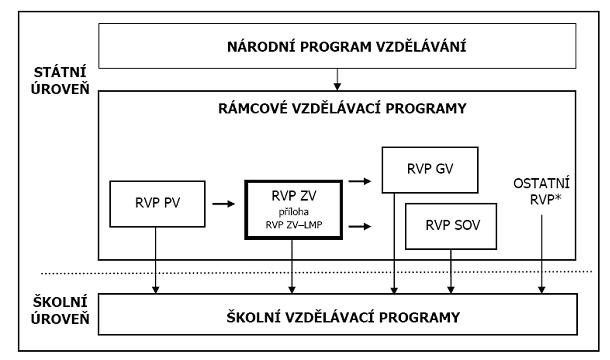
\includegraphics[width=0.8\linewidth]{fotky/rvpCR.jpg}
			\caption{\textbf{Ramcovy vzdelavaci program CR.}
				TODO 1-2 vety
			}
			\label{obr:rvpCR}
		\end{figure}


		Rámcový vzdělávací program pro předškolní vzdělávání je rozdělen do 12 kapitol.
		\begin{enumerate}[1.]
			\setlength\itemsep{-2mm}

			\item \textit{\uv{Vymezení Rámcového vzdělávacího programu pro předškolní vzdělávání v systému kurikulárních dokumentů
			\item Předškolní vzdělávání v systému vzdělávání a jeho organizace
			\item Pojetí a cíle předškolního vzdělávání
			\item Vzdělávací obsah RVP PV
			\item Vzdělávací oblasti
			\item Vzdělávací obsah ve školním vzdělávacím programu 
			\item Podmínky předškolního vzdělávání
			\item Vzdělávání dětí se speciálními vzdělávacími potřebami a dětí mimořádně nadaných
			\item Autoevaluace mateřské školy a hodnocení dětí
			\item Zásady pro zpracování školního vzdělávacího programu
			\item Kriteria souladu rámcového a školního vzdělávacího programu
			\item Povinnost předškolního pedagoga}} \citep[s.~2]{RVP}
		\end{enumerate}

		Pro tuto práci a možnosti komparace s francouzským kurikulem se budu podrobněji zabývat jen některými částmi RVP PV. A to kapitolou 5 Vzdělávací oblasti a kapitolou 3 Pojetí a cíle předškolního vzdělávání.

		Obsah RVP je udáván pouze obecně a rámcově, slouží jako prostředek k naplňování
		vzdělávacích záměrů a dosahování vzdělávacích cílů. Vzdělávací obsah RVP PV je rozdělen do pěti oblastí:

		\begin{enumerate}[1.]
			\setlength\itemsep{-2mm}
			\item Dítě a jeho tělo
			\item Dítě a jeho psychika
			\item Dítě a ten druhý
			\item Dítě a společnost
			\item Dítě a svět
		\end{enumerate}

		Každá oblast obsahuje 4 části. Těmi jsou dílčí vzdělávací cíle (co pedagog u dítěte podporuje), vzdělávací nabídka (co pedagog dítěti nabízí), očekávané výstupy (co dítě na konci předškolního období zpravidla dokáže) a rizika (co ohrožuje úspěch vzdělávacích záměrů pedagoga).

		Mají-li se srovnávat vzdělávací oblastí a jejich cíle u obou dokumentů, je potřeba v další kapitole uvést stručné obsahy vzdělávácích oblastí rámcového vzdělávacího programu pro předškolní vzdělávání České republiky. 

			\subsection{Dítě a jeho tělo}
				\textit{\uv{Záměrem vzdělávacího úsilí pedagoga v oblasti biologické je stimulovat a podporovat růst a neurosvalový vývoj dítěte, podporovat jeho fyzickou pohodu, zlepšovat jeho tělesnou zdatnost i pohybovou a zdravotní kulturu, podporovat rozvoj jeho pohybových a manipulačních dovedností, učit je sebeobslužným dovednostem a vést je k zdravým životním návykům a postojům.}} \citep[s.~16]{RVP}

				\paragraph{Dílčí vzdělávací cíle} 

				\begin{itemize}
				\setlength\itemsep{-2mm}
					\item[-]rozvoj jemné a hrubé motoriky
					\item[-]uvědomění si a ovládaní vlastního těla
					\item[-]rozvoj všech smyslů
					\item[-]rozvoj psych. a fyz. Zdatnosti
					\item[-]základní poznatky o zdraví a zdravém životním stylu
				\end{itemize}

					%Uvědomění si vlastního těla, zdokonalení jemné a hrubé motoriky, koordinace, ovládání pohybového aparátu, rozvoj všech smyslů, rozvoj fyzické i psychické zdatnosti, základní poznatky o těle, zdraví a zdravém životním stylu.

				\paragraph{Vzdělávací nabídka}

				\begin{itemize}
				\setlength\itemsep{-2mm}
					\item[-]lokomoční a manipulační hry
					\item[-]smyslové a psychomotorické hry
					\item[-]konstruktivní a grafické hry
					\item[-]hudební a hudebně pohybové hry
					\item[-]sebeosblužné činnosti
					\item[-]relaxační a odpočinkové činnosti
					\item[-]prevence úrazů, nemoci, závislostí
				\end{itemize}

					%Lokomoční pohybové hry, manipulační činnosti, smyslové a psychomotorické hry, konstruktivní a grafické hry, hudební a hudebně pohybové hry, sebeobslužné činnosti, relaxační a odpočinkové činnosti, příležitosti a činnosti směřující k prevenci úrazů, nemoci, nezdravých návyků a závislostí.

				\paragraph{Očekávané výstupy}

				\begin{itemize}
				\setlength\itemsep{-2mm}
					\item[-]správné držení těla
					\item[-]zvládnutí základních pohybových dovedností a prostorové orientace
					\item[-]koordinace lokomoce, koordinace ruky a oka a jemné motoriky
					\item[-]napodobování pohybů podle vzoru
					\item[-]ovládání dechového svalstva
					\item[-]vnímat a rozlišovat všemi smysly
					\item[-]zvládnutá sebeobsluha a hygienické návyky
					\item[-]pojmenovat části těla a jejich funkce
					\item[-]povědomí o ochraně osobního zdraví a kde hledat pomockonstruktivní
				\end{itemize}

					%Správné držení těla, zvládnutí základních pohybových dovedností a prostorové orientace, koordinace lokomoce a sladění pohybu s hudbou, napodobit jednoduchý pohyb podle vzoru, ovládat dechové svalstvo, vnímat a rozlišovat pomocí všech smyslů, zvládat koordinaci ruky a oka a jemnou motoriku, zvládnout sebeosluhu a hygienické návyky, zvládat pracovní úkony, pojmenovat části těla a znát jejich funkce, rozlišovat, co prospívá zdraví, mít povědomí o péči o čistotu, o způsobech ochrany osobního zdraví a kde hledat pomoc, zacházet s předměty denní potřeby.

			\subsection{Dítě a jeho psychika}
				\textit{\uv{Záměrem vzdělávacího úsilí pedagoga v oblasti psychologické je podporovat duševní pohodu, psychickou zdatnost a odZolnost dítěte, rozvoj jeho intelektu, řeči a jazyka, poznávacích procesů a funkcí, jeho citů i vůle, stejně tak i jeho sebepojetí a sebenahlížení, jeho kreativity a sebevyjádření, stimulovat jeho osvojování a rozvoj jeho vzdělávacích dovedností a povzbuzovat je v dalším rozvoji a učení.
				Tato oblast zahrnuje tři „podoblasti“: Jazyk a řeč‘; Poznávací schopnosti a funkce, představivost a fantazie, myšlenkové operace; Sebepojetí, city a vůle.}} \citep[s.~18]{RVP}
				\paragraph{I Jazyk a řeč}
				 
					\subparagraph{Dílčí vzdělávací cíle}

					\begin{itemize}
					\setlength\itemsep{-2mm}
						\item[-]rozvoj řečových schopností a jazykových dovedností  (receptivních i produktivních)
						\item[-]rozvoj řečových schopností a jazykových dovedností (receptivních a produktivních)
						\item[-]osvojení si dovedností předcházejících čtení a psaní
					\end{itemize}

						%Rozvoj řečových schopností a jazykových dovedností receptivních a produktivních, rozvoj komunikativních dovedností, osvojení si dovedností předcházejících čtení i psaní
					
					\subparagraph{Vzdělávací nabídka}

					\begin{itemize}
					\setlength\itemsep{-2mm}
						\item[-]artikulační, řečové, sluchové a rytmické hry
						\item[-]individuální a skupinová  konverzace
						\item[-]vyprávění, komentování zážitků, vyřizování vzkazů
						\item[-]poslech pohádek, filmové a divadelní příběhy
						\item[-]vyprávění, přednes, recitace,zpěv
						\item[-]grafické napodobování symbolů
						\item[-]poznávání a rozlišování zvuku a gest
						\item[-]seznámení se se sdělovacími prostředky
					\end{itemize}

						%Artikulační, řečové, sluchové a rytmické hry, individuální a skupinová konverzace, vyprávění, komentování zážitků, vyřizování vzkazů, poslech pohádek, sledování filmových a divadelních příběhů, vyprávění, přednes, recitace, zpěv, grafické napodobování symbolů, poznávání a rozlišování zvuků a gest, seznámení se se sdělovacími prostředky
					
					\subparagraph{Očekávané výstupy}

					\begin{itemize}
					\setlength\itemsep{-2mm}
						\item[-]správně vyslovovat, ovládat dech, tempo a intonaci řeči
						\item[-]vyjadřovat myšlenky, nápady, pocity
						\item[-]vést rozhovor, domluvit se slovy i gesty
						\item[-]porozumět slyšenému, formulovat otázky, odpovídat, slovně reagovat
						\item[-]umět krátké texty zpaměti, sledovat a vyprávět příběh, popsat situaci, chápat slovní humor
						\item[-]sluchově rozlišovat začáteční a koncové slabiky a hlásky ve slovech, utvořit jednoduchý rým
						\item[-]poznat některá písmena, číslice, své jméno
						\item[-]zájem o knížky, hudbu, film
					\end{itemize}

						%Správně vyslovovat, ovládat dech, tempo a intonaci řeči, vyjadřovat myšlenky, nápady, pocity, vést rozhovor, domluvit se slovy i gesty, porozumět slyšenému, formulovat otázky, odpovídat, slovně reagovat, naučit se krátké texty zpaměti, sledovat a vyprávět příběh, popsat situaci, chápat slovní humor, sluchově rozlišovat začáteční a koncové slabiky a hlásky ve slovech, utvořit jednoduchý rým, rozlišovat obrazné symboly, poznat některá písmena, číslice, své jméno, zájem o knížky, hudbu, film.
					
				
				\paragraph{II Poznávací schopnosti a funkce, představivost a fantazie, myšlenkové operace}
				\textcolor{white}{ } 

					\subparagraph{Dílčí vzdělávací cíle}

					\begin{itemize}
					\setlength\itemsep{-2mm}
						\item[-]rozvoj smyslového vnímání
						\item[-]rozvoj smyslového vnímání, paměti, pozornosti, představivosti a fantazie
						\item[-]rozvoj tvořivosti
						\item[-]posilování poznávacích citů
						\item[-]rozvoj zájmu o učení
						\item[-]osvojení si elementárních poznatků o znakových systémech
						\item[-]základ práce s informace
					\end{itemize}

						%Rozvoj smyslového vnímání, přechod k pojmovému myšlení, rozvoj paměti, pozornosti, představivosti a fantazie, rozvoj tvořivosti, posilování poznávacích citů (zvídavost, zájem…), podpora a rozvoj zájmu o učení, osvojení si elementárních poznatků o znakových systémech, základ práce s informacemi.
					
					\subparagraph{Vzdělávací nabídka}

					\begin{itemize}
					\setlength\itemsep{-2mm}
						\item[-]pozorování přírodních, kulturních a technických objektů a jevů
						\item[-]pojmenování jejich vlastností a charakteristických znaků
						\item[-]motivovaná manipulace s předměty
						\item[-]konkrétní manipulace s materiálem
						\item[-]smyslové hry
						\item[-]hry na rozvoj postřehu, vnímání, zrakové a sluchové paměti, pozornosti a různých druhů paměti
						\item[-]námětové hry, hry podporující tvořivost, představivost a fantazii
						\item[-]řešení myšlenkových i praktických problémů a hledaní řešení
						\item[-]činnosti k seznámení s matematickými pojmy a jejich symbolikou
						\item[-]činnosti zasvěcující do časových pojmů
					\end{itemize}

						%Pozorování přírodních, kulturních i technických objektů a jevů, pojmenovávání jejich vlastností a charakteristických znaků, motivovaná manipulace s předměty, konkrétní operace s materiálem, smyslové hry, hry na rozvoj postřehu a vnímání, zrakové a sluchové paměti, pozornosti a různých forem paměti, námětové hry, hry podporující tvořivost, představivost a fantazii, řešení myšlenkových i praktických problémů a hledání variant řešení, činnosti k seznámení se s matematickými pojmy a jejich symbolikou, činnosti zasvěcující dítě do časových pojmů.
					
					
					\subparagraph{Očekávané výstupy}

					\begin{itemize}
					\setlength\itemsep{-2mm}
						\item[-]vědomě využívat všech smyslů
						\item[-]záměrně pozorovat, všímat si, soustředit se a udržet pozornost
						\item[-]poznat a pojmenovat většinu toho, co ho obklopuje
						\item[-]přemýšlet a vést jednoduché úvahy
						\item[-]naučit se nazpaměť krátké texty
						\item[-]postupovat a učit se podle instrukcí, využívat zkušenost k učení
						\item[-]chápat základní číselné a matematické pojmy, souvislosti a prakticky je používat
						\item[-]chápat prostorové pojmy, elementární časové pojmy
						\item[-]řešit problémy, myslet kreativně, nalézat nová řešení
						\item[-]vyjadřovat představivost v tvořivých činnosti
					\end{itemize}

						%Vědomě využívat všech smyslů, záměrně pozorovat, všímat si, soustředit se a udržet pozornost, poznat a pojmenovat většinu toho, čím je obklopeno, přemýšlet a vést jednoduché úvahy, využívat zkušeností k učení, postupovat a učit se podle instrukcí, chápat základní číselné a matematické pojmy, souvislosti a prakticky je využívat, chápat prostorové pojmy, elementární časové pojmy, naučit se nazpaměť krátké texty, řešit problémy, myslet kreativně, nalézat nová řešení, vyjadřovat svou představivost v tvořivých činnostech.
					
				
				\paragraph{III Sebepojetí, city, vůle}
				
					\subparagraph{Dílčí vzdělávací cíle}

					\begin{itemize}
					\setlength\itemsep{-2mm}
						\item[-]poznávání sebe sama, rozvoj pozitivních citů k sobě
						\item[-]získání relativní citové samostatnosti
						\item[-]rozvoj schopnosti sebeovládání
						\item[-]vytváření osobních vazeb
						\item[-]rozvoj schopností vyjádřit prožitky a dojmy
						\item[-]rozvoj mravního i estetického vnímání
						\item[-]získání schopnosti záměrně řídit svoje chování a ovlivňovat vlastní situaci
					\end{itemize}

						%Poznávání sebe sama, rozvoj pozitivních citů k sobě, získání relativní citové samostatnosti, rozvoj schopnosti sebeovládání, vytváření citových vazeb, rozvoj schopností vyjádřit prožitky a dojmy, rozvoj mravního i estetického vnímání, získání schopnosti záměrně řídit svoje chování a ovlivňovat vlastní situaci.

					\subparagraph{Vzdělávací nabídka}
					
					\begin{itemize}
					\setlength\itemsep{-2mm}
						\item[-]spontánní hra
						\item[-]činnosti vyvolávající spokojenost, veselí, pohodu
						\item[-]úkoly, v nichž může být dítě úspěšné
						\item[-]činnosti vyžadující samostatné vystupování, obhajování vlastních názorů, rozhodování, sebeohodnocení
						\item[-]hry pro rozvoj vůle a sebeovládání
						\item[-]cvičení organizačních dovedností
						\item[-]estetické a tvůrčí aktivity, cvičení v projevování citů, v sebekontrole a sebeovládání
						\item[-]výlety do okolí
						\item[-]činnosti k poznávání různých lidských vlastností
						\item[-]dramatické činnosti, mimické vyjadřování
						\item[-]činnosti vedoucí k vyjádření sebe sama a k odlišení od ostatních
					\end{itemize}

						%Spontánní hra, činnosti vyvolávající spokojenost, veselí, pohodu, úkoly, v nichž může být dítě úspěšné, činnosti vyžadující samostatné vystupování, obhajování vlastních názorů, rozhodování, sebehodnocení, hry pro rozvoj vůle a sebeovládání, cvičení organizačních dovedností, estetické a tvůrčí aktivity, cvičení v projevování citů, v sebekontrole a v sebeovládání, hry na téma rodiny apod., výlety do okolí, činnosti k poznávání různých lidských vlastností, dramatické činnosti, mimické vyjadřování, činnosti vedoucí k identifikaci sebe sama a k odlišení od ostatních.
					
					\subparagraph{Očekávané výstupy}

					\begin{itemize}
					\setlength\itemsep{-2mm}
						\item[-]odloučit se na určitou dobu od rodičů, uvědomovat si svou samostatnost
						\item[-]zaujímat vlastní názory, rozhodovat o svých činnostech
						\item[-]vyjádřit souhlas i nesouhlas, uvědomovat si své možnosti i limity
						\item[-]přijímat pozitivní ocenění i případný neúspěch a vyrovnat se s ním
						\item[-]vyvinout volní úsilí, soustředit se na činnost a dokončit ji
						\item[-]zorganizovat hru a respektovat pravidla
						\item[-]rozlišovat citové projevy v různých prostředích, prožívat a projevovat, co cítí
						\item[-]snažit se ovládat afektivní chování
						\item[-]být citlivý k živým bytostem, přírodě i věcem
						\item[-]těšit se z příjemných zážitků
						\item[-]zachytit a vyjádřit své pocity
					\end{itemize}

						%Odloučit se na určitou dobu od rodičů a blízkých, uvědomovat si svou samostatnost, zaujímat vlastní názory, rozhodovat o svých činnostech, vyjádřit souhlas i nesouhlas, uvědomovat si své možnosti a limity, přijímat pozitivní ocenění i případný neúspěch a vyrovnat se s tím, prožívat radost ze zvládnutého, vyvinout volní úsilí, soustředit se na činnost a dokončit ji, respektovat pravidla, zorganizovat hru, rozlišovat citové projevy v důvěrném i cizím prostředí, prožívat a projevovat, co cítí, snažit se ovládat afektivní chování, být citlivý k živým bytostem, přírodě i věcem, těšit se z příjemných zážitků, zachytit a vyjádřit své pocity.
					

			\subsection{Dítě a ten druhý}
				\textit{\uv{Záměrem vzdělávacího úsilí pedagoga v interpersonální oblasti je podporovat utváření vztahů dítěte k jinému dítěti či dospělému, posilovat, kultivovat a obohacovat jejich vzájemnou komunikaci a zajišťovat pohodu těchto vztahů.}} \citep[s.~24]{RVP}

					\paragraph{Dílčí vzdělávací cíle}

					\begin{itemize}
					\setlength\itemsep{-2mm}
						\item[-]seznamování se s pravidly chování k druhému
						\item[-]osvojení si schopností a dovedností pro navazování a rozvíjení vztahů
						\item[-]posilován prosociálního chování
						\item[-]vytváření prosociálních postojů
						\item[-]rozvoj komunikativních a kooperativních dovedností
						\item[-]ochrana osobního soukromí
					\end{itemize}
						%Seznamování se s pravidly chování k druhému, osvojení si schopností a dovedností pro navazování a rozvíjení vztahů, posilování prosociálního chování, vytváření prosociálních postojů, rozvoj komunikativních a kooperativních dovedností, ochrana osobního soukromí.
					
					\paragraph{Vzdělávací nabídka}

					\begin{itemize}
					\setlength\itemsep{-2mm}
						\item[-]běžné komunikační aktivity dítěte s druhými
						\item[-]sociální hry, hraní rolí, dramatické činnosti
						\item[-]hudební a hudebně pohybové hry
						\item[-]aktivity podporující uvědomování si vztahů mezi lidmi
						\item[-]činnosti na porozumění pravidlům vzájemného soužití
						\item[-]hry vedoucí k ohleduplnosti k druhému, ochotě rozdělit se, pomoci si, vyřešit spor
						\item[-]činnosti na poznávání sociálního prostředí (rodina, MŠ)
						\item[-]hry, kdy se dítě učí chránit soukromí a bezpečí své i druhých
						\item[-]četba, vyprávění a poslech příběhu s etickým obsahem a ponaučením
					\end{itemize}

						%Běžné komunikační aktivity dítěte s druhými, sociální hry, hraní rolí, dramatické činnosti, hudební a hudebně pohybové hry, společenské hry a aktivity, kooperativní činnosti, společná setkávání a naslouchání ostatním, aktivity podporující uvědomování si vztahů mezi lidmi, činnosti na porozumění pravidlům vzájemného soužití, hry vedoucí k ohleduplnosti k druhému, ochotě rozdělit se, pomoci si, vyřešit spor, činnosti na poznávání sociálního prostředí-rodina, mateřská škola; hry a situace, kdy se dítě učí chránit soukromí a bezpečí své i druhých, četba, vyprávění a poslech příběhů s etickým obsahem a ponaučením.
					
					\paragraph{Očekávané výstupy}

					\begin{itemize}
					\setlength\itemsep{-2mm}
						\item[-]navazovat kontakty s dospělým, kterému je svěřeno do péče
						\item[-]komunikovat s ním, respektovat ho, porozumět projevům emoci a nálad
						\item[-]přirozeně komunikovat s druhým dítětem, navazovat přátelství,
						\item[-]uvědomovat si svá práva a respektovat práva ostatních
						\item[-]uplatňovat své individuální potřeby a přání s ohledem na druhé
						\item[-]dodržovat pravidla vzájemného soužití v různých prostředích i pravidla her
						\item[-]respektovat potřeby jiného dítěte, dělit se s ním o věci
						\item[-]vycházet vstříc ostatním a pomáhat jim
						\item[-]bránit se projevům násilí
						\item[-]chovat se obezřetně při setkáních s neznámými dětmi a dospělými
					\end{itemize}

						%Navazovat kontakty s dospělým, kterému je svěřeno do péče, komunikovat s ním, respektovat ho, porozumět projevům emocí a nálad, přirozeně komunikovat s druhým dítětem, navazovat přátelství, uvědomovat si svá práva, respektovat práva ostatních, spolupracovat s ostatními, uplatňovat své individuální potřeby a přání s ohledem na druhé, dodržovat pravidla vzájemného soužití v různých prostředích i pravidla her, respektovat potřeby jiného dítěte, dělit se s ním o věci, vycházet vstříc ostatním a pomáhat jim, bránit se projevům násilí, chovat se obezřetně při setkání s neznámými dětmi a dospělými.
					

			\subsection{Dítě a společnost}
				\textit{\uv{Záměrem vzdělávacího úsilí pedagoga v oblasti sociálně-kulturní je uvést dítě do společenství ostatních lidí a do pravidel soužití s ostatními, uvést je do světa materiálních i duchovních hodnot, do světa kultury a umění, pomoci dítěti osvojit si potřebné dovednosti, návyky i postoje a umožnit mu aktivně se podílet na utváření společenské pohody ve svém sociálním prostředí.}} \citep[s.~26]{RVP}

					\paragraph{Dílčí vzdělávací cíle}

					\begin{itemize}
					\setlength\itemsep{-2mm}
						\item[-]poznávání pravidel společenského soužití a jejich spoluvytváření
						\item[-]porozumění základním projevům neverbální komunikace v tomto prostředí
						\item[-]rozvoj schopnosti žít ve společenství ostatních lidí a přijímat základní hodnoty v tomto společenství uznávané
						\item[-]rozvoj základních kulturně společenských postojů
						\item[-]rozvoj schopnost projevovat se autenticky a autonomně
						\item[-]vytvoření povědomí o morálních hodnotách
						\item[-]seznamování se světem lidí, kultury a umění
						\item[-]vytváření povědomí o jiných kulturách, rozvoj společenského i estetického vkusu
					\end{itemize}

						%Poznávání pravidel společenského soužití a jejich spoluvytváření, porozumění základním projevům neverbální komunikace v tomto prostředí, rozvoj schopnosti žít ve společenství ostatních lidí a přijímat základní hodnoty v tomto společenství uznávané, rozvoj základních kulturně společenských postojů, rozvoj schopnosti projevovat se autenticky a autonomně, vytvoření povědomí o morálních hodnotách, seznamování se světem lidí, kultury a umění, vytváření povědomí o jiných kulturách, rozvoj společenského i estetického vkusu.

					\paragraph{Vzdělávací nabídka}

					\begin{itemize}
					\setlength\itemsep{-2mm}
						\item[-]setkávání s pozitivními vzory vztahů a chování
						\item[-]aktivity pro adaptaci dítěte v MŠ
						\item[-]společenské hry a skupinové aktivity umožňující dětem se spolupodílet na jejich průběhu
						\item[-]přípravy a realizace společenských zábav a slavností
						\item[-]tvůrčí a receptivní činnosti slovesné, literární, dramatické, výtvarné apod.
						\item[-]návštěvy kulturních a uměleckých míst
						\item[-]hry na poznávání různých společenských rolí
						\item[-]aktivity přibližující pravidla vzájemného styku a mravní hodnoty
						\item[-]hry a praktické činnosti uvádějící dítě do světa lidí, jejich občanského života a práce
						\item[-]aktivity přibližující svět kultury a umění a umožňující poznat rozmanitost kultur
					\end{itemize}

						%Setkávání s pozitivními vzory vztahů a chování, aktivity pro adaptaci dítěte v MŠ, společenské hry a skupinové aktivity umožňující dětem se spolupodílet na jejich průběhu, přípravy a realizace společenských zábav a slavností, tvůrčí a receptivní činnosti slovesné, literární, dramatické, výtvarné apod., setkávání se s uměním mimo MŠ, návštěvy kulturních a uměleckých míst, hry na poznávání různých společenských rolí, aktivity přibližující pravidla vzájemného styku a mravní hodnoty, hry a praktické činnosti uvádějící dítě do světa lidí, jejich občanského života a práce, aktivity přibližující svět kultury a umění a umožňující poznat rozmanitost kultur.
					
					\paragraph{Očekávané výstupy}

					\begin{itemize}
					\setlength\itemsep{-2mm}
						\item[-]uplatňovat návyky společenského chování ve styku s dospělými i dětmi
						\item[-]pochopit, že každý má ve společenství svou roli a podle ní se chovat
						\item[-]chovat se dle vlastních pohnutek, ale s ohledem na druhé
						\item[-]začlenit se do třídy a respektovat rozdílné vlastnosti vrstevníků
						\item[-]porozumět běžným neverbálním projevům citových prožitků a nálad druhých
						\item[-]adaptovat se ve škole a zvládat požadavky prostředí
						\item[-]vyjednávat s ostatními a domluvit se na společném řešení
						\item[-]utvořit si základní dětskou představu o pravidlech chování a společenských normách a chovat se dle toho
						\item[-]jednat spravedlivě, hrát fair, dodržovat pravidla her, 
						\item[-]odmítat společensky nežádoucí chování a chránit se pře ním
						\item[-]vnímat umělecké podněty a hodnotit svoje zážitky
						\item[-]vyjadřovat se pomoci výtvarných technik a prostřednictvím hudeních a hudebně pohybových činností
					\end{itemize}

						%Uplatňovat návyky společenského chování ve styku s dospělými i dětmi, pochopit, že každý má ve společenství svou roli a podle ní se chovat, chovat se dle vlastních pohnutek, ale s ohledem na druhé, začlenit se do třídy a respektovat rozdílné vlastnosti vrstevníků, porozumět běžným neverbálním projevům citových prožitků a nálad druhých, adaptovat se ve škole a zvládat požadavky prostředí, vyjednávat s ostatními a domluvit se na společném řešení, utvořit si základní dětskou představu Dítě a světo pravidlech chování a společenských normách a chovat se dle toho, chovat se zdvořile, s úctou a bez předsudků, dodržovat pravidla her, jednat spravedlivě, hrát fair, odmítat společensky nežádoucí chování a chránit se pře ním, vnímat umělecké podněty a hodnotit svoje zážitky, vyjadřovat skutečnost pomocí různých výtvarných technik, vyjadřovat se prostřednictvím hudebních a hudebně pohybových činností.
					

			\subsection{Dítě a svět}
				\textit{\uv{Záměrem vzdělávacího úsilí pedagoga v environmentální oblasti je založit u dítěte elementární povědomí o okolním světě a jeho dění, o vlivu člověka na životní prostředí – počínaje nejbližším okolím a konče globálními problémy celosvětového dosahu – a vytvořit elementární základy pro otevřený a odpovědný postoj dítěte (člověka) k životnímu prostředí.}} \citep[s.~29]{RVP}

				\paragraph{Dílčí vzdělávací cíle}

				\begin{itemize}
				\setlength\itemsep{-2mm}
					\item[-]seznamování sea vytváření pozitivního vztahu k místu a prostředí, ve kterém dítě žije
					\item[-]poznávání jiných kultur
					\item[-]vytváření povědomí o širším přírodním, kulturním i technickém prostředí
					\item[-]pochopení, že lidská činnost může prostředí chrání, ale i ničit
					\item[-]osvojení si poznatků péče o okolí a spoluvytváření zdravého prostředí
					\item[-]rozvoj úcty k životu ve všech jeho formách
					\item[-]rozvoj schopnosti přizpůsobovat se podmínkám prostředí
					\item[-]vytvoření povědomí o vlastní sounáležitosti se světem
				\end{itemize}

					%Seznamování se a vytváření pozitivního vztahu k místu a prostředí, ve kterém dítě žije, poznávání jiných kultur, vytváření povědomí o širším přírodním, kulturním i technickém prostředí, pochopení, že lidská činnost může prostředí chránit, ale i ničit, osvojení si poznatků péče o okolí a spoluvytváření zdravého prostředí, rozvoj úcty k životu ve všech jeho formách, rozvoj schopnosti přizpůsobovat se podmínkám prostředí, vytvoření povědomí o vlastní sounáležitosti se světem.
				
				\paragraph{Vzdělávací nabídka}

				\begin{itemize}
				\setlength\itemsep{-2mm}
					\item[-]přirozené pozorování prostředí a života v něm
					\item[-]aktivity zaměřené na praktickou orientaci v obci
					\item[-]poučení o možných nebezpečných situacích a způsobech, jak se chránit
					\item[-]aktivity na téma dopravy, cvičení bezpečného chování v dopravních situacích
					\item[-]poznávání přírodního okolí, sledování rozmanitostí a změn v přírodě
					\item[-]využívání encyklopedií a obrazového materiálu
					\item[-]kognitivní činnosti, praktické činnosti k seznámení s materiály
					\item[-]pozorování životních podmínek a životního prostředí a okolní krajinu
				\end{itemize}

					%Přirozené pozorování prostředí a života v něm, aktivity zaměřené na praktickou orientaci v obci, účast na zajímavých akcích v obci, poučení o možných nebezpečných situacích a způsobech, jak se chránit, aktivity na téma dopravy, cvičení bezpečného chování v dopravních situacích, poznávání přírodního okolí, sledování rozmanitostí a změn v přírodě, využívání encyklopedií a obrazového materiálu, kognitivní činnosti, praktické činnosti k seznámení s materiály, pozorování životních podmínek a životního prostředí, ekohry, smysluplné činnosti přispívající k péči o životní prostředí a okolní krajinu.
				
				\paragraph{Očekávané výstupy}

				\begin{itemize}
				\setlength\itemsep{-2mm}
					\item[-]bezpečně se orientovat ve známém prostředí
					\item[-]zvládat běžné činnosti a požadavky na dítě kladené
					\item[-]chovat se přiměřeně a bezpečně doma i na veřejnosti
					\item[-]uvědomovat si nebezpečí a jak se může chránit
					\item[-]osvojit si elementární poznatky o okolním prostředí
					\item[-]vnímat, že svět má svůj řád, že je rozmanitý a pestrý
					\item[-]všímat si změn v okolí a porozumět, že změny jsou přirozené a samozřejmé
					\item[-]mít povědomí o významu životního prostředí
					\item[-]pomáhat pečovat o okolní prostředí a rozlišovat aktivity, které mohou zdraví okolního prostředí podporovat či poškozovat
				\end{itemize}

					%Bezpečně se orientovat ve známém prostředí, zvládat běžné činnosti a požadavky na dítě kladené, chovat se přiměřeně a bezpečně doma i na veřejnosti, uvědomovat si nebezpečí a jak se může chránit, osvojit si elementární poznatky o okolním prostředí, vnímat, že svět má svůj řád, že je rozmanitý a pestrý, všímat si změn v okolí a porozumět, že změny jsou přirozené a samozřejmé, mít povědomí o významu životního prostředí, pomáhat pečovat o okolní životní prostředí a rozlišovat aktivity, které mohou zdraví okolního prostředí podporovat a které poškozovat.

 			\subsection{Shrnutí pojetí a cílů předškolního vzdělávání a role pedagoga}

				Pojetím a cíli předškolní vzdělávání se v českém dokumentu věnuje samostatná kapitola \uv{Pojetí a cíle předškolního vzdělávání}. Níže je uvedeno shrnutí důležitých témat včetně vymezení role pedagoga a doporučení pro jeho práci, volbu vhodných metod vzdělávání a postupů. Výstupy vzdělávácích cílů předškolního zvdělávání jsou formulovány jako klíčové kompetence			

				Mezi hlavní principy RVP PV patří akceptování přirozených vývojových specifik dětí předškolního věku, vzdělávání dítěte v rozsahu jeho individuálních možností a potřeb, vytváření základů a osvojení si klíčových kompetencí (viz níže) dosažitelných v etapě předškolního vzdělávání a získávání předpokladů pro celoživotní vzdělávání.
				Předškolní vzdělávání má dítěti usnadňovat jeho další životní i vzdělávací cestu, rozvíjet jeho osobnost, tělesný rozvoj a zdraví, osobní spokojenost a pohodu a napomáhat mu v chápání okolního světa a motivovat jej k dalšímu poznávání, stejně tak jako učit dítě žít ve společnosti ostatních a přibližovat mu normy a hodnoty uznávané touto společností.
				Vhodnými metodami vzdělávání je dle RVP PV prožitkové a kooperativní učení hrou. Jde o činnosti, které jsou založeny na přímých zážitcích dítěte, které podporují dětskou zvídavost a potřebu objevovat, podněcují jeho radost z učení a jeho zájem poznávat nové věci a získávat nové zkušenosti.
				RVP řadí situační učení a spontánní sociální učení mezi významné procesy učení, které by měly být dostatečně zastoupeny. Aktivity by se měly střídat spontánní i řízené a měly by být vzájemně provázané a vyvážené. Pedagog by měl být průvodcem dítěte, probouzet v něm aktivní zájem a chuť dívat se kolem sebe, naslouchat a objevovat. Není zde ten, co „úkoluje“ a kontroluje. Didaktický styl by měl být založen na principu vzdělávací nabídky, na individuální volbě dítěte a jeho aktivní účasti.
				

				Důležitou složkou RVP PV jsou výstupy vzdělávacích cílů. Těmi jsou klíčové kompetence, neboli kompetence, které by děti měly ovládat na konci mateřské školy a před vstupem do školy základní. Je zde uváděno 5 kompetencí. Ke každé z nich uvedu opět stručný výtah:

				\paragraph{Kompetence k učení}
				\begin{itemize}
				\setlength\itemsep{-2mm}
				\item[-] elementární poznatky o světě lidí, kultuře, přírodě a technice, která dítě obklopuje
				\item[-] orientace se v řádu dění
				\item[-] klást otázky a hledat na ně odpovědi
				\item[-] aktivně si všímat a chtít porozumět jevům, které kolem sebe vidí
				\item[-] soustředěně pozorovat, objevovat, experimentovat a získanou zkušenost dále uplatňovat
				\item[-] učení probíhá spontánně, vědomě, s chutí
				\item[-] schopnost soustředit se na činnost a dokončit práci
				\item[-] postupovat podle instrukcí, odhadovat své síly 
				\end{itemize}
				

				\paragraph{Kompetence k řešení problémů}
				\begin{itemize}
				\setlength\itemsep{-2mm}
				\item[-] všímat si dění i problémů okolo sebe
				\item[-] známé situace řešit samostatně, náročnější s oporou a pomocí dospělého
				\item[-] řešit problémy  na základě bezprostřední zkušenosti, cestou pokusu a omylu experimentovat, vymýšlet nová řešení, hledat varianty
				\item[-] využívat dosavadních zkušeností, fantazii a představivost 
				\item[-] užívat logických, matematických a empirických postupů 
				\item[-] dovednost volit mezi řešením vedoucím k cíli a řešením nefunkčním
				\item[-] nebát se chybovat
				\end{itemize}
				

				\paragraph{Kompetence komunikativní}
				\begin{itemize}
				\setlength\itemsep{-2mm}
				\item[-] v běžných situacích komunikovat bez zábran a ostychu s dětmi i s dospělými
				\item[-] ovládat řeč, samostatně vyjadřovat své myšlenky ve vhodně formulovaných větách
				\item[-] dokázat sdělit své prožitky a pocity a to všemi prostředky (i výtvarnými, hudebními, dramatickými). 
				\item[-] ovládat dovednosti předcházející čtení a psaní 
				\item[-] mít povědomí o existenci jiných jazyků
				\item[-] průběžně rozšiřovat slovní zásobu aaktivně ji používat
				\item[-] využívat informativní a komunikační prostředky (telefon, knihy, počítač…)
				\end{itemize}

				\paragraph{Kompetence sociální a personální}
				\begin{itemize}
				\setlength\itemsep{-2mm}
				\item[-] samostatně se rozhodovat o svých činnostech
				\item[-] umět si vytvořit a vyjádřit svůj názor
				\item[-] uvědomovat si, že odpovídá za své jednání, projevovat citlivost a ohleduplnost k druhým, vnímat nespravedlnost a ubližování
				\item[-] domlouvat se a spolupracovat při společenských činnostech
				\item[-] uplatňovat pravidla společenského styku a dodržovat dohodnutá pravidla 
				\item[-] respektovat druhé a uzavírat kompromisy. 
				\item[-] umět být tolerantní k odlišnostem druhých lidí.
				\item[-] dokázat se bránit násilí a ponižování
				\end{itemize}

				\paragraph{Kompetence činnostní a občanské}
				\begin{itemize}
				\setlength\itemsep{-2mm}
				\item[-] dokázat rozpoznat svoje silné a slabé stránky
				\item[-] učit se plánovat, organizovat a vyhodnocovat svoje činnosti a hry
				\item[-] odhadovat rizika svých nápadů a dokázat se přizpůsobovat okolnostem
				\item[-] chápat, že se může svobodně rozhodovat, ale i že nese odpovědnost za svá rozhodnutí
				\item[-] zajímat se o druhé a co se děje kolem
				\item[-] mít smysl pro povinnost ve hře, práci i učení
				\item[-] Uvědomuje si svá práva i práva druhých
				\item[-] uvědomovat si, že svým chováním ovlivňuje prostředí, ve kterém žije, a dbát na osobní zdraví a bezpečí své i druhých
				\end{itemize}



\begin{landscape}
\begin{table}[t]
\center
\begin{tabular}{|c|c|c|l|}
\rowcolor{grey}
\hline			
				& \textbf{Francie}			& \textbf{Česká republika}	& \textbf{Rozdíly} 	\\
\hline
\hline
\rowcolor{grey!10}
Dokument	& státní, veřejně dostupný		& státní, veřejně dostupný 	& 			\\	\rowcolor{grey!50}
Rozsah		& 12 kapitol	 				& 11 kapitol	&						\\  \rowcolor{grey!10}
Předškolnímu vzdělání	& celý dokument			& 2 kapitoly	& FR: vzdělávání na půdě MŠ  zasahuje 	\\ \rowcolor{grey!10}
se věnuje				&						&				& do dvou vzdělávacích cyklů, proto  	\\ \rowcolor{grey!10}
				&								& 				& je prezentován v jednom dokumentu  	\\ \rowcolor{grey!10}
				&								&				& společně s ostatními cykly.    		\\ \rowcolor{grey!10}
				&								&				& ČR: preprimární vzdělávání odděleno 	\\ \rowcolor{grey!10}
				&								&				& od základního, věnuje se mu tedy  	\\ \rowcolor{grey!10}
				&								&				& samostatný dokument.					\\ 
\rowcolor{grey!50}
Kompetence		& na konci každé 				& hlavní výstupy  	&		\\	\rowcolor{grey!50}
				& vzdělávací oblasti 			& vzdělávacích cílů & 		\\
\rowcolor{grey!10}
Vzdělávací oblasti	& 6							& 5 					& FR: vzdělávací oblasti určují čeho 	\\	
\rowcolor{grey!10}
					& Osvojit si řeč			& Dítě a jeho tělo		& má dítě dosáhnout.					\\
\rowcolor{grey!10}
					& Objevovat písmo 			& Dítě a jeho psychika	& ČR: vzdělávací oblasti jsou sestave- \\
\rowcolor{grey!10}
					& Stát se žákem				& Dítě a ten druhý	 	& né z pozice dítěte k obsahu. 			\\
\rowcolor{grey!10}
					& Jednat a vyjadřovat se 	& Dítě a společnost 	& 	 									\\
\rowcolor{grey!10}
					& vlastním tělem			& Dítě a svět			& 	 									\\
\rowcolor{grey!10}
					& Objevovat svět			& 			 			& 	\\	
\rowcolor{grey!10}
					& Vnímat, cítit, 			& 						& 	\\
\rowcolor{grey!10}
					& představovat si, tvořit 	&						& 	\\		
\rowcolor{grey!50}
Dílčí vzdělávací cíle	& ANO					& ANO 					& 	\\	
\rowcolor{grey!10}
Vzdělávací nabídka	& Okrajově popsána	 		& Podrobně popsána	 	& Ve FR je dán větší prostor učitelům, 	\\
\rowcolor{grey!10}
					&							&						& jak budou práci koncipovat. 			\\
\rowcolor{grey!10}
					&							&						& V ČR je tento prostor užší, nabídka 	\\
\rowcolor{grey!10}
					&							&						& je přesněji určena. 					\\
\rowcolor{grey!50}
Očekávané výstupy	& Formulované jako 				& Detailně popsány pro 		& 		\\ 
\rowcolor{grey!50}
					& kompetence na konci kapitoly 	& každou vzdělávací oblast 	& 		\\
\rowcolor{grey!10}
Rizika	 			& NE						& ANO	 						& 		\\
\hline
\end{tabular}
\caption{ \textbf{Srovnání kurikul Francie a České republiky.}
	TODO: 1-2 vety o tom co tabulka shrnuje, aby sla pochopit bez cteni textu. Praesent neque justo, vehicula eget, interdum id, facilisis et, nibh. Phasellus at purus et libero lacinia dictum. Fusce aliquet.
}
\label{tab:srovnaniKurikul}
\end{table}
\end{landscape}

\section{Srovnání kurikul Francie a České republiky}

	Kurikulární dokumenty obou srovnávaných zemí, tedy Francie a České republiky, mají stejné legislativní zázemí. Jsou to státní dokumenty zakotvené ve školském zákoně a oba jsou volně dostupné široké veřejnosti, jak pedagogické tak nepedagogické. 

	Rozsah obou dokumentů je téměř shodný, ale český Rámcový vzdělávací plán je zaměřen pouze na předškolní vzdělávání a podrobně se věnuje všem oblastem, včetně začleňování dětí se speciálními potřebami, podmínkám předškolního vzdělávání, autoevaluaci mateřských škol i tvorbě školních vzdělávacích plánů. Jeho obsah je vyčerpávající a zahrnuje všechny okolnosti, v nichž se odehrává vývoj dítěte. Oproti tomu je francouzský dokument rozsahem kratší a věnuje se zvláště vzdělávacím oblastem a cílům vzdělávání. Poslední třída mateřské školy je zároveň první třídou druhého vzdělávacího cyklu. Jde o plynulý přechod na základní školu, tomu odpovídá i obsah vzdělávání, jak mateřské školy, tak prvních tříd školy základní. Cykly na sebe přirozeně navazují. Z tohoto důvodu je program mateřských škol prezentován ve stejném dokumentu jako program primárního vzdělávání a je mu věnována jeho poměrná část.

	Cíle v českém RVP PV jsou podrobně rozpracovány na záměry a výstupy na obecné a oblastní úrovni. Formulovanými výstupy vzdělávacích cílů je 5 klíčových kompetencí, které jsou detailně popsány a k jejichž naplňování by mělo směřovat veškeré vzdělávání. Ve francouzském Programu pro mateřské školy jsou kompetence zmíněné též, ale jsou uvedeny na konci každé vzdělávací oblasti.

	Formulačně jsou vzdělávací oblasti obou dokumentů odlišné, ale při detailnějším čtení je zřejmé, že přestože jsou vzdělávací oblasti zařazené do jiných skupin, obsahují oba dokumenty všechny oblasti, které je u dětí potřeba systematicky rozvíjet. Nejmarkantnějšími rozdíly jsou ve francouzském programu oblasti \textbf{Objevovat písmo} (Découvrir l´écrit) a \textbf{Stát se žákem} (Devenir élève).

	Již od 20. století je ve Francii kladen velký důraz na nácvik psaní. Na konci mateřské školy by děti měly ovládat velká tiskací písmena. Jak je v programu uvedeno, některým dětem se předkládá již písmo psací. Děti hodně kopírují slova z předloh, jako jsou dny v týdnu a názvy měsíců v roce a učí se svému podpisu. V České republice se jedná spíše o přípravu na psaní. Uvolňování svalů ruky, správné držení pera či tužky, nácvik grafomotoriky. Děti si uvědomují tvary, učí se volné ruce, ale neučí se psát a nekopírují. Písmena píší, jen když to vychází z jejich vlastního zájmu. 

	Název druhé zmíněné oblasti \textbf{Stát se žákem} evokuje přípravu na základní školu, a že se dítě po skončení mateřské školy stane \uv{žákem}. Její obsah je společný s českými oblastmi Dítě a ten druhý a Dítě a společnost, přestože z pouhého názvu kapitol to není na první pohled patrné. Shoda obou zemí je ve formálním obsahu, ovšem v pojetí hlavních vzdělávacích cílů se obě země diametrálně liší.

	Ve Francii si mateřská škola dává za úkol dostatečně dětem vštípit kompetence a znalosti, které povedou k úspěšnému zvládnutí základní školy. Formuje žáky a uvádí je do světa psaného jazyka a tím pádem i do světa čtení. Během pozorování byl ve Francii znatelný rozdíl v přístupu učitelů k dětem, kterému se krátce věnuji v závěru kapitoly~\ref{srovnani}. Učitel rozdával \uv{úkoly}, děti \uv{pracovaly} viz.~\ref{ateliery}. Autorka na základě kurikula a vzdělávacích cílů vyvozuje, že na dítě je ve Francii pohlíženo jako na \uv{žáka} a tak se k němu také přistupuje. 

	%Tomu odpovídá i tabulka, viz příloha., z které je patrné, že čas určený na různé aktivity, oběd, příchod a odchod velmi blízce kopíruje časový harmonogram výuky na základních školách. 
	%TODO odkaz na tabulku, takhle:

	Mezi cíle předškolního vzdělávání v České republice patří rozvoj osobnosti dítěte, jeho samostatnosti, rozvoj učení a poznávání a osvojení si hodnot naší společnosti. Vzdělávací oblasti jsou vzájemně provázány a respektují přirozenost dítěte a jeho postupné začleňování do životního a sociálního prostředí. 

	Autorka má dojem, že oproti Francii je v českém předškolním vzdělávání více respektováno a podporováno období dětství, s jeho vývojovými potřebami a specifiky. Z čehož usuzuje, že v České republice je na dítě pohlíženo ja na \uv{dítě}.

\chapter{REŽIM DNE}
\label{kap:rezim}
	Režimem dne je v tomto případě myšlený časový rozvrh aktivit během dne. Čili kdy a jaké činnosti se v průběhu dne konají. Spadá sem i příchod a odchod dětí z mateřské školy. Tato kapitola vychází z volného pozorování během povinných praxí v rámci studia. Věnuji se zde i zázemí tříd daných mateřských škol obou srovnávaných zemí, které je na první pohled odlišné a které mi přišlo též důležité, protože dává představu o tom, kde a za jakých podmínek se den v mateřské škole odehrává. 

	\section{Režim dne ve francouzské mateřské škole}

		Možnost věnovat se pozorování průběhu dne ve francouzské mateřské škole jsem měla v rámci povinné praxe během výměnného studijního programu Erasmus. Stáž se konala ve státní mateřské škole na předměstí Paříže, která spolupracuje s Academie Versaille pod Université de Cergy-Pontoise. Mateřskou školu jsem navštěvovala každý den po dobu dvou týdnů od 9h do 16h30, tedy po celou otevírací dobu. Mateřská škola byla otevřena každý pracovní den kromě středy. 

		\subsection{Zázemí mateřské školy}

			Mateřská škola je součástí velké budovy, kde se nachází i škola základní. Děti mají přístup na dvůr, který má na většině plochy betonový povrch a na části speciální měkký povrch, dvě prolézačky, pískoviště. Děti mají na dvoře k dispozici odstrkovadla, tříkolky a míče. 
			Mateřská škola se nachází v přízemí budovy a má 8 tříd, z čehož dvě jsou v prvním patře, v prostorách 	základní školy. Dále se zde nachází knihovna, tělocvična, dvě ložnice na spaní, sborovna a jídelna. 
			Kapacita mateřské školy v roce 2010 byla 250 dětí, maximální kapacita dětí ve třídě je 30 dětí. Tato kapacita byla ve většině tříd naplněna.

		\subsection{Třída a její vybavení}
		\label{sec:tridaVybaveni}
			Třída, ve které jsem absolvovala praxi, byla nevelká místnost, plně zaplněná nábytkem a pomůckami. Na zemi byla dlažba, jen na malé části před tabulí byl položen koberec. Místnost měla dvoje dveře. Jedny vedly ze školní chodby, druhé přímo na dvůr školy. Na jedné straně třídy dominovala na zdi pověšená tabule, na které byly přilepené různé cedulky s návody, jak se píší číslice 1-9, další číslice až do 30, cedulky se dny v týdnu, měsíci, datem a popisem ateliéru (Obr.~\ref{Obr1}). Před tabulí byly do kruhu postaveny 3 lavice na sezení. Po obou stranách tabule byly umístěny stolky s dětskými počítači (Obr.~\ref{Obr2}). Uprostřed třídy bylo postaveno 5 stolů, každý s 6 židličkami. Na protilehlé straně třídy se nacházel čtenářský koutek s křesílkem, umyvadla, police na výtvarný materiál, stůl pro paní učitelku, dětská kuchyňka s popisky věcí, které patří do kuchyně (Obr.~\ref{Obr3},~\ref{Obr4},~\ref{Obr5}). Na této straně byla na zdi pověšená písmena abecedy velikost A3 (Obr.~\ref{Obr6}). Čtenářský koutek i kuchyňka byly od třídy odděleny různými skříňkami a poličkami, které sloužily k uskladnění didaktických pomůcek a her či sešitů dětí (Obr.~\ref{Obr7}).


			Třída byla velmi dobře vybavena, co se týče materiálu i didaktických pomůcek. Do relativně malého prostoru se vešlo všechno potřebné. Nicméně pro volnou hru a volný pohyb dětí příliš místa nezbývalo. Na volnou hru se dal využít menší prostor s kobercem před tabulí a v dětské kuchyňce. Dále už zbývala jen volnější plocha přede dveřmi na dvůr a ulička napříč třídou. Tento prostor byl pro 29 dětí velmi malý. 
			Děti mají na výběr různé stolní hry, puzzle, knihy. Hraček se tu nacházelo minimum, pár plyšáků, nějaké autíčko. Pokud si děti donesly nějakou hračku z domova, musely ji na začátku hodiny odložit na poličku, kde na ně čekala až do odchodu ze třídy. 

		\subsection{Počet dětí a pedagogické zastoupení}

			Měla jsem možnost být ve třídě “Grand section“, kde jsou děti ve věku 5 let, poslední rok před nástupem na základní školu. Ve třídě bylo zapsáno 29 dětí, mateřskou školu jich v průměru navštěvovalo 25. Děti trávily v mateřské škole celý den. Na tuto třídu byla jedna paní učitelka a to od pondělí do pátku po celou otevírací dobu mateřské školy. S nikým se nestřídala. 

		\subsection{Pravidla chování}
		\label{pravidlaChovani}
			Při pohledu na třídu upoutá pozornost červený a zelený papír velikosti A3, na kterém byly přilepeny obrázky s pravidly, které by se měly ve třídě dodržovat. Na pravidla se vyučující odkazovala téměř pokaždé, když byla některá z nich porušena. Většinou dítě, které nějakým způsobem pravidla nedodrželo, bylo vyzváno, aby ukázalo, o které pravidlo jde a povědělo všem, jak by se mělo chovat. 

% TODO: do dvou sloupcu
+	Papír se vyhazuje do koše
	Hlásit se
	Uklízet po sobě materiál
	Řadit se do řady
	Být potichu
	Udržovat stoly čisté
Říkat „Dobrý den“, „Na shledanou“, „Děkuji“

- 	Neprat se
	Neběhat po třídě
	Nestrkat se
	Nekřičet
	Neničit materiál
	Neschovávat věci
	Neříkat sprostá slova
	Nekrást
	Neobtěžovat kamarády
(Obr.~\ref{Obr8})

		\subsection{Průběh dne a jeho specifika}

			Časový harmonogram visí v tištěné podobě na dveřích každé třídy a je závazný. Vyučující se snaží dané časy striktně dodržovat.

% TODO: do tabulky, aby to bylo hezky
8:50 – 9:10	Příchod dětí a jejich uvítání (volná hra, dokončování prací z minulého dne, úklid)
9:10 – 9:20			Rituály (pozdravení se, datum, počasí, představení ateliérů)
9:30 – 10:05			Ateliéry (grafomotorika/psaní, matematika, čtení)
10:05 – 10:15			Kruh (úklid, básničky/říkanky)
10:15 – 10:45			Přestávka
10:45 – 11:30			Lingvistické aktivity, společné čtení
11:30 – 11:50			Společný kruh (říkanky, matematické hry)
11:50 – 13:30			Oběd
13:30 – 13:55			Společný kruh (zpěv, hlasová cvičení, poslech)
13:55 – 14:30			Ateliéry (motorika, výtvarná výchova, objevování světa)
14:30 – 15:00			Tělocvična
15:00 – 15:30			Přestávka
15:30 – 16:10			Video nebo promítání diapozitivů
16:10 – 16:20			Úklid třídy, zhodnocení dne
16:20 – 16:30			Odchod dětí

			Zajímavostí francouzských mateřských škol je 4 denní týden. Děti navštěvují mateřskou školu jen v pondělí, úterý, čtvrtek a pátek. Ve středu jsou děti doma nebo mají volnočasové aktivity a sporty. Některé školy tyto aktivity nabízejí, jiné ne. 

		\subsection{Příchod dětí do třídy}
		\label{prichod}
			Brána školy je otevřena od 8h50 do 9h10 pro všechny žáky školy. Na chodbě před třídou má každé dítě svůj háček na pověšení oblečení a malou přihrádku na menší věci (Obr.~\ref{Obr9}). Děti se nepřezouvají, zůstávají celý den ve stejné obuvi, ve které přišly. Při vstupu do třídy vítá paní učitelka děti i jejich rodiče. S každým dítětem se snaží navázat kontakt, zeptá se ho, jak se má, apod. Každé dítě si poté najde na stole cedulku se svým jménem a přilepí ji na menší tabuli se suchým zipem vedle velké tabule (Obr.~\ref{Obr10}). Tímto je připravena docházka dětí, která je poté součástí ranního rituálu. Dále mají děti čas na volnou hru, malování, prohlížení knížek, skládání puzzle, ukončování výtvarných prací z minulého dne. Z rozvrhu dne je patrné, že na volnou hru je zde vyčleněn pouze čas, než se do třídy dostaví všechny děti. 
		

		\subsection{Rituály}
		\label{ritualy}
			Ke každodenním rituálům se děti scházejí před tabulí a sedají si na lavičky okolo koberce. Některé děti si z nedostatku míst sedají na koberec. Jedno vybrané dítě počítá kartičky se jmény děvčat, chlapců a kolik dětí je dohromady, poté tato čísla zapíše na tabuli. Další dítě má na starosti datum, nejdříve změní číslici dne a napíše na tabuli novou, a pokud se změnil měsíc, vymění kartičku s nápisem správného měsíce, poté datum přečte a celá třída po něm opakuje (Obr.~\ref{Obr11},~\ref{Obr12}). Dále všichni společně zarecitují uvítací říkanku (ta se liší třídu od třídy, v tomto případě to byla básnička s názvy dní a děti přitom ukazovaly na prstech ruky pořadí dnů). Dokud jsou všichni pohromadě, paní učitelka vysvětlí, jaké ateliéry děti ten den čekají. 
		

		\subsection{Ateliéry}
		\label{ateliery}
			Během ateliéru se “nehraje“, ale pracuje. Dětem je to stále připomínáno. Při ateliérech děti sedí u stolů (Obr.~\ref{Obr13},~\ref{Obr14}) a každé dítě pracuje individuálně, nepomáhají si. Vzhledem k vysokému počtu dětí ve třídě jsou ateliéry 4 a děti jsou rozděleny do skupin po 6-7. Každá skupina má na práci jinou činnost. Pro příklad, jedna skupina má grafomotorické listy, jiná skupina stříhá, sestavuje a lepí, třetí staví ze stavebnic, poslední má základy matematiky apod. 4 ateliéry jsou z toho důvodu, že skupiny se každý den vymění a na konci týdne tedy každé dítě projde všemi 4 aktivitami. Tyto ateliéry vyžadují vysokou pozornost a spolupráci paní učitelky. Ta obchází stolky a pomáhá dětem, které to potřebují. 
			Finální práce si děti musí samy podepsat. V různých kelímcích mají i názvy dnů a měsíců, aby mohly napsat i správně datum. Poté si své práce samy lepí do svých sešitů. Tyto sešity fungují jako ukázka toho, co děti dělaly a jak se zdokonalují. Jednou až dvakrát za půl roku jsou poskytnuty rodičů domů k prohlédnutí (Obr.~\ref{Obr15}). 
			Odpolední ateliéry jsou již jednoduššího rázu, více odpočinkové. V této třídě byly 4 počítače s předmatematickými hrami, které byly u dětí velmi oblíbené. Dále byly v nabídce stavebnice Lego, tematická výtvarná činnost či stříhání a opětovné skládání částí lidského těla. Při výtvarné aktivitě byl dětem představen vzor obrázku, podle kterého měly děti nakreslit svůj obrázek. Paní učitelka děti hodně korigovala, aby se daný výtvor vzoru podobal.

		\subsection{Společný kruh}
			V průběhu dne se konají seskupení dětí okolo tabule. Tento čas je zaměřen na básničky, říkanky, matematické hry, zpěv, hlasová cvičení, poslech a na učení se nových písmen nebo číslic. O čem se budou ten daný den bavit, záleží na dni předešlém. Opakuje se básnička či písnička, přidává se nová sloka, učí se nová číslice či písmeno nebo se prohlíží a čte nějaká kniha. Když chce dítě něco říci, musí dodržovat pravidla třídy, v tomto případě se tedy hlásí a musí počkat, až ho paní učitelka vyvolá, teprve poté může mluvit, stejně jako ve škole. Smí mluvit pouze jedno dítě, musí mluvit nahlas a ostatní děti ho nesmí vyrušovat. A tak se stávalo, že se některé děti jen hlásily, protože chtěly být vyvolané, ale žádnou odpověď nevěděly. Hlášení se muselo striktně dodržovat, na druhou stranu, když se četla či prohlížela nová kniha, nechala paní učitelka děti mluvit více spontánně, aby se každý mohl vyjádřit.

		\subsection{Přestávka a pobyt venku}
		\label{prestavka}
			Děti mají během vyučování dvě třicetiminutové přestávky, které tráví na dvoře, jednu během dopoledne a jednu odpoledne. Ven chodí všechny děti ve stejný čas, tedy 6 tříd a nad nimi mají dozor minimálně dvě učitelky. Každá učitelka má dozor dvakrát do týdne. Přestávka může být lehce prodloužena při pěkném počasí a zkrácena při velmi špatném počasí. Dvůr má na jedné straně přístřešek, což je vlastně střecha nad příjezdem do školy, kde se děti mohou při špatném počasí schovat. Když neprší moc, jsou venku po celou dobu přestávky. Děti mají k dispozici tříkolky a odstrkovadla. Na těch může jezdit jen ta třída, jejíž učitelka má zrovna službu na dozor. Dále mají k dispozici míče. Děti se převážně honily, povídaly si ve dvojicích až trojicích, některé děti jen postávaly. V této škole jsem byla na podzim, bylo spadané listí, některé děti si hráli s listím, jiné dostaly koště a pomáhaly listí shrabat. Několik dětí postávalo pod přístřeškem a čekalo, až přestávka skončí, protože jim byla zima z důvodu nedostatečného oblečení a nechtěly si kvůli tomu hrát. Přestože je na dvoře k dispozici prolézačka, děti na ní nesměly kvůli špatnému počasí (Obr.~\ref{Obr16},~\ref{Obr17}). 
			Konec pobytu na dvoře se oznamoval zazvoněním na zvoneček. Děti se pak řadily ke dveřím své třídy, kde si je vyzvedla paní učitelka. 

		\subsection{Strava a pitný režim}
			Součástí objektu je i prostorná jídelna společná pro všechny třídy. Jídelna nemá vlastní kuchyň, jídlo se nechává dovážet z městské kuchyně a zde se jen ohřívá. Stravovat se v jídelně není povinnost. Rodiče si též své dítě mohou vzít na oběd domů a vrátit ho do školky až ke konci přestávky na oběd, která je hodinu a půl. To se ale stávalo jen výjimečně.
			Oběd je jediná strava během dne. Svačina se v této škole nepodává vůbec a o přestávce je zakázáno jíst. Nejdříve padlo rozhodnutí, že kvůli možným potravinovým alergiím, budou svačinu dětem rodiče dávat s sebou, ale děti si prý záviděly a tak vydalo vedení školy definitivní zákaz svačin s tím, že děti do oběda vydrží. Toto se bude asi lišit škola od školy.
			Děti mohou pít během celého dne, u umyvadla mají připravené kelímky a kdykoliv dítě požádá, může si samo natočit vodu z vodovodu a napít se. Učitelka občas děti upozorní, že se mohou napít, ale není zde kladen větší důraz na dodržování pitného režimu.

		\subsection{Odpočívání/spaní}
		\label{spani}
			Po obědě děti chodí opět na dvůr, kde se o ně tentokrát starají dva animátoři, většinou studenti volnočasových aktivit či budoucí učitelé sportu.
			Menší děti chodí po obědě spát. Na spaní jsou vyhrazeny dvě speciální místnosti, kde jsou dětem na zem rozložena lehátka s přikrývkou. Místnost byla menší a tak byla lehátka rozložena těsně vedle sebe. Okno je během odpočinku zatemněno a světla zhasnuta (Obr.~\ref{Obr18}).
			Každé dítě má svůj koš, kam si dává boty a oblečení. Děti spaly jen ve spodním prádle. Při převlékání si děti sedaly na zem na chodbě. 

		\subsection{Tělocvična}
			Tato školka má velmi prostornou tělocvičnu rozdělenou na dvě poloviny, v jedné polovině se cvičilo a v druhé bylo uskladněno náčiní. Nabídka náčiní byla pestrá a bohatá. Tělovýchovná chvilka je podle rozvrhu zařazena do programu každý den na 30 minut. Tato chvilka je však zařazena hned po ateliérech a tak se pravidelně stávalo, že se kvůli prodloužení aktivity děti do tělocvičny vůbec nedostaly a navštívily ji v průměru jednou až dvakrát za týden. 

		\subsection{Hygienické zázemí}
		\label{zachody}
			Pro všechny třídy na patře se nachází jedna místnost se záchody, mušlemi a kruhovou fontánou, která slouží jako umyvadlo. Toalety jsou odděleny přepážkou (Obr.~\ref{Obr19}). Když děti potřebují, dovolí se paní učitelky a na záchod chodí samy. U menších dětí je doprovází asistent, je-li ve třídě. 
		

		\subsection{Odchod dětí z mateřské školy}
			Děti si rodiče vyzvedávají u dveří třídy a paní učitelka osobně volá dítě, které k nim patří. Bez vědomí paní učitelky nesmí žádné dítě odejít. U dveří ze školy ven stojí pan ředitel a všechny rodiče zdraví a drží dozor nad odchody. 

	\section{Režim dne v české mateřské škole}
		Aby byly zachovány podobné podmínky, vybrala jsem si pro srovnání státní mateřskou školu v Praze spolupracující s pedagogickou fakultou Univerzity Karlovy, ve které jsem též byla na průběžné dvoutýdenní praxi. Tato mateřská školka je otevřena od 7 do 17 hodin v pracovní dny od pondělí do pátku.

		\subsection{Zázemí mateřské školy}

			Tato mateřská škola stojí v samostatné větší dvoupatrové budově s rozlehlou zahradou, která má dvě části, jednu s dřevěnou věží, s betonovými cestičkami pro jízdu na koloběžkách a odstrkovadlech a s menší okrasnou zahrádkou s jezírkem. Na druhé části zahrady je pískoviště, skluzavka a houpačky. Součástí budovy je i vlastní kuchyň a tělocvična, která se používá i jako divadelní sál. Nedílnou složkou je i Speciální pedagogické centrum, se kterým tato škola blízce spolupracuje. Mateřskou školu v současné době navštěvuje 114 dětí, které jsou rozděleny do 4 tříd a jedné speciální třídy pro děti se speciálními vzdělávacími potřebami. 

		\subsection{Třída a její vybavení}
			Třída, ve které jsem praxi absolvovala, měla dvě větší místnosti nebo části. V jedné části je stůl pro učitele, stolky s židlemi k jídlu a další 4 stolky pro práci dětí. Podél zdí jsou poličky s nabídkou stolních a logických her, je zde i malý koutek za záclonou, když děti potřebují chvilku o samotě. Nachází se zde i malý koutek s dětskou kuchyňkou a stolkem. Přechod do druhé místnosti je ohraničen lavičkou, na podlaze je po celé délce položen koberec. Jsou zde police a krabice na panenky, látky, stavebnice, kout s velkou dřevěnou stavebnicí, molitanové kvádry, žebřiny, klavír a další. Na konci místnosti jsou dva kumbály na pomůcky a za zástěnou jsou schované matrace na spaní a přikrývky. Před vstupem do třídy je šatna, kde má každé dítě svoji skříňku na náhradní oblečení, oblečení na ven a přezůvky, či boty na zahradu. Do třídy se jde přes místnost s umyvadly, kde má každé dítě svůj ručník. V koutě se dokonce nachází zmenšenina truhlářského ponku. Dále tu jsou samozřejmě i toalety, na jednu třídu jsou 4 dětské toalety oddělené přepážkami. 

		\subsection{Počet dětí a pedagogické zastoupení}
			V každé třídě je 25-26 dětí, do kterých jsou integrované děti se specifickými potřebami. Na každou třídu jsou dva učitelé a jeden asistent. V této třídě byl jeden pan učitel a dvě učitelky, které si dělily jeden úvazek. Dále je v každé třídě jeden asistent. Na dopoledne je vždy přítomen jeden učitel a asistent, druhý učitel přichází o něco později a zůstává na odpolední program. Třída je heterogenní, tzn., že ve třídě jsou děti ve věku od 3 do 6 let. 

		\subsection{Pravidla chování}
			Pravidla v této třídě nejsou nikde vyvěšena. Jsou zde chápána jako opatření, která napomáhají organizaci. Důležitým pravidlem je zazvonění na zvonek, při kterém se musí všichni ztišit a dávat pozor, co se bude dít. Ostatní pravidla jsou spíše připomínána ve chvíli, kdy nastane nějaký konflikt a vždy je dětem jasně vysvětleno, proč by se zrovna taková pravidla měla dodržovat. Dbá se i na to, aby určitá pravidla byla připomenuta dětmi samotnými. Tudíž ne z pozice učitel-dítě, ale z pozice rovný s rovným.
			Hodně se zde pracuje se vzájemnou důvěrou, nechají děti dělat různé stavby při volné hře i mimo místa tomu určena, ovšem za určitých podmínek a vzájemně si důvěřují, že obě strany dohodu dodrží. Občas dostanou starší děti za úkol dohlédnout na ty mladší. Toto předávání funkcí a důležitosti na starší děti bylo pozitivně  a zodpovědně přijímáno.

		\subsection{Průběh dne a jeho specifika}

			Od 7 do 8 a od 16 do 17 hodin jsou děti sdruženy jen do jedné třídy kvůli malému počtu dětí. Od 8 do 16 jsou ve svých kmenových třídách.
			Časový harmonogram je spíše orientační, aby byl dětem zachován řád a posloupnost činností. 

% TODO: do tabulky
7:00 – 8:45		Příchod dětí
8:00 – 9:15		Příchod do tříd a volná hra
9:15 – 10:30		Kontaktní kruh
			Svačina
			Hlavní společná činnost
10:30/11:00 – 12:00	Pobyt venku
12:15			Oběd
			Odpočívání/spaní
14:30			Svačina
15:00			Odpolední program

		\subsection{Příchod dětí do třídy}
			Jak jsem již zmínila dříve, děti, které navštěvují mateřskou školu již od 7 hodin, se sdružují vždy v jedné třídě, od 8 hodin se pak přemísťují do jejich kmenové třídy. Při vstupu do třídy se děti přezouvají a převlékají do oblečení určeného do školky, které se může ušpinit. Rodiče doprovodí dítě až do třídy, kde se všichni pozdraví s učiteli. Rodiče poté odcházejí. Učitel se snaží s dítětem promluvit, zeptat se ho, jak se má, apod.  Dítě má dále prostor na volnou hru.

		\subsection{Volná hra}
			Volnou hru nebo také volné činnosti si dítě může volit samo. Je na dítěti samotném, čím se zaměstná, jestli si bude hrát samo nebo někoho přizve, či se k někomu připojí. Projevuje svou vlastní aktivitu a učitel zde hraje roli podpůrnou a motivační, ale neurčuje, co má dítě dělat. V této školce se snaží o posilování sociálních vztahů mezi dětmi, učení vzájemné spolupráce mezi dětmi při hře i při řešení konfliktů na principu respektování druhého. Pokud to není nezbytně nutné, nechávají se dětem rozestavěné dětské stavby, aby se k nim mohly vrátit později. Důraz na volnou hru se projevuje v čase, který je pro volnou hru vyhrazen. Ráno je dán dětem velký prostor, okolo hodiny a čtvrt, podle příchodu do mateřské školy, volná hra převládá i při pobytu venku a další prostor je jí věnován při odpoledním programu. 

		\subsection{Kontaktní kruh}
			Kontaktní kruh trvá cca 15 minut a je důležitou každodenní společnou činností s jasně danou strukturou. Na začátku kruhu učitel zapaluje svíčku, poté se zeptá: „Kdo má rybu?“ To je otázka na látkovou hračku, kterou každé ráno potají dostane jedno dítě, a ostatní děti hádají, kdo ji má právě dnes. Poté se ryba posílá po kruhu a každý, kdo má rybu v ruce hovoří, ostatní naslouchají mluvícímu. Učitel určuje téma. Mluví se o tématech, která se váží k plánovaným aktivitám nebo aktivitám z minulého dne. Dává se prostor ale i těm nejmenším, ptá se tedy i na otázky, co dělaly děti o víkendu, aby pověděly ostatním o své oblíbené hračce, nebo všichni mají možnost říci, co vědí o jednom vybraném kamarádovi. Dále se pravidelně hraje na kytaru a zpívá písnička a nakonec se rozhoduje, kdo sfoukne svíčku. Na tom se děti domlouvají společně a vybrané dítě si k sobě může nebo nemusí někoho přibrat. 

		\subsection{Hlavní činnost}
			Hlavní činnost nebo také soustředění, práce, zaměstnání závisí na daném tématu. V této třídě se pracuje s tematickými celky a projektovým učením. Tato třída je ještě specifická svým dramatickým zaměřením. Je zde kladen větší důraz na prožívání aktivit a účastnění se jich. Součástí hlavní činnosti je i stavění dekorací, které podtrhují celkové téma, které děti doprovází třeba celý měsíc. Tyto dekorace jsou pak využívány k dalším činnostem, vše se prolíná se vším. Z organizačních důvodů jsou některé společné činnosti rozděleny: 1. skupina pracuje, 2. si hraje a pak se vystřídají nebo 1. skupina pracuje a 2. jde ven a pak se vystřídají, anebo jdou všichni nejdříve ven a poté pracují všichni společně. Učitelé si hodně přizpůsobují formu dané aktivitě. Během týdne se v aktivitách vystřídají všechny výchovy, od hudební, dramatické, výtvarné po tělesnou. Před každou delší činností však učitelé vždy nechávají děti „vyřádit“, aby se mohli lépe soustředit. Děti běhají cca 5 minut po třídě do rytmu bubnů či klavíru a na povely učitelů. 

		\subsection{Pobyt venku}
			Ven se chodí dle počasí téměř každý den a pobytu venku je vyhrazen čas 1 až 1 a půl hodiny. Při pobytu venku opět převládají volné činnosti dětí. Je jim dán velký prostor k seberealizaci. Třídy se střídají na dvou částech zahrady. Na jedné je k dispozici skluzavka, pískoviště a houpačky. Na druhé části zahrady je dřevěná věž a cesty pro jízdu na koloběžkách a odstrkovadlech. Mateřská škola má příjemné umístění nedaleko zeleně, a tak se daný čas využívá i k výletům do nedalekého lesa a hřiště v lese.

		\subsection{Strava a pitný režim}
			Jak jsem již uvedla dříve, mateřská škola má vlastní kuchyň a vaří vlastní stravu. Dětem je dovážen oběd až do tříd, kde všichni společně jedí. 
			Svačina se podává dvakrát denně. Na přípravě svačiny se děti sami podílejí, připravují talíře a skleničky pro ostatní a pomazánku na chleba si děti mažou sami nebo s dopomocí. 
			Na pitný režim je dáván velký důraz, po každém proběhnutí dětí podává asistent dětem pití, pije se i při obědě a u každé svačiny. 

		\subsection{Odpočívání/spaní}
			Děti mohou odejít domů již po obědě dle potřeb rodičů. Ty, co zůstávají, dodržují odpolední klid. Mladší děti mají 	od paní hospodářky připraveny matrace s pokrývkou a chodí spát. Před spaním se jim většinou čte kniha. Respektují zde přání dítěte, pro odpočinek dětí se snaží vytvářet příjemnou atmosféru. Pokud děti potřebují více soukromí, snaží se jim vytvořit „domeček“. Děti si také mohou půjčit ke spaní plyšovou či jinou hračku, která nedělá hluk. Starší děti dodržují klidový režim, mohou ležet a číst si nebo ležet nemusejí a věnují se jiným klidovým aktivitám, kreslení, puzzle, pexeso a další.  Předškoláci mají v tuto dobu předškolní přípravu. K odpolední svačině se vstává kolem 14h30. Děti, které spí, se nechávají spát a budí se podle dohody s rodiči.

		\subsection{Tělocvična}
			Tělocvična se nachází v přízemí budovy. Je to místnost s kobercem, vybavená klavírem a tělocvičným nářadím od švédské bedny, kladiny, po gymbally, míče, švihadla a další. Každá třída má v týdnu vyhrazenou celou jednu hodinu na pobyt v tělocvičně. Tato místnost je využívána pro další aktivity mateřské školy, jako jsou například divadelní představení. 

		\subsection{Odchod dětí z mateřské školy}
			Rodiče si mohou děti vyzvedávat po obědě od 12h30 do 13h15 a odpoledne od 14h30 kdykoliv do zavírací doby. Rodičům je dán velký prostor, kdy si mohou pro svoje děti přijít, podle potřeb a možností jejich pracovní doby. Rodiče si děti vyzvedávají ve třídě nebo na zahradě. Učitelé mají s rodiči dobré vztahy a všichni se znají, a tak učitelé vědí, který rodič patří ke kterému dítěti.

	\section{Srovnání režimu mateřské školy ve Francii a České republice}
\label{srovnani}
%TODO: tabulka
Srovnávací tabulka režimu dne

Francie
Česká republika
příhod dětí
8h50 - 9h10
7h - 9h15
čas na volnou hru
20min
1h15min
aktivity při volné hře
puzzle, malování, čtení
stavebnice, hračky, látky, molitanové kosty, malování, čtení
čas na řízenou aktivitu
5h30min
2-3h
řízené aktivity
"práce"-grafomotorika, stříhání, lepení, skládání, pregramatické činnosti
"hra" - výtvarné, hudební, dramatické, námětové hry, hry s pravidly
čas na rituály
10min
10-15min
rituály
docházka, datum, přivítací říkanka
ranní povídání/vyprávění
přestávka
pobyt venku
svačina
čas přestávky 
2x30 min
2x 15-20min
pobyt venku
2h
1h-3h
místo pobytu venku
dvůr
zahrada
strava
jen oběd
2x svačina, oběd
odpolední spaní
1h
1h30min
odchod dětí
16h30min
12h30 - 13h15, 14h30-17h

		Ze srovnávací tabulky jsou na první pohled zřetelné rozdíly v harmonogramu a hodinových dotací jednotlivých činností.

 		Z příchodu a odchodů dětí z mateřské školy a vlastní praxe vyplývá, že v České republice jsou otevírací časy mateřské školy přizpůsobené potřebám rodičů. Ráno mohou dát děti do školky již od brzkých hodin, aby mohli být včas práci a o děti bylo vhodně postaráno. I odpolední vyzvedávání je jim přizpůsobeno, mohou si své děti vyzvedávat již po obědě nebo po odpoledním spaní, na druhou stranu, je-li potřeba, děti mohou ve školce zůstat až do večerních hodin. Oproti tomu ve Francii příchod a odchod dětí kopíruje docházku na základní školu. Příchod do práce je ve Francii též pozdější, než je obvyklé v České republice. Ve Francii však zůstávají v práci do pozdějších večerních hodin, proto je velmi časté, že děti vyzvedávají chůvy a zůstávají s nimi do příchodu rodičů. Dalším markantním rozdílem je čas na volnou hru a řízenou aktivitu. Podle vzdělávacího plánu Francie je patrné, že děti jsou připravovány na školu. Na volnou hru je prostor jen při příchodu dětí do mateřské školy a při pobytu venku. Avšak pobyt venku je pro volnou hru omezující, vzhledem k nedostatku hraček, materiálu a prostoru. Všechny děti z mateřské školy jsou venku společně, dvůr je tedy relativně zaplněn. Nedostatek času pro volnou hru vyplývá z hodinové dotace, která je dána školským zákonem. Bulletin officiel (B.O.) uvádí 24 hodinový týden výuky. Děti tráví v mateřské škole během 4 dnů v týdnu celkově 30 hodin, z toho 24 hodin je věnováno výuce a přípravě na školu. Zbylý čas vychází na pobyt venku a polední pauzu na oběd a odpočinek. Oproti tomu je v České republice kladen velký důraz na dětské prožívání, vlastní kreativitu, socializaci a volné hře je ponechán daleko větší prostor. Dopoledne je jí věnována více jak hodina, záleží na času příchodu dítěte, volnost mají děti i při pobytu venku, kde mají větší prostor k pohybu i větší výběr materiálu a pomůcek ke hře. I v odpoledních hodinách je volné hře věnován dostatek prostoru. Dbá se i na přirozené a pravidelné střídání volných a řízených aktivit.

%odkazat se sem od zaveru srovnani kurikulum pristup k detem
		Tato bakalářská práce se nevěnuje práci s dětmi a přístupu k nim, ale pro lepší obrázek o tom, jak to chodí za našimi hranicemi, je podle mého názoru velmi důležité též zmínit rozdíl v řízených aktivitách. Při francouzských ateliérech se „pracuje“, dětem je neustále připomínáno, že si nehrají, že mají správně sedět a soustředit se na svou „práci“. Činnost musí vždy dokončit, podepsat si ji, napsat datum (okopírovat datum z předlohy) a vlepit do svého sešitu, kam si vkládají všechny vlastní práce. V České republice mají řízené aktivity spíše formu „hry“. Děti si hrají, malují, tvoří, zkouší, apod. 
		Obsahová stránka řízených aktivit se zdá být v některých věcech podobná. Grafomotorické listy mají stejnou podobu, stavebnice a puzzle se najdou v obou zemích, jen ve Francii patří mezi řízené aktivity, v České republice si je děti vybírají během volné hry. Výtvarné techniky jsou stejné, tělesná výchova je též podobná, s větším důrazem na ofenzivní hru ve Francii, kdy 2 děti stojí proti sobě a snaží se druhého vytlačit z vymezeného prostoru, či ho převrátit z břicha na záda. To jsem v České republice nezažila. Dramatické výchově se ve Francii přikládá minimální význam. 

		Ke srovnání režimu dne byly použity dvě rozdílné třídy, jedna homogenní (F) a jedna heterogenní (ČR), je tedy těžké porovnávat přípravu předškoláků. Ale z toho, co jsem viděla v české mateřské škole, kde bylo 6 předškoláků a francouzské mateřské třídě předškoláků „Grande section“, je ve Francii dáván daleko větší důraz na rozvoj jazykových schopností, který s největší pravděpodobností vyplývá z nestejnosti psaného a mluveného jazyka, a dále na rozvoj psaní. Děti by při přechodu na základní školu již měly umět psát tiskacími písmeny a přečíst své jméno psacím písmem. 

		Stejným či společným aspektem je odpolední odpočinek. Jak v České republice tak ve Francii nejmenší děti mají vyhrazený čas okolo jedné až jedné a půl hodiny na spánek. Rozdíl je u starších dětí, u nás mají klidové činnosti, jako je čtení, malování, odpočinek, ve Francii starší děti tráví tento čas venku na dvoře za dohledu animátorů, kteří jím nabízejí aktivity sportovnějšího zaměření. Děti ovšem nejsou povinny se jich zúčastnit.

		Dalším srovnávaným faktorem je strava. Nerada bych zde dělala závěry, jsem přesvědčena, že zákaz svačin v mateřské škole ve Francii byl čistě individuální a zjednodušoval práci jak vedení, tak učitelům, aby nevznikaly zbytečné komplikace. Na dětech bylo zřetelné, že strava byla nedostatečná, v odpoledních hodinách byla vidět na dětech patrná únava, podrážděnost a apatie. To vše bylo podpořeno nedostatečným důrazem na pitný režim.

		Též hygienické zázemí je nesrovnatelné. Ve Francii je jedna hygienická místnost pro všechny třídy, otevřená, bez známky intimity, dost často tato místnost zaváněla močí. V České republice má každá třída své hygienické zázemí, jedná se o menší a intimnější prostor než ve Francii.
		Nakonec bych se chtěla zmínit o velmi důležitém aspektu rozdílnosti ve výuce. Tím je počet učitelů na třídu. Ve Francii je na jednu třídu o 30 dětech jedna učitelka na celý den. S nikým se nestřídá ani v průběhu dne ani v průběhu týdne. V České republice jsou standardem 2 učitelky na třídu, které se střídají, a část výuky se jim překrývá. Ranní a odpolední služby se jim pravidelně střídají. Co se týče prostorů, je poměr prostoru na dítě velmi rozdílný. Ve Francii je větší počet dětí „vtěsnán“ do jedné místnosti, kde tráví celý den. V České republice má většinou jedna třída dvě místnosti, děti mají tedy téměř dvojnásobek prostoru na o něco menší počet dětí.

		
		Časová dotace výuky, režim dne, přístup k dětem a metody výuky jsou po celé Francii stejné, ale strava a prostory se budou lišit podle možností a financí jednotlivých městských částí. Nelze tedy ze všech faktorů, které tu uvádím, vyvozovat jasné závěry.


%%% Seznam použité literatury
%\include{literatura}
\bibliographystyle{csplainnat}
\bibliography{reference}


%%% Tabulky v bakalářské práci, existují-li.
%\chapwithtoc{Seznam tabulek}

%%% Použité zkratky v bakalářské práci, existují-li, včetně jejich vysvětlení.
%\chapwithtoc{Seznam použitých zkratek}

%%% Přílohy k bakalářské práci, existují-li (různé dodatky jako výpisy programů,
%%% diagramy apod.). Každá příloha musí být alespoň jednou odkazována z vlastního
%%% textu práce. Přílohy se číslují.
\chapwithtoc{Přílohy}
	\begin{figure}[tb]
		\centering
		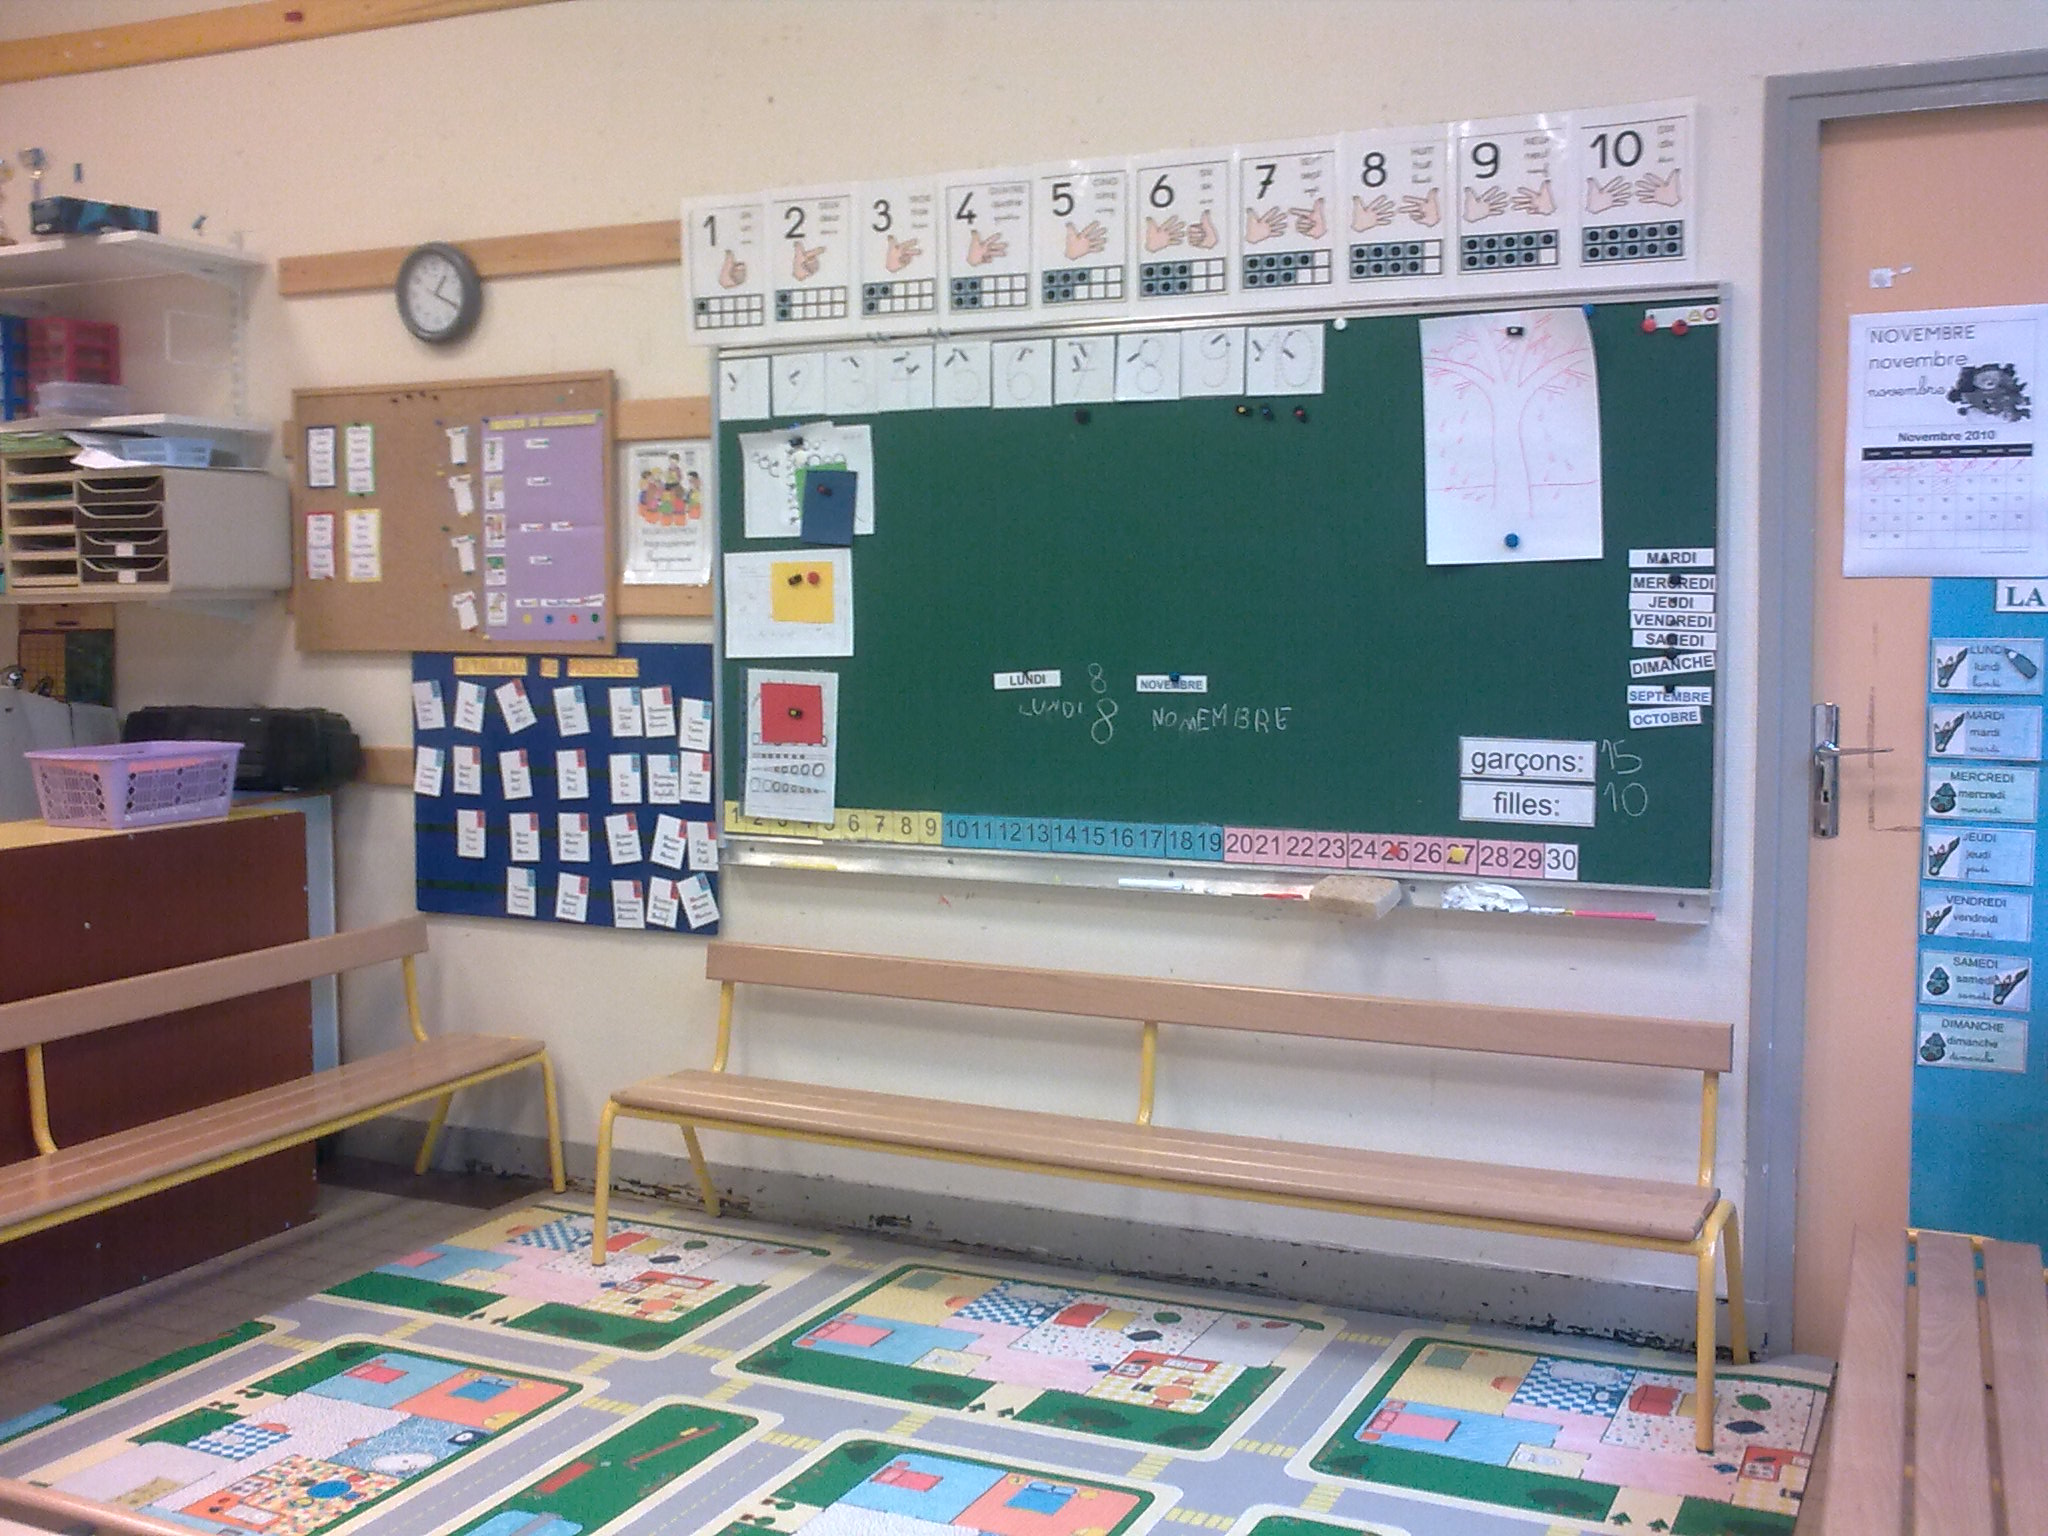
\includegraphics[height = 0.35\textheight]{./fotky/Obr1.jpg}
		\caption{
			Tabule s návody, číslicemi, datem a pipisem ateliérů a prostor pro raní kruh (viz.~\ref{sec:tridaVybaveni}).
		}
		\label{Obr1}
	\end{figure}

	\begin{figure}[tb]
		\centering
		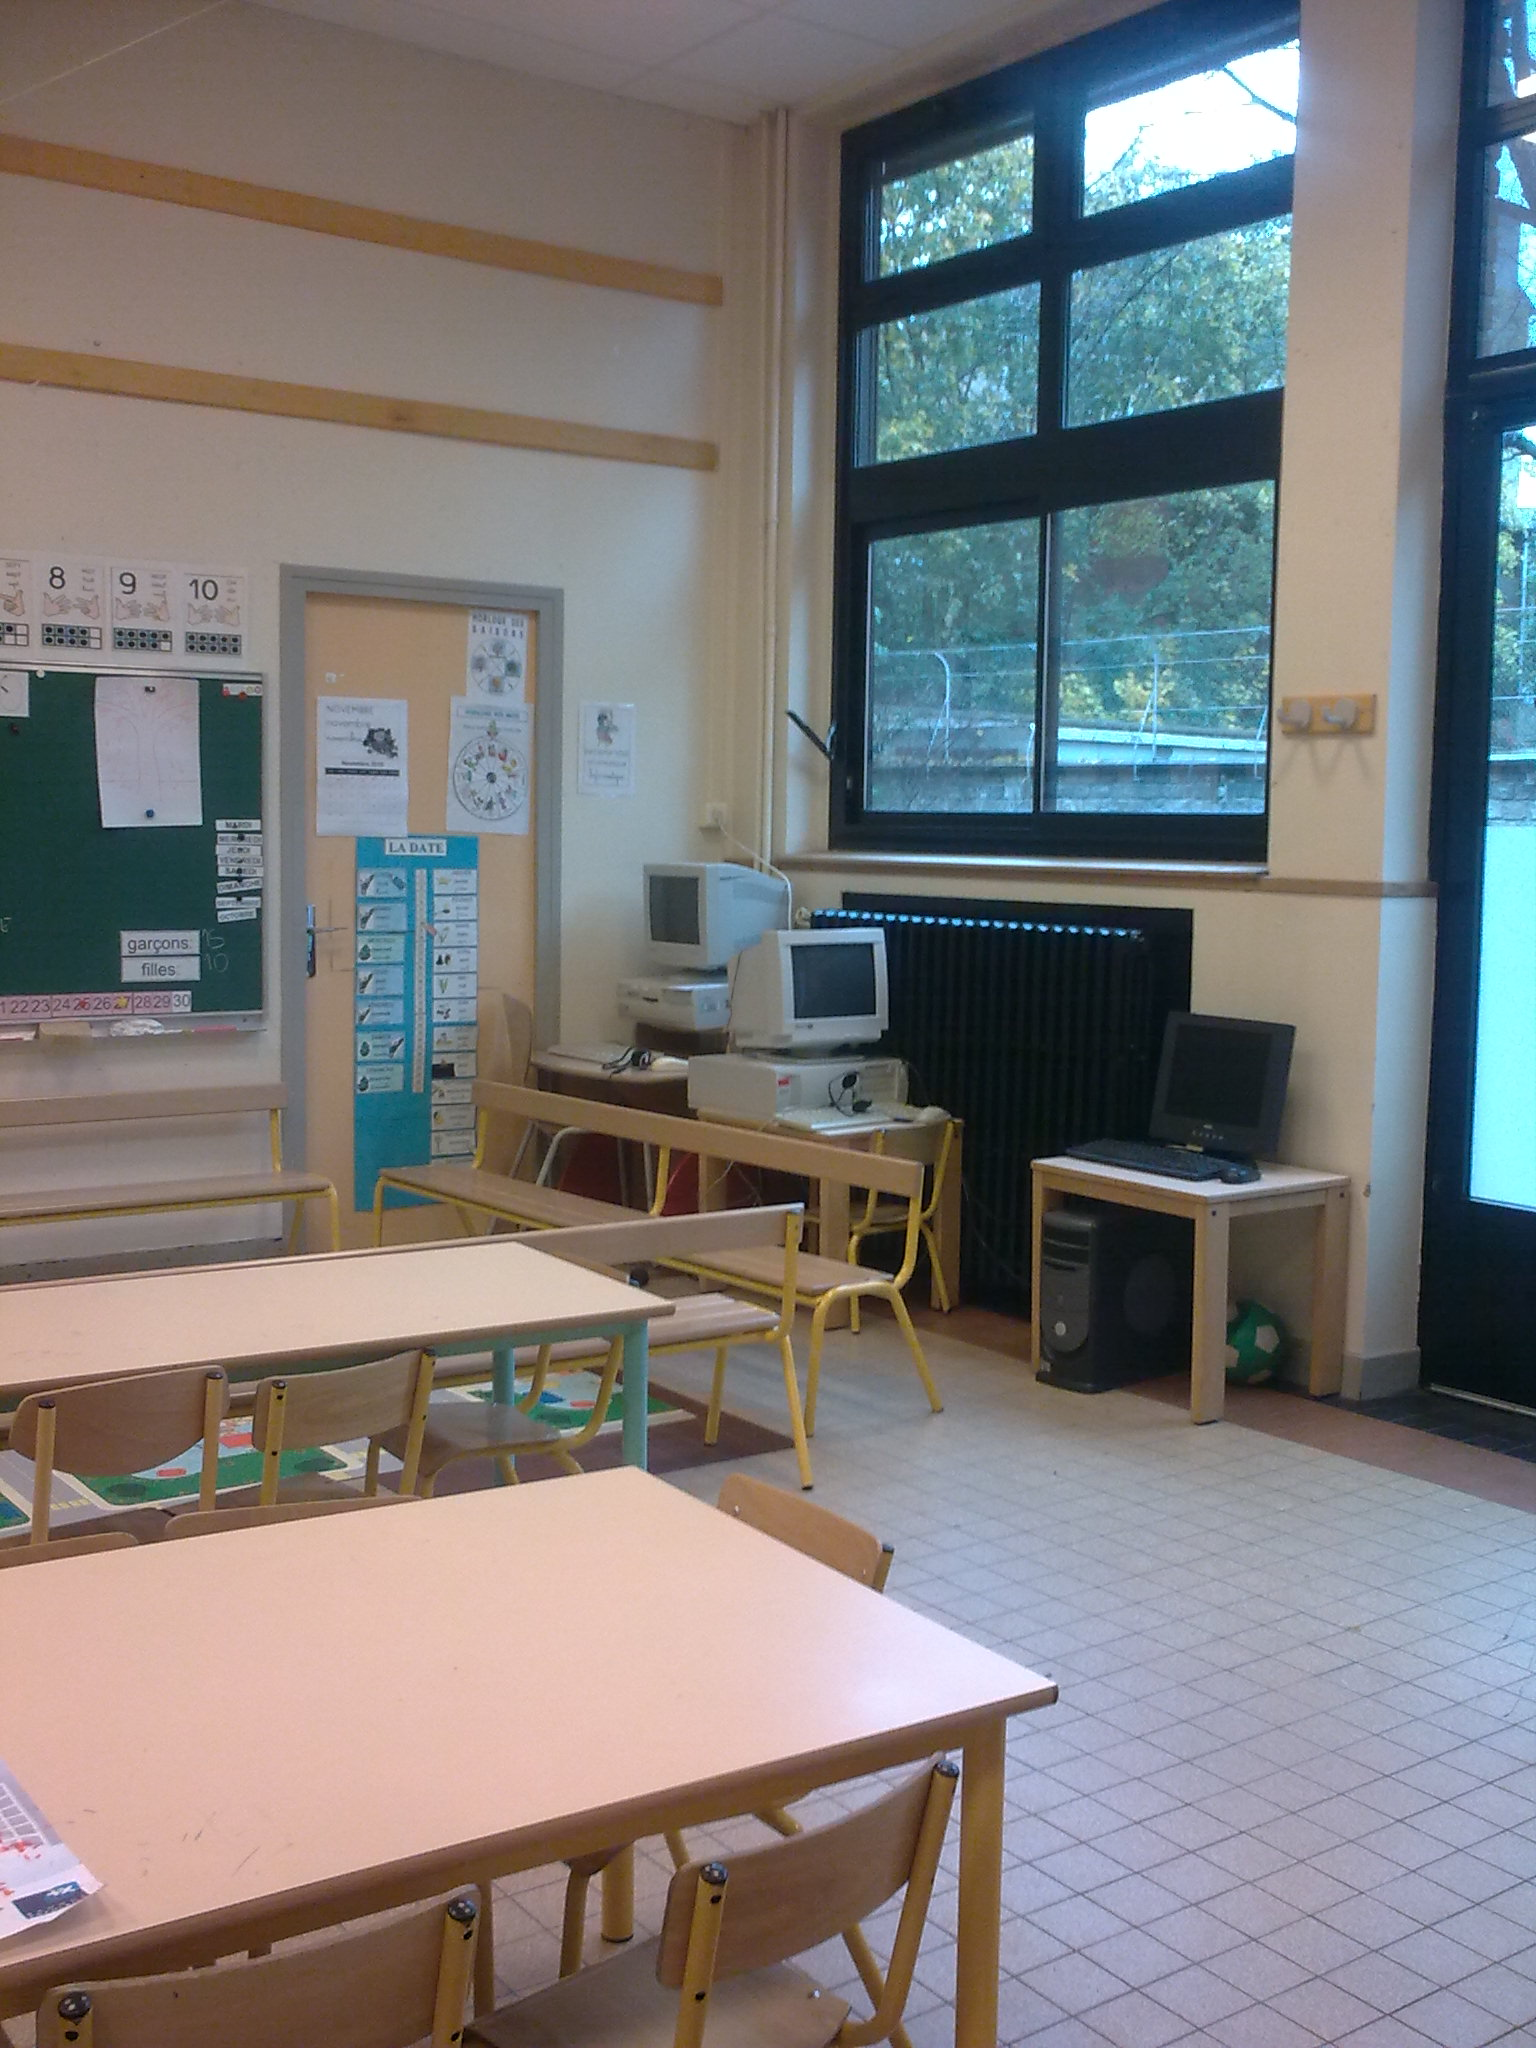
\includegraphics[height = 0.35\textheight]{./fotky/Obr2.jpg}
		\caption{
			Stolky s počítači a vchod na dvůr (viz.~\ref{sec:tridaVybaveni}).
		}
		\label{Obr2}
	\end{figure}

	\begin{figure}[tb]
		\centering
		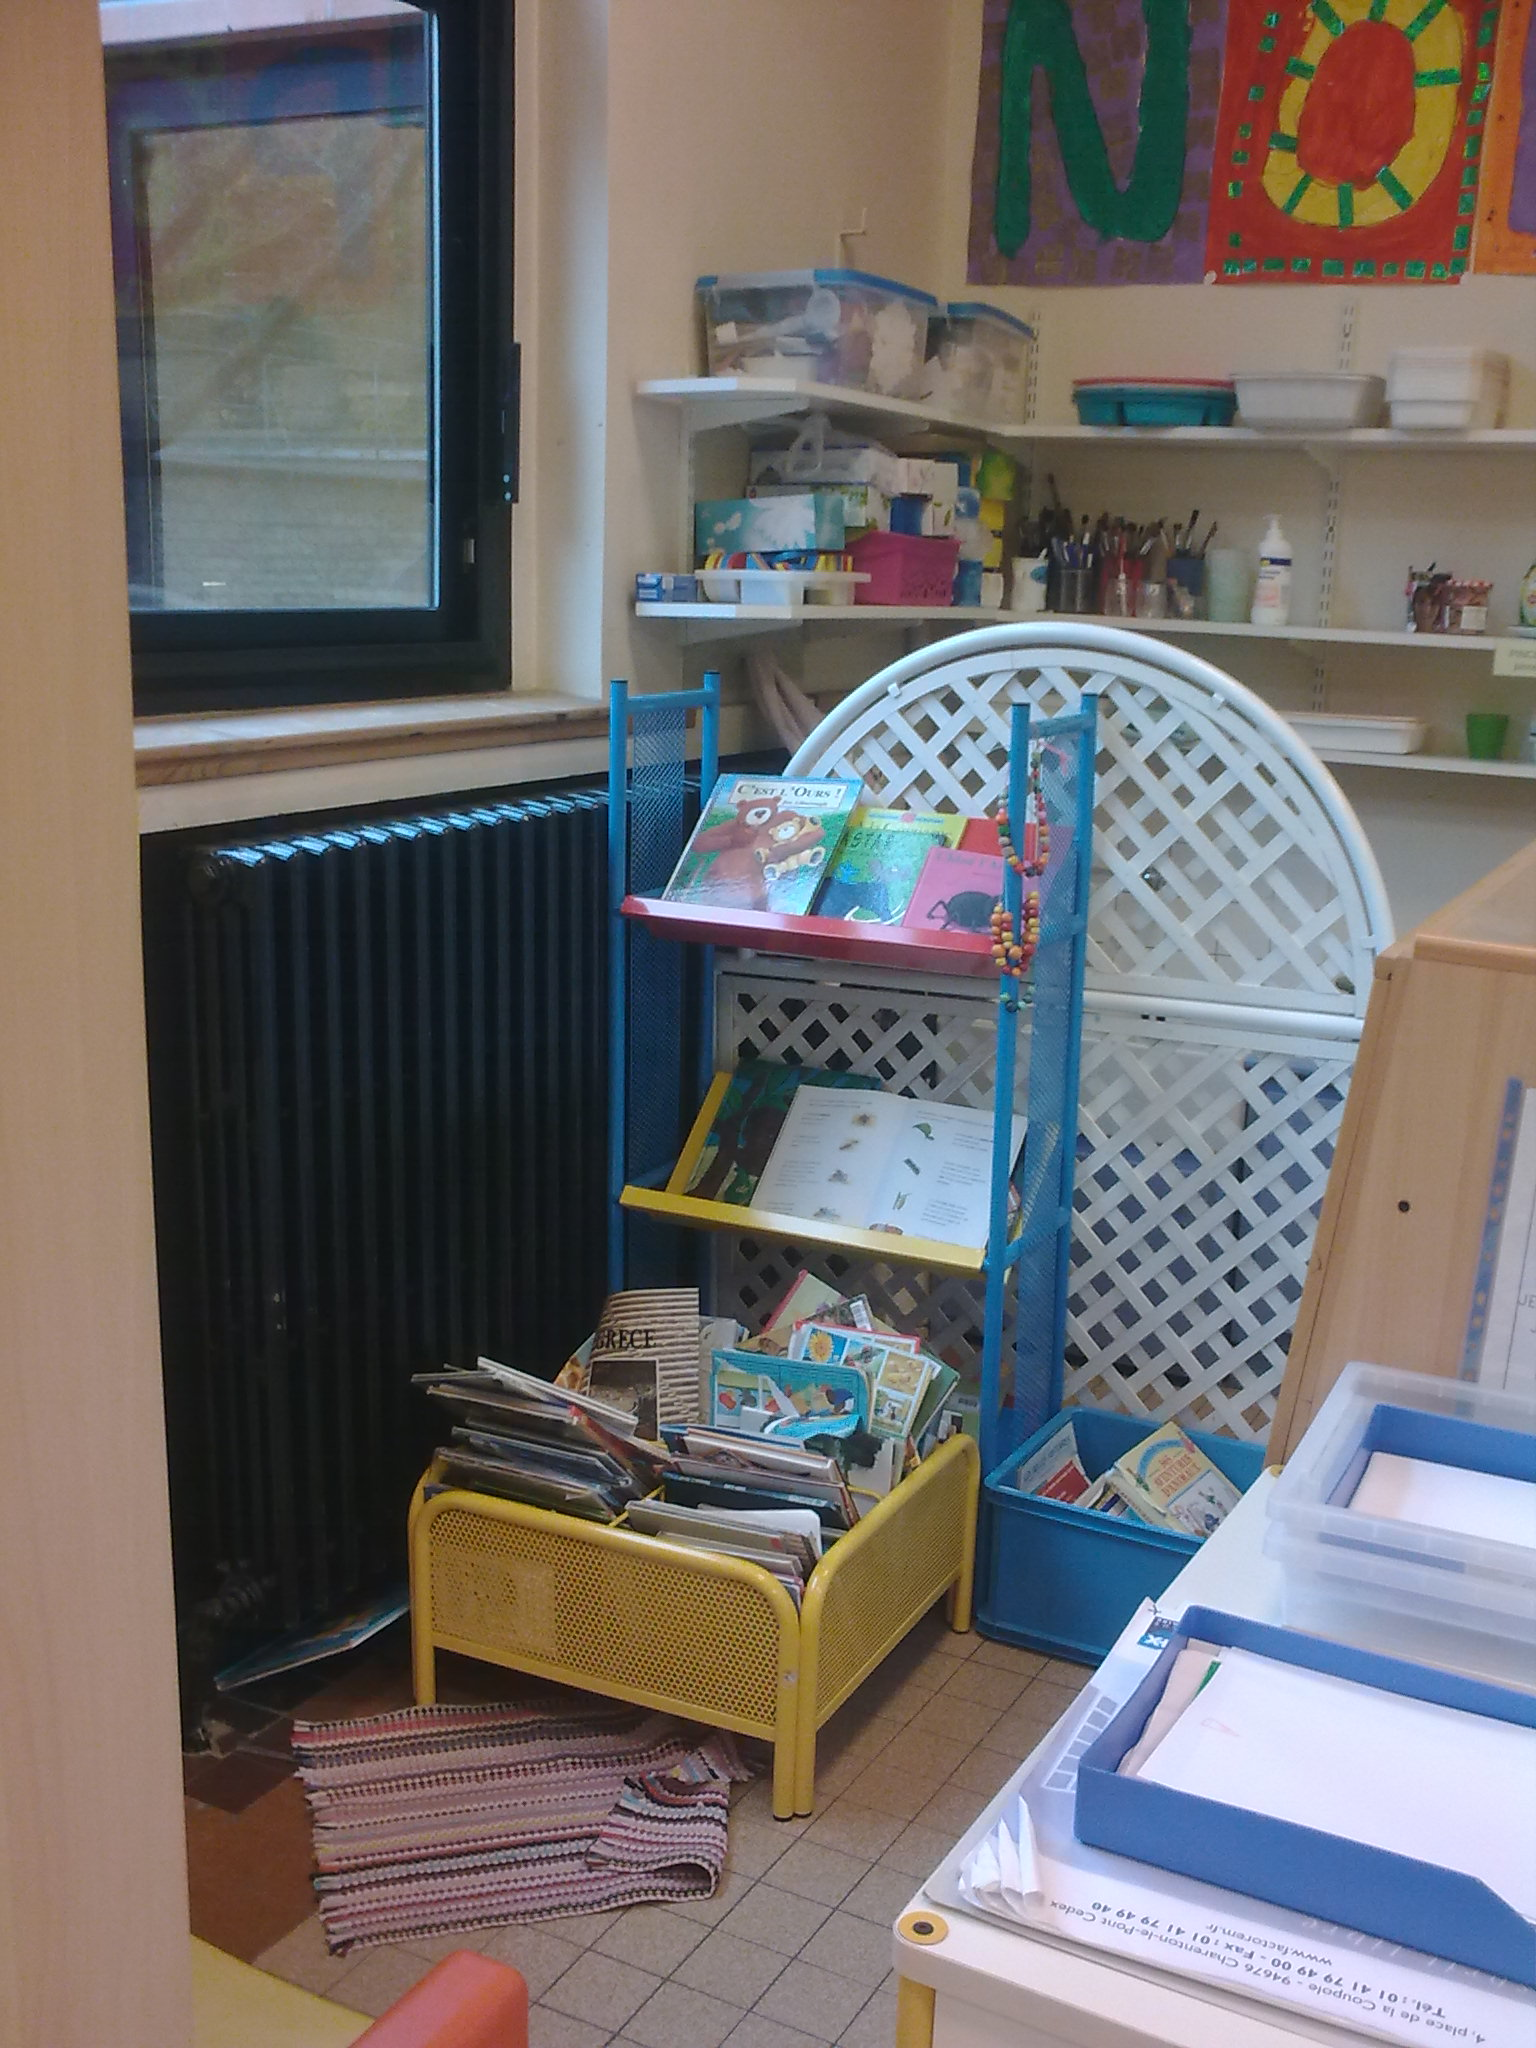
\includegraphics[height = 0.35\textheight]{./fotky/Obr3.jpg}
		\caption{
			Literární koutek s křesílkem (viz.~\ref{sec:tridaVybaveni}).
		}
		\label{Obr3}
	\end{figure}

	\begin{figure}[tb]
		\centering
		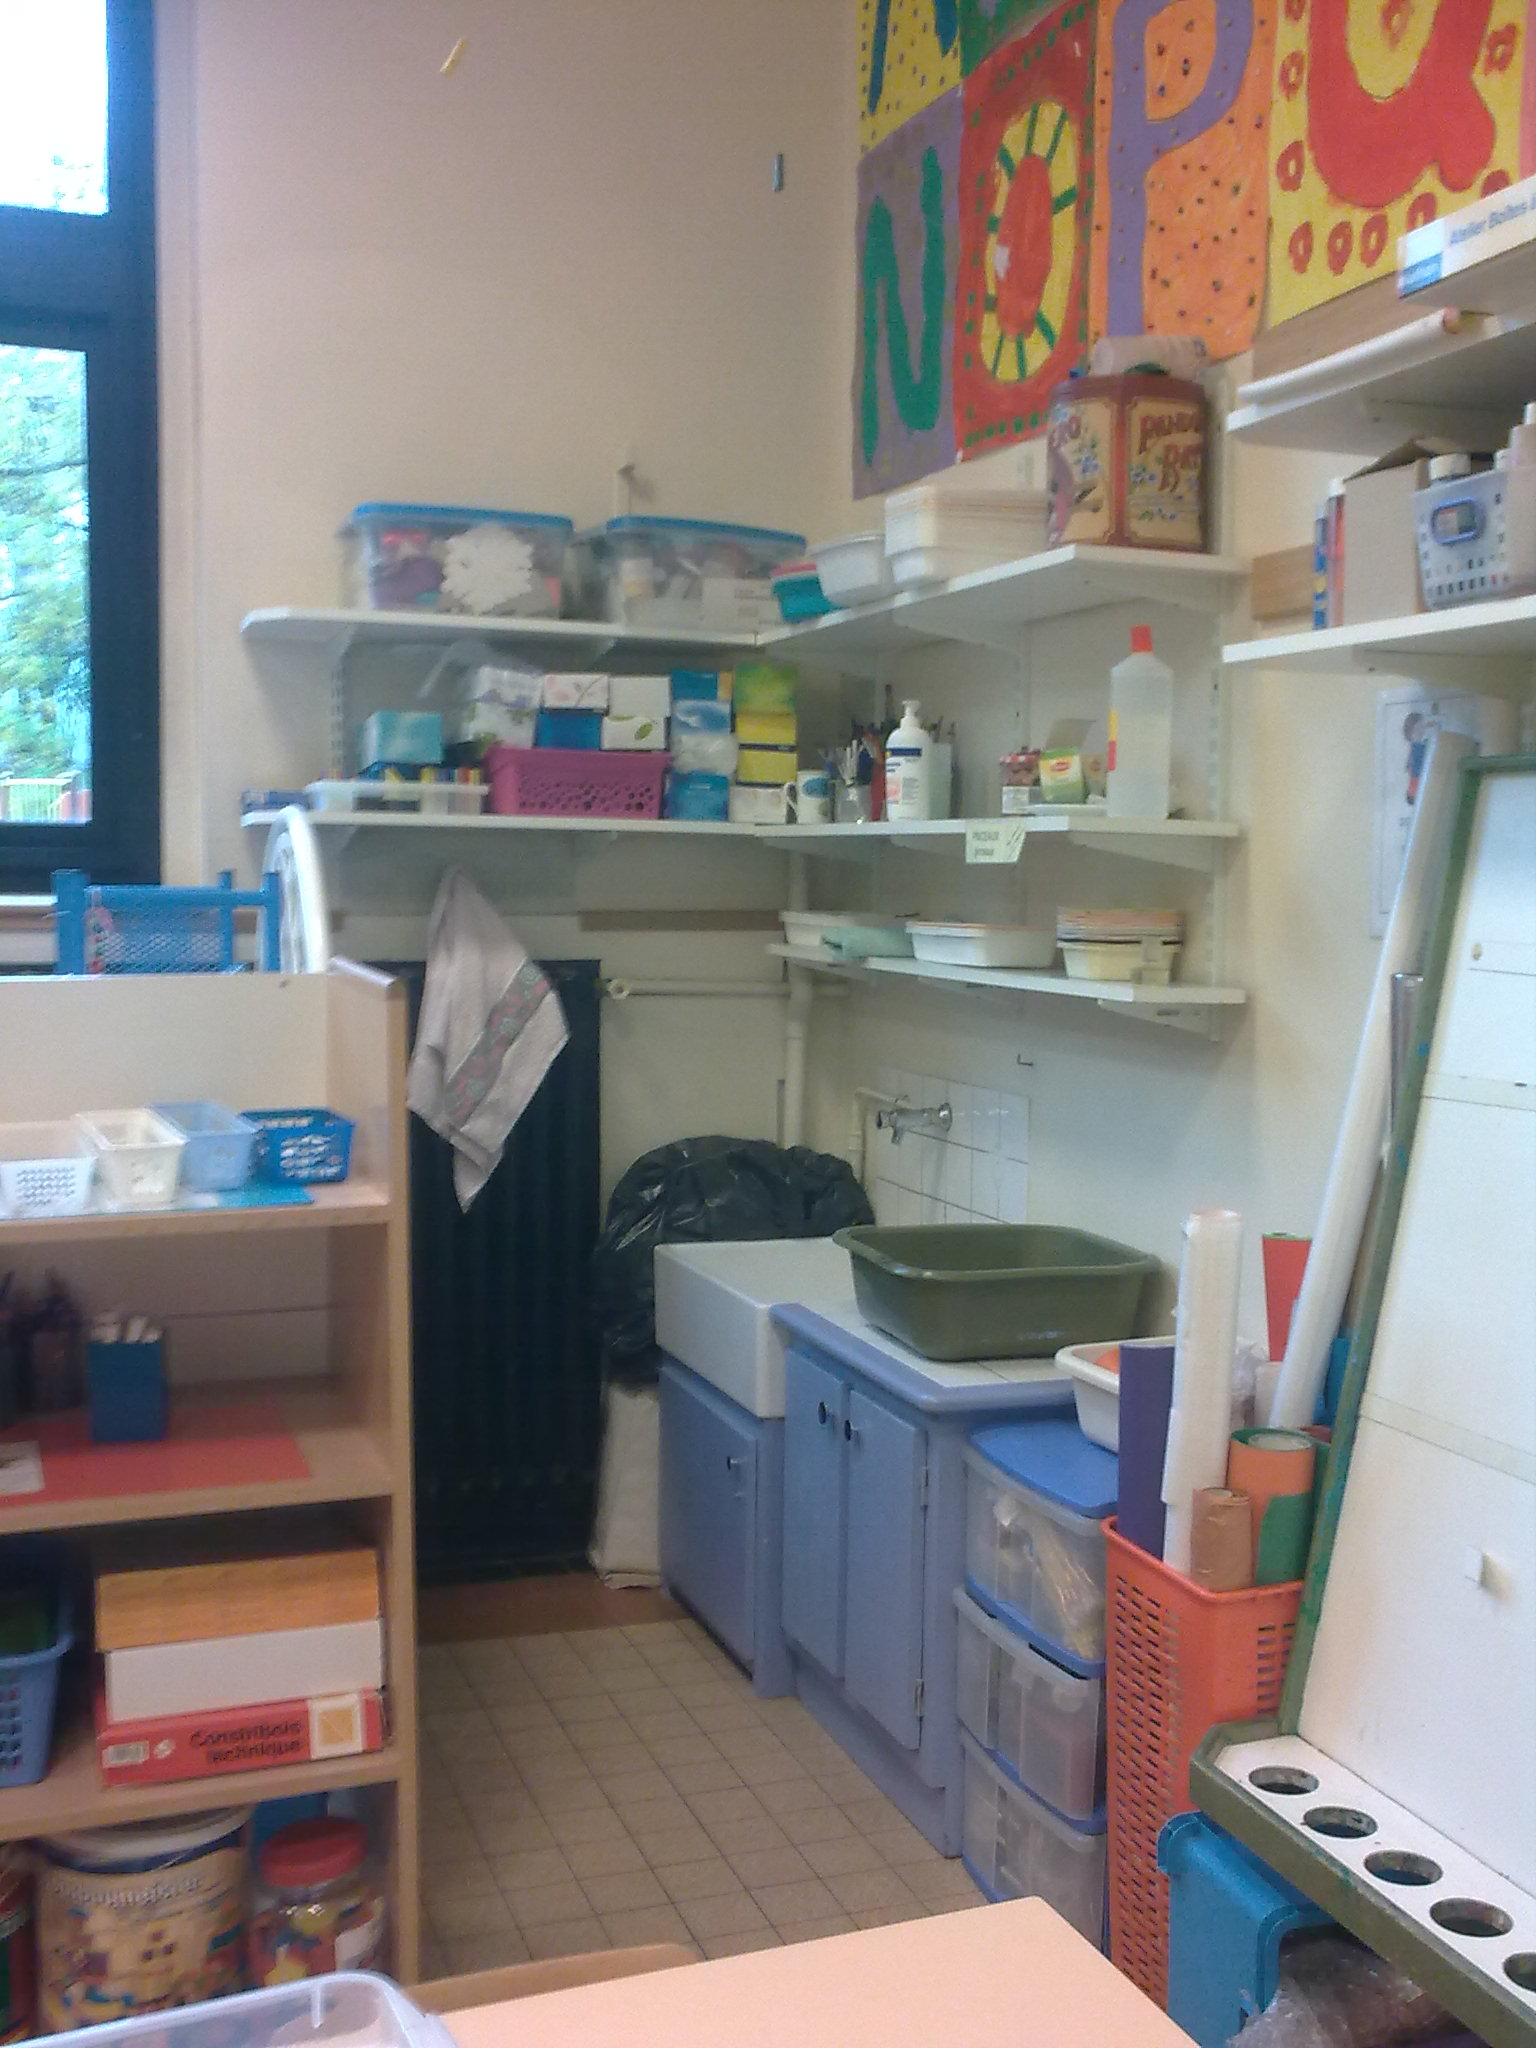
\includegraphics[height = 0.35\textheight]{./fotky/Obr4.jpg}
		\caption{
			Umyvadlo a police na materiál (viz.~\ref{sec:tridaVybaveni}).
		}
		\label{Obr4}
	\end{figure}

	\begin{figure}[tb]
		\centering
		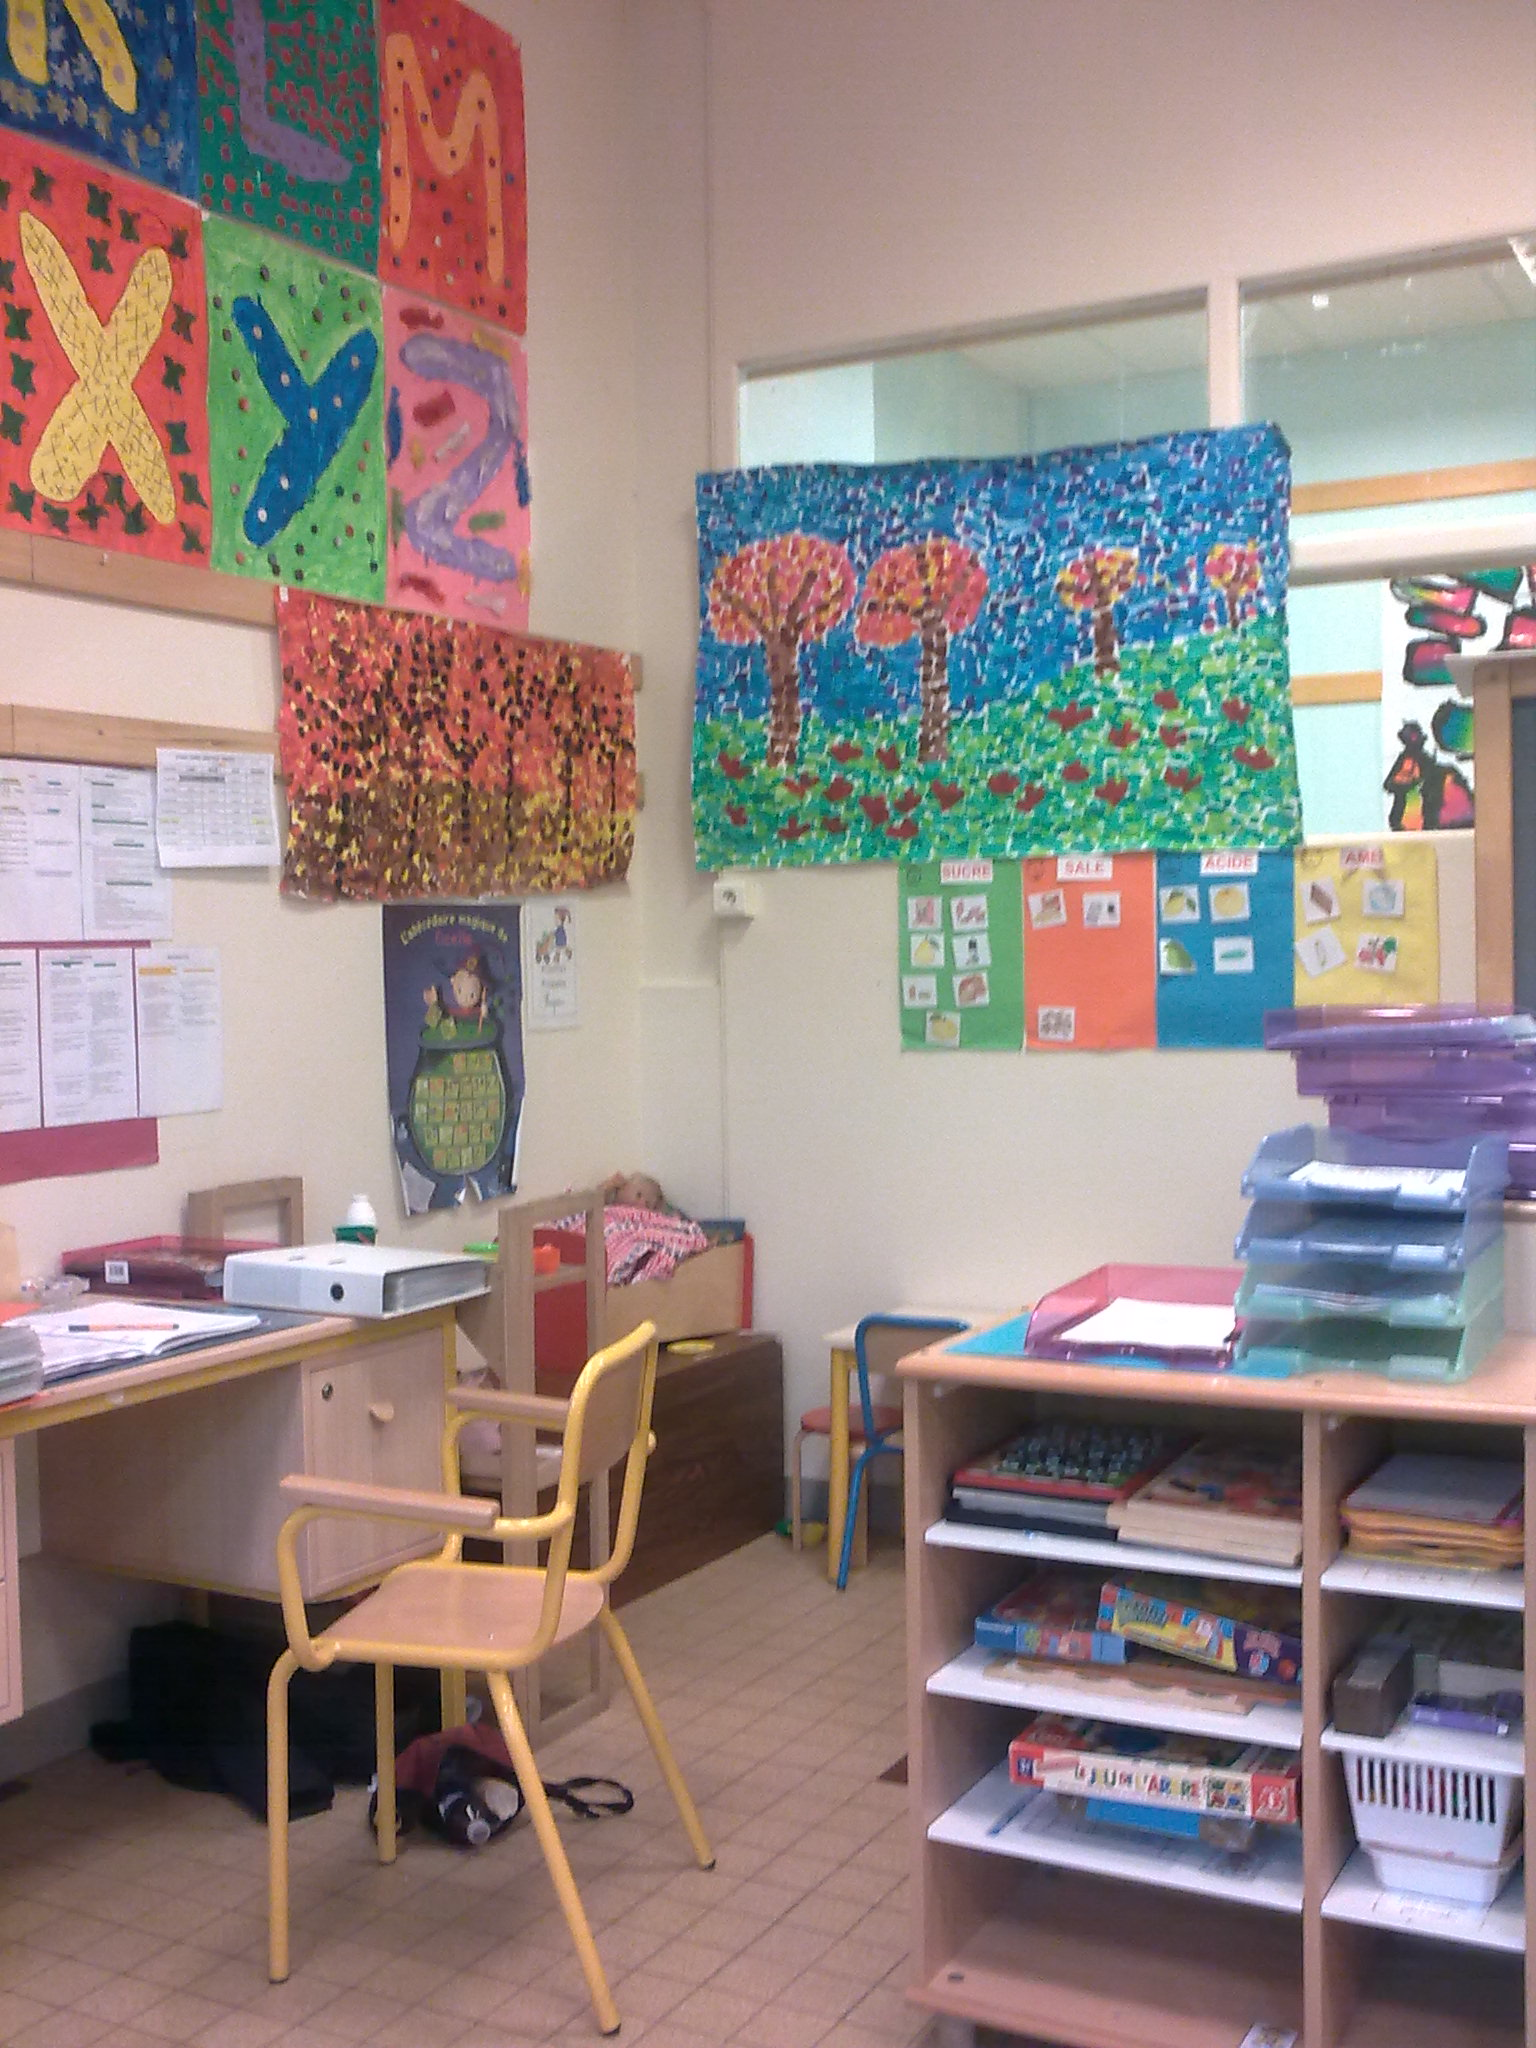
\includegraphics[height = 0.35\textheight]{./fotky/Obr5.jpg}
		\caption{
			Stůl pro učitelku, dětská kuchyňka a poličky na didaktické pomůcky kecy (viz.~\ref{sec:tridaVybaveni}).
		}
		\label{Obr5}
	\end{figure}

	\begin{figure}[tb]
		\centering
		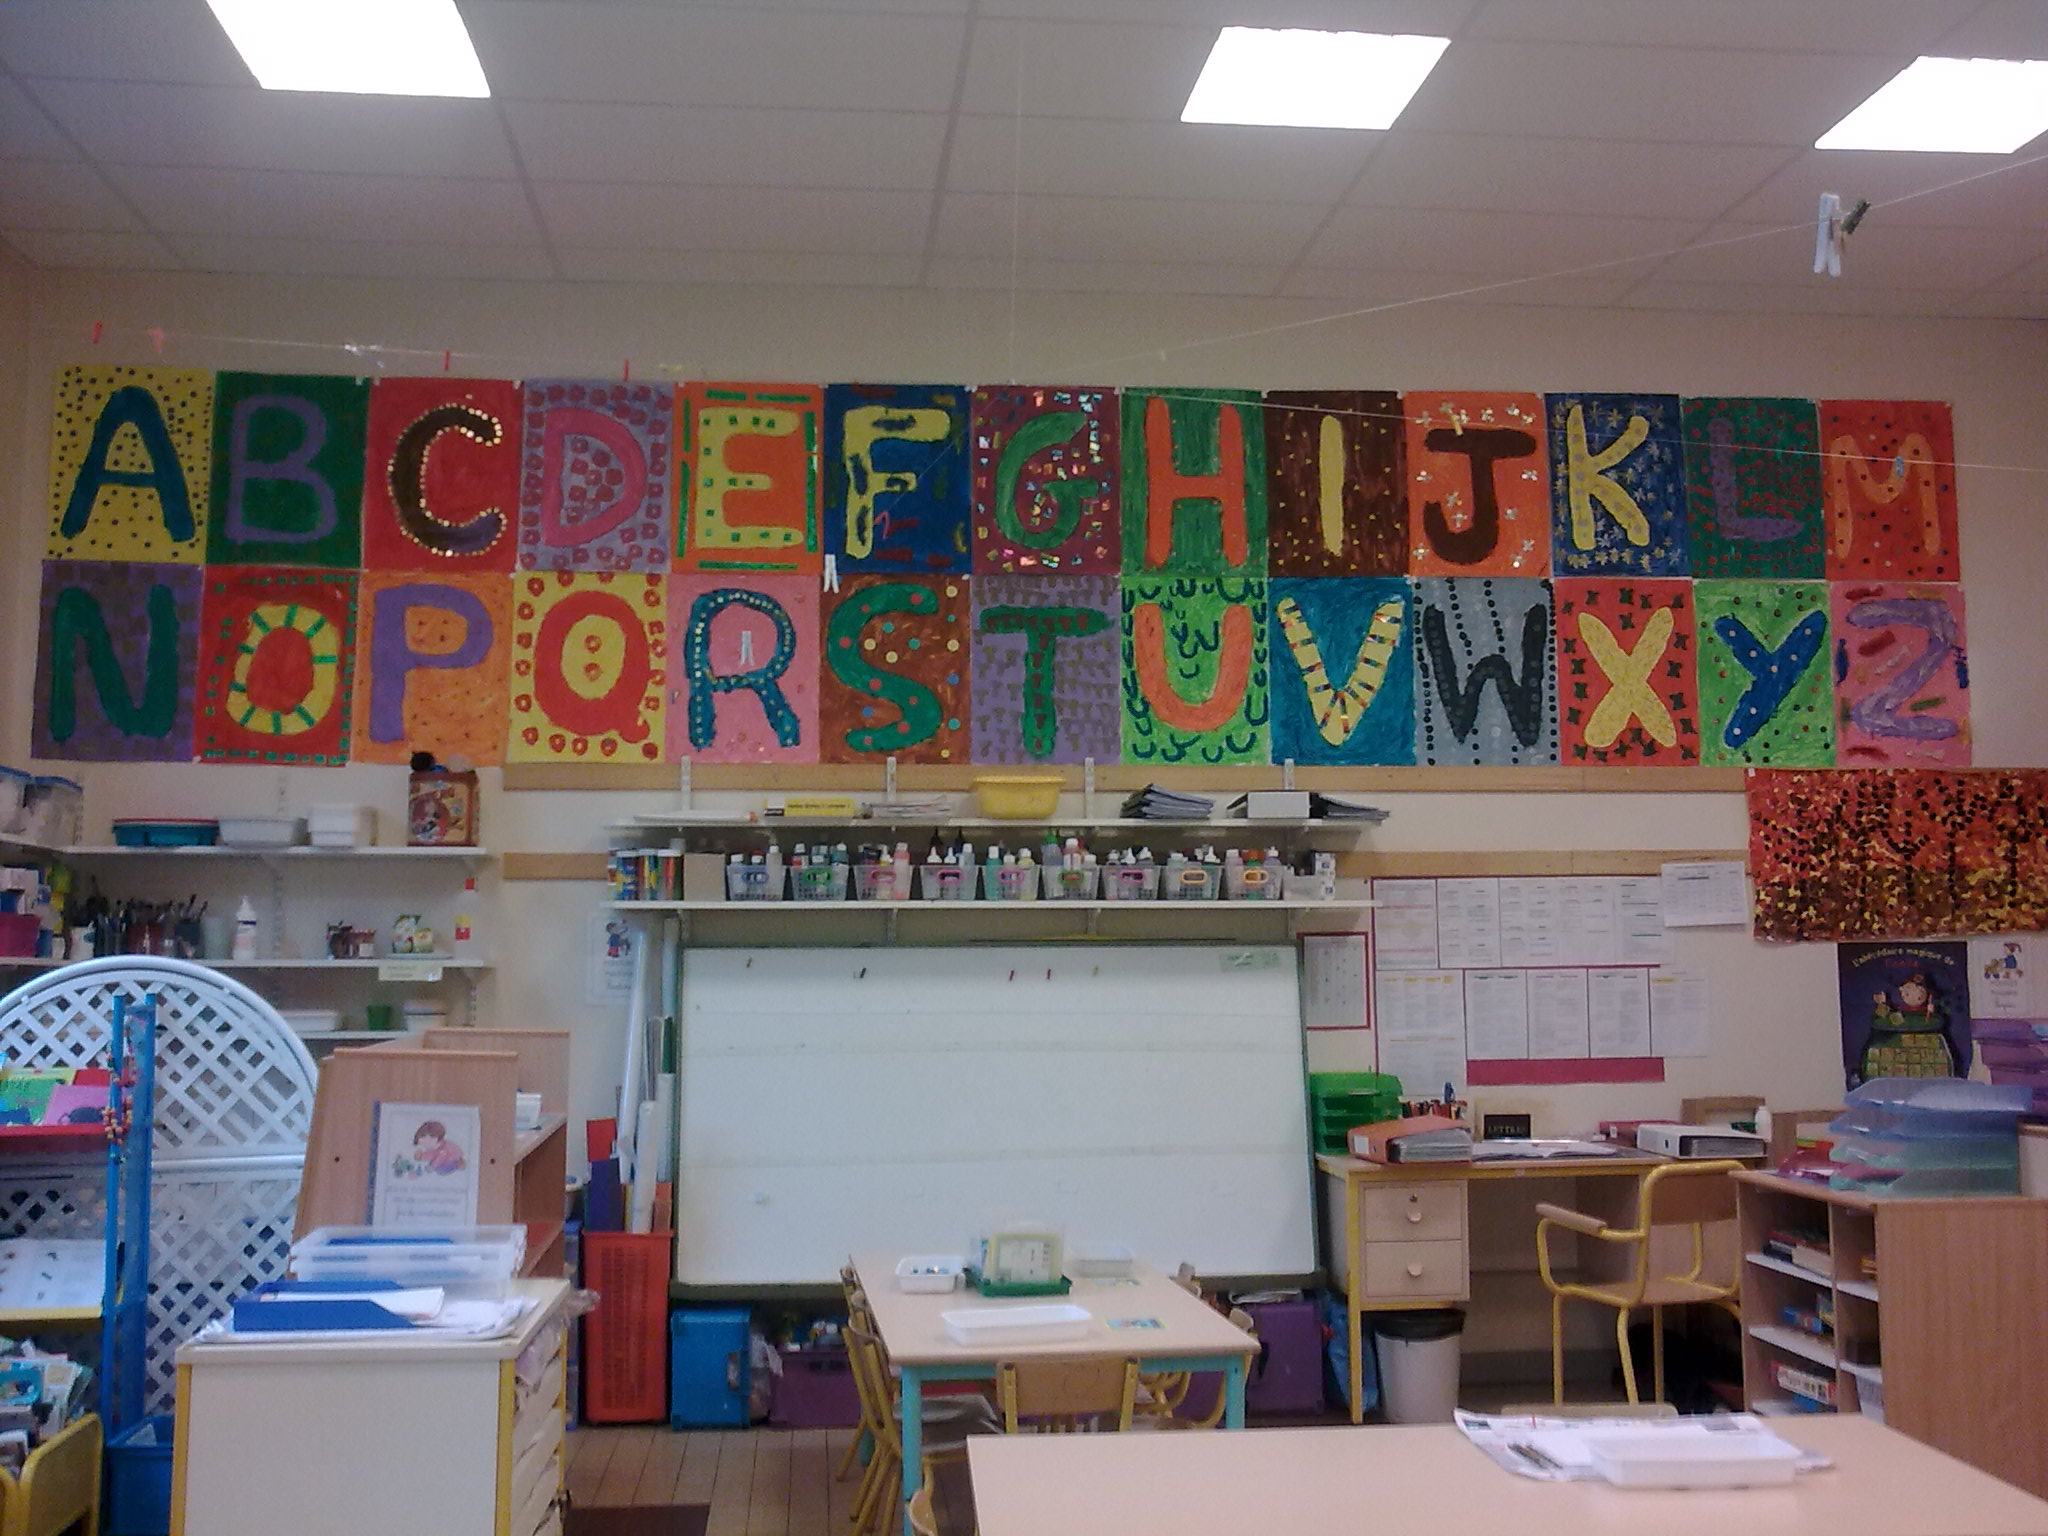
\includegraphics[height = 0.35\textheight]{./fotky/Obr6.jpg}
		\caption{
			Výzdoba třídy písmeny abecedy a pohled na druhou polovinu třídy (viz.~\ref{sec:tridaVybaveni}).
		}
		\label{Obr6}
	\end{figure}


	\begin{figure}[tb]
		\centering
		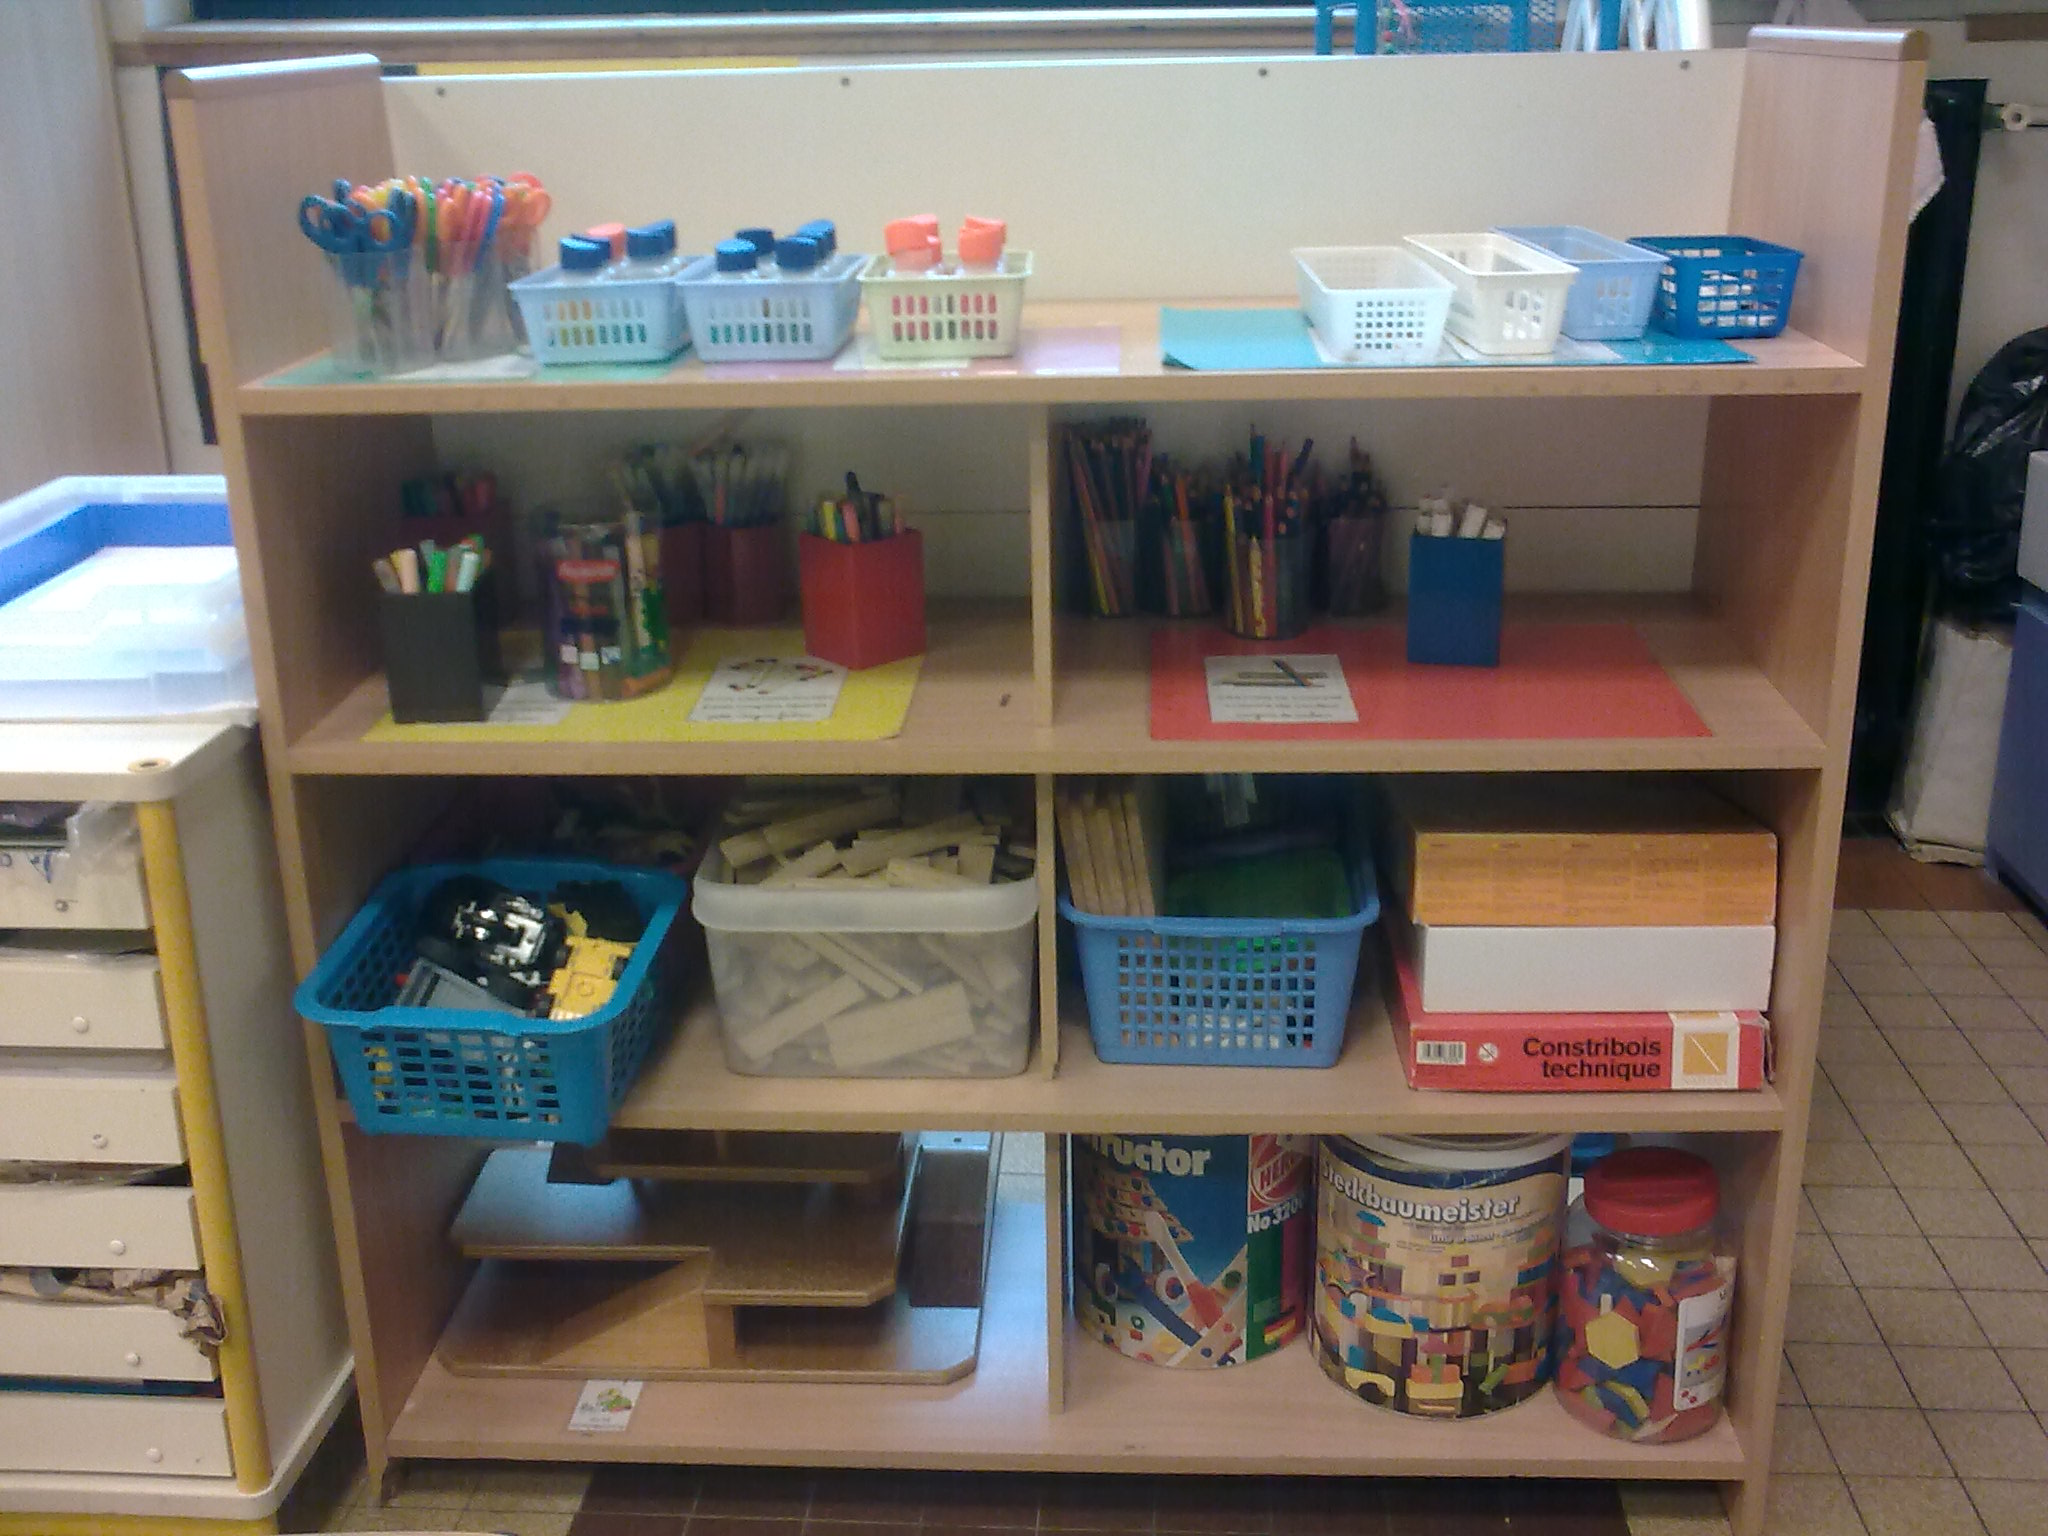
\includegraphics[height = 0.35\textheight]{./fotky/Obr7.jpg}
		\caption{
			Police na materiál a pomůcky (viz.~\ref{sec:tridaVybaveni}).
		}
		\label{Obr7}
	\end{figure}

	\begin{figure}[tb]
		\centering
		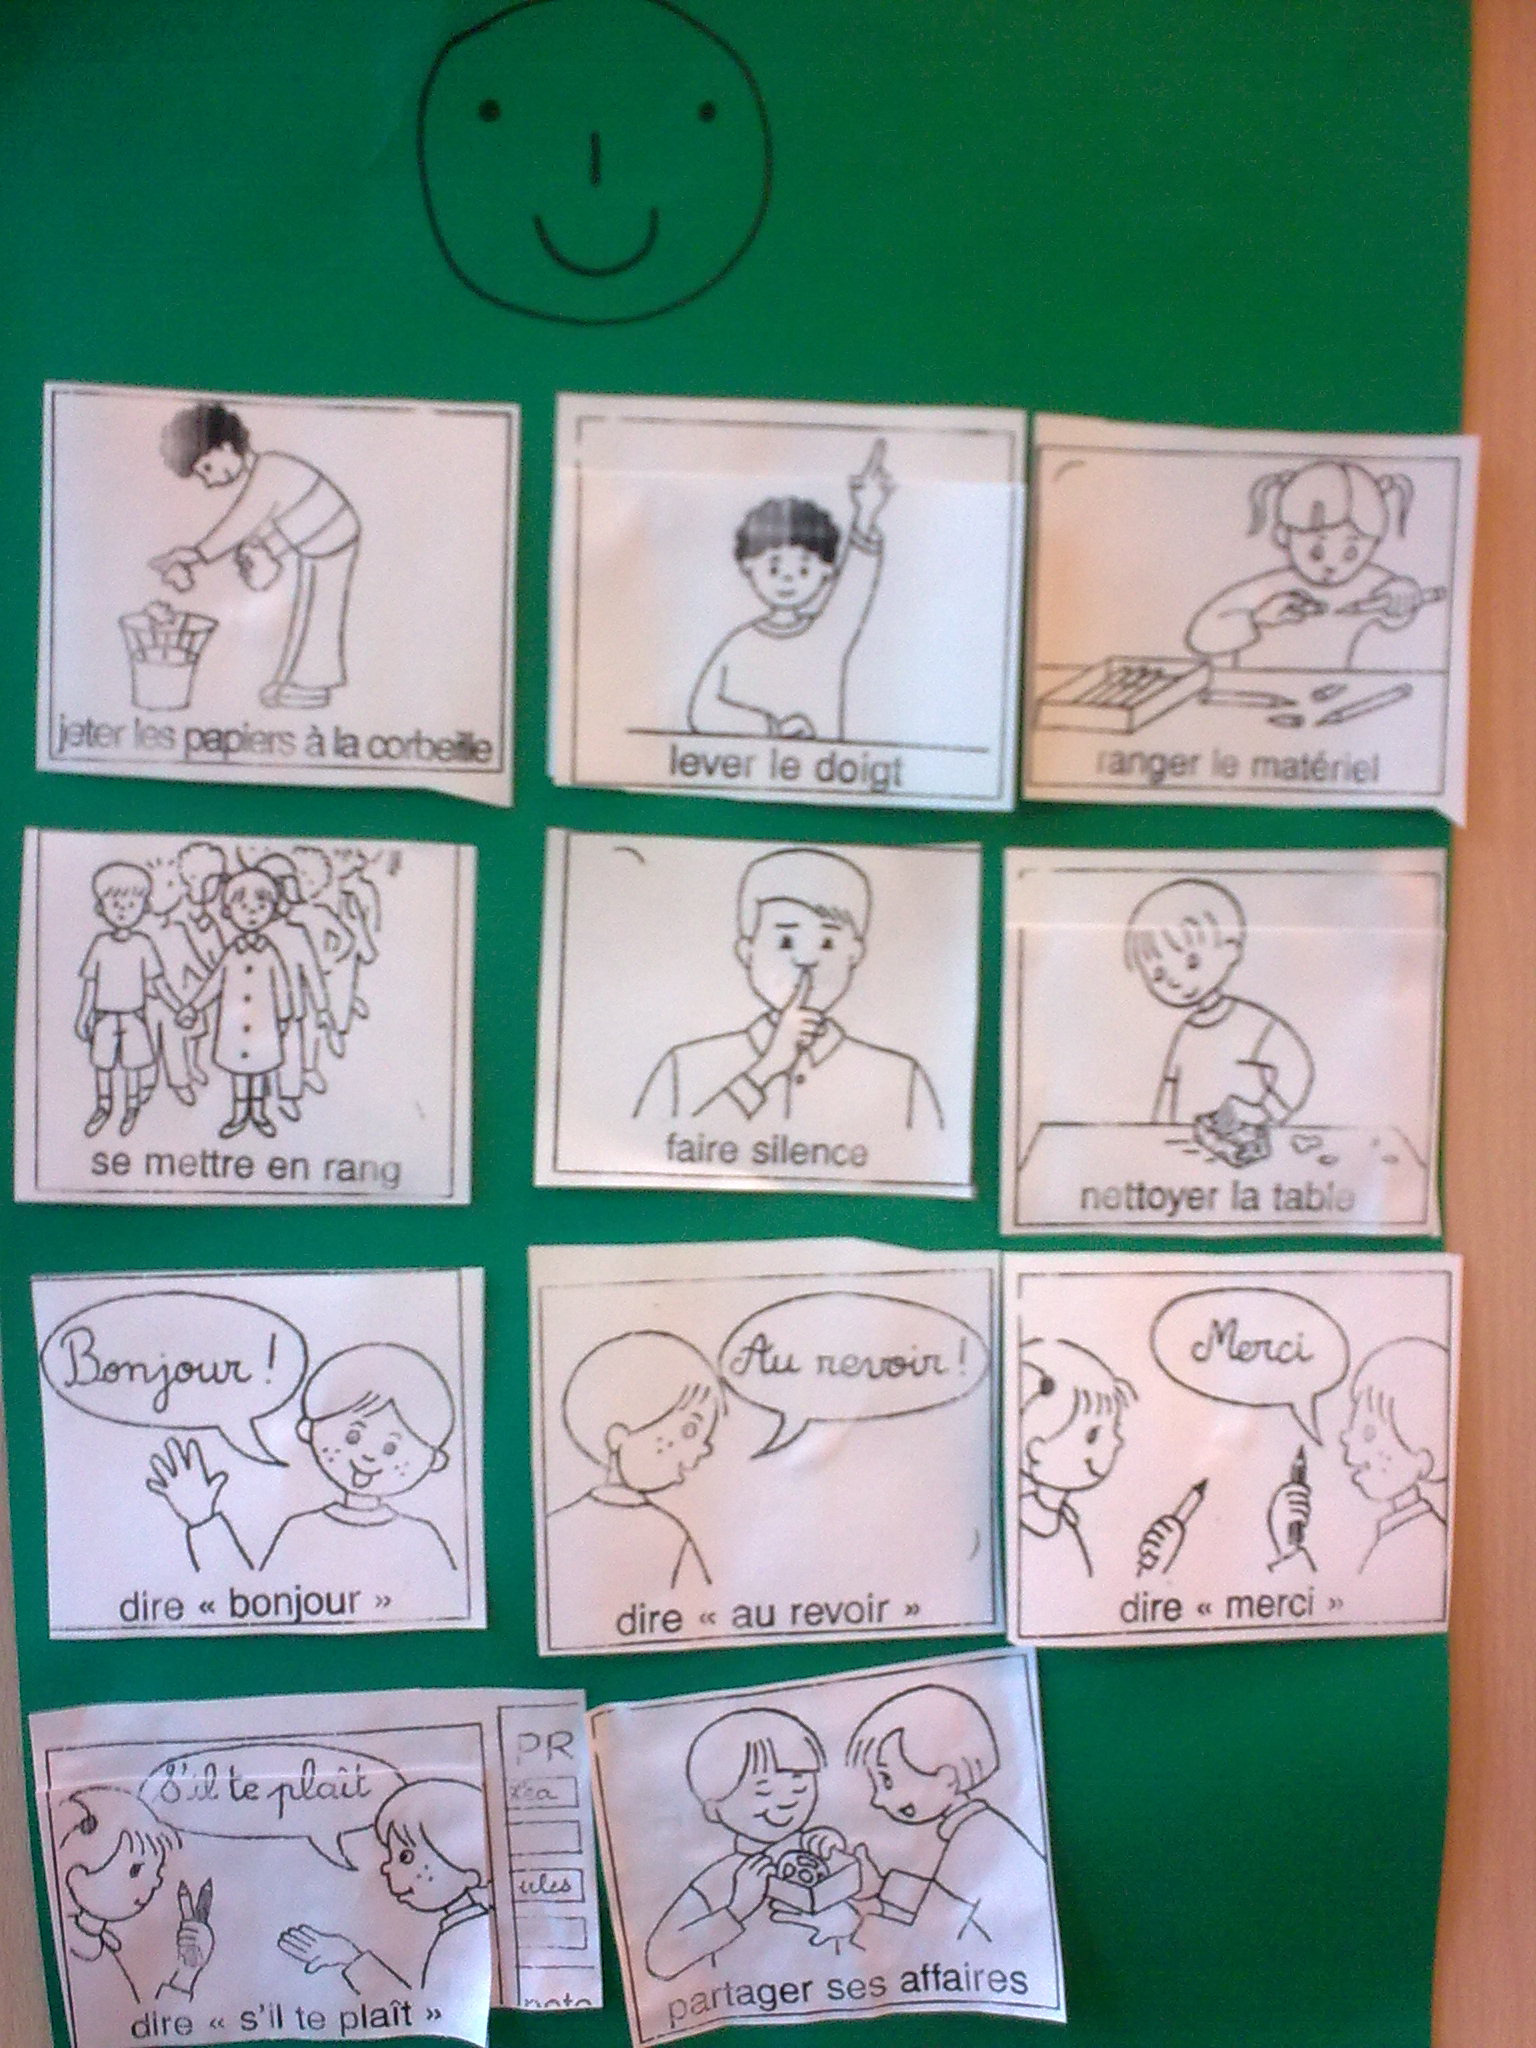
\includegraphics[width = 0.45\linewidth]{./fotky/Obr8a.jpg}
		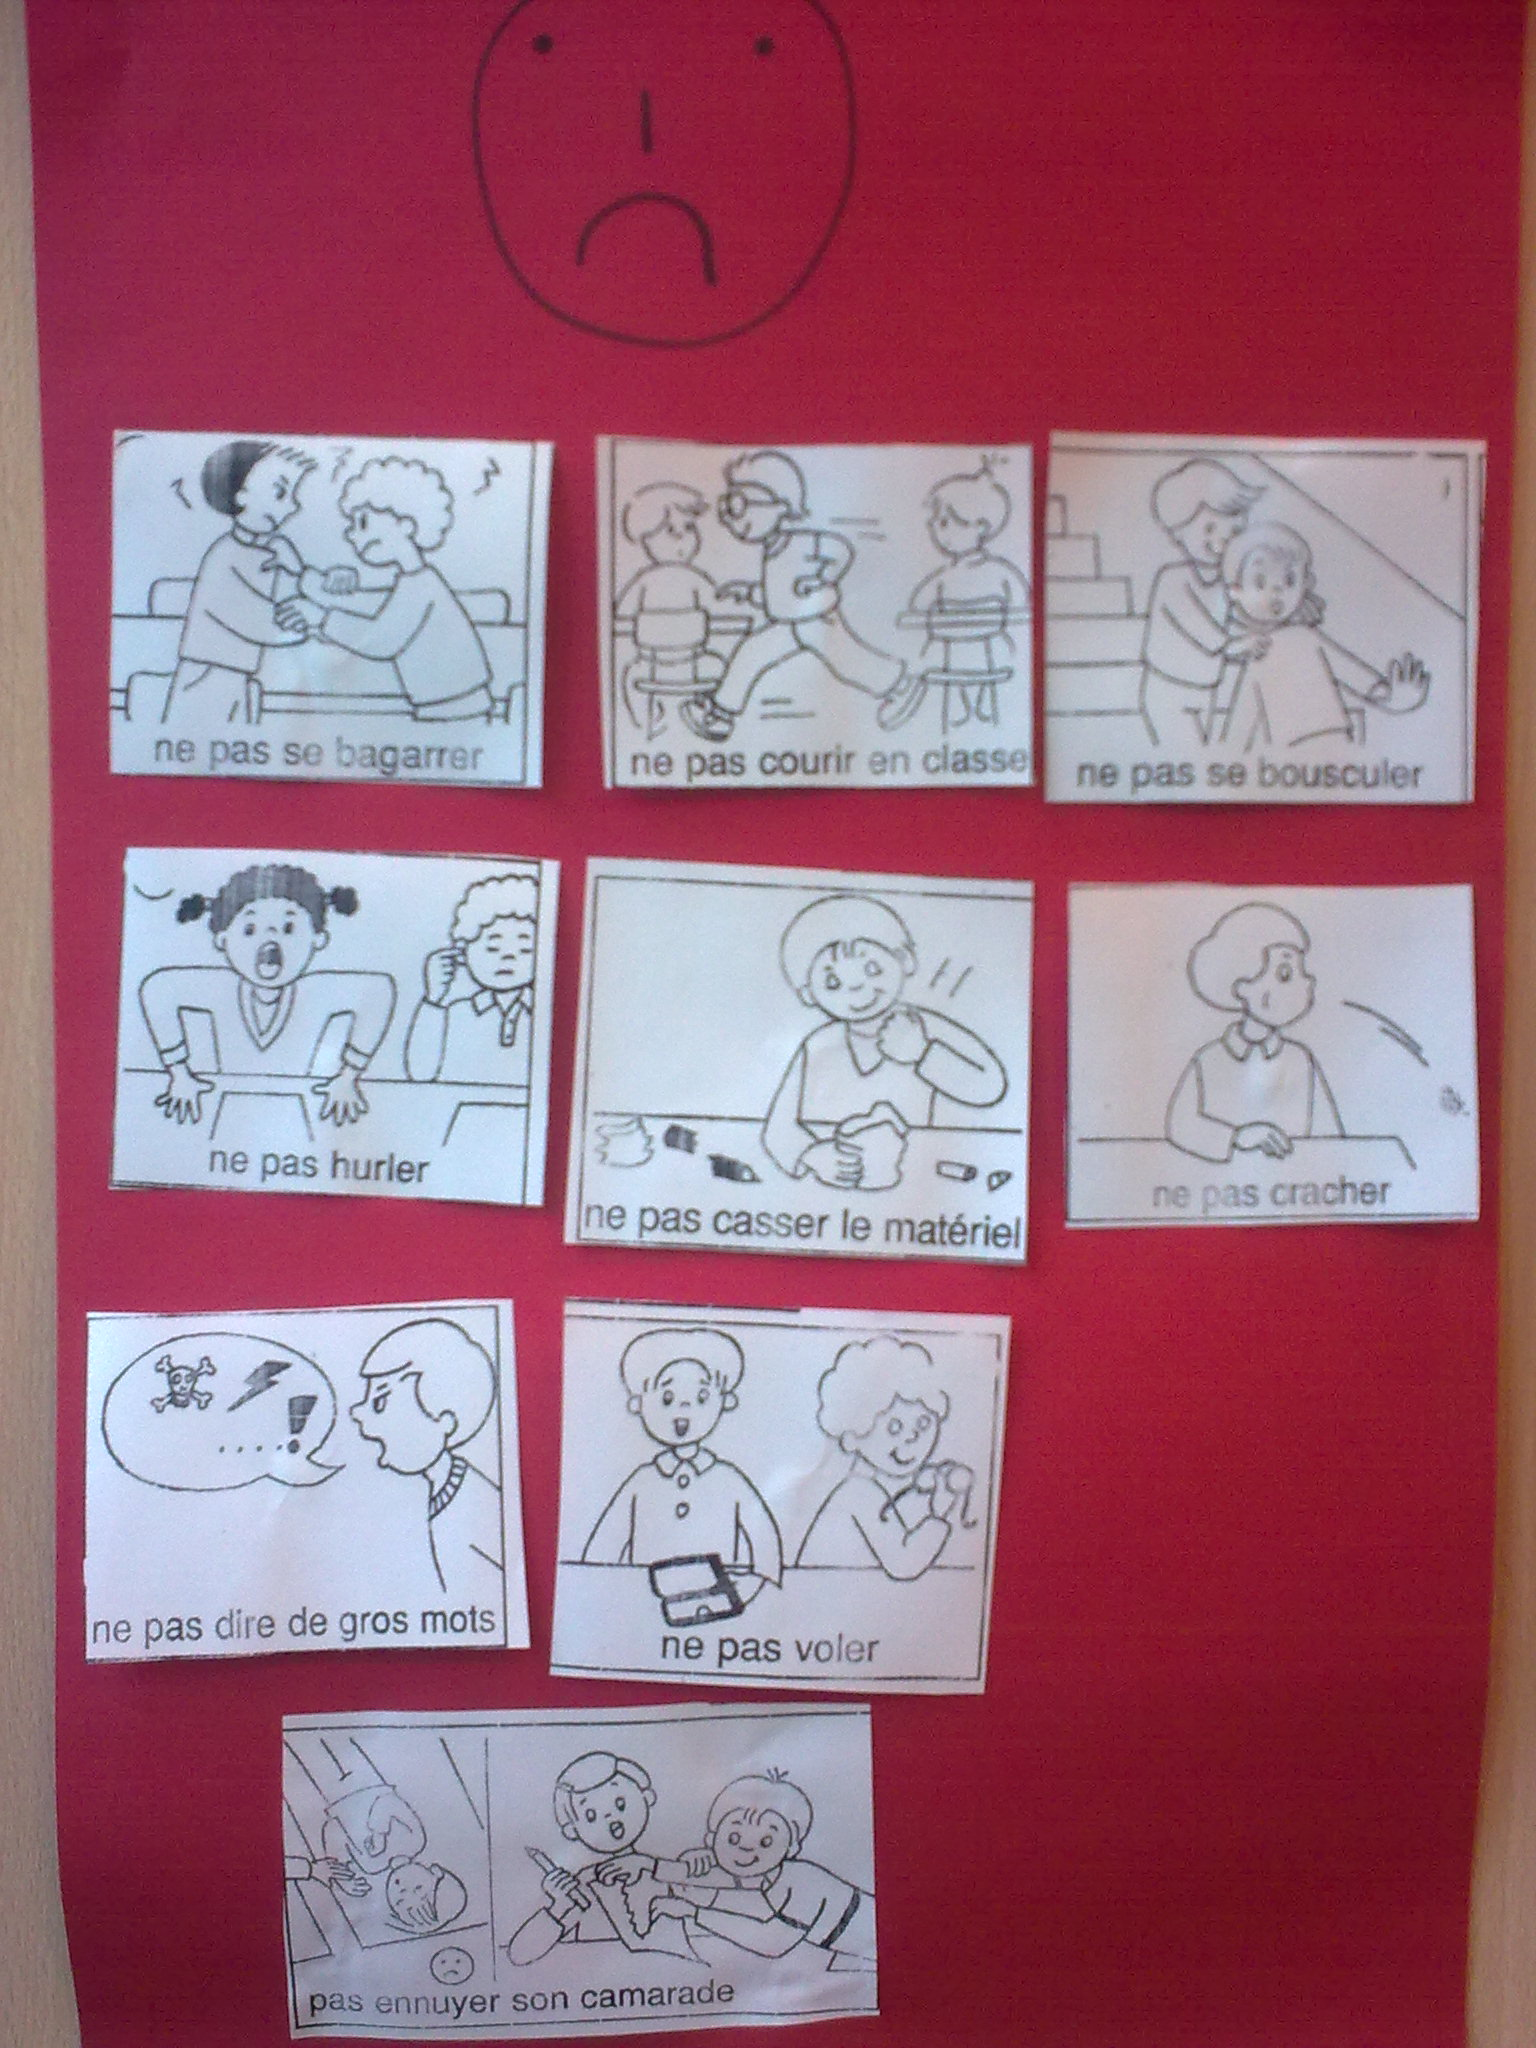
\includegraphics[width = 0.45\linewidth]{./fotky/Obr8b.jpg}
		\caption{
			vyvěšená ravidla třídy (viz.~\ref{pravidlaChovani}).
		}
		\label{Obr8}
	\end{figure}

	\begin{figure}[tb]
		\centering
		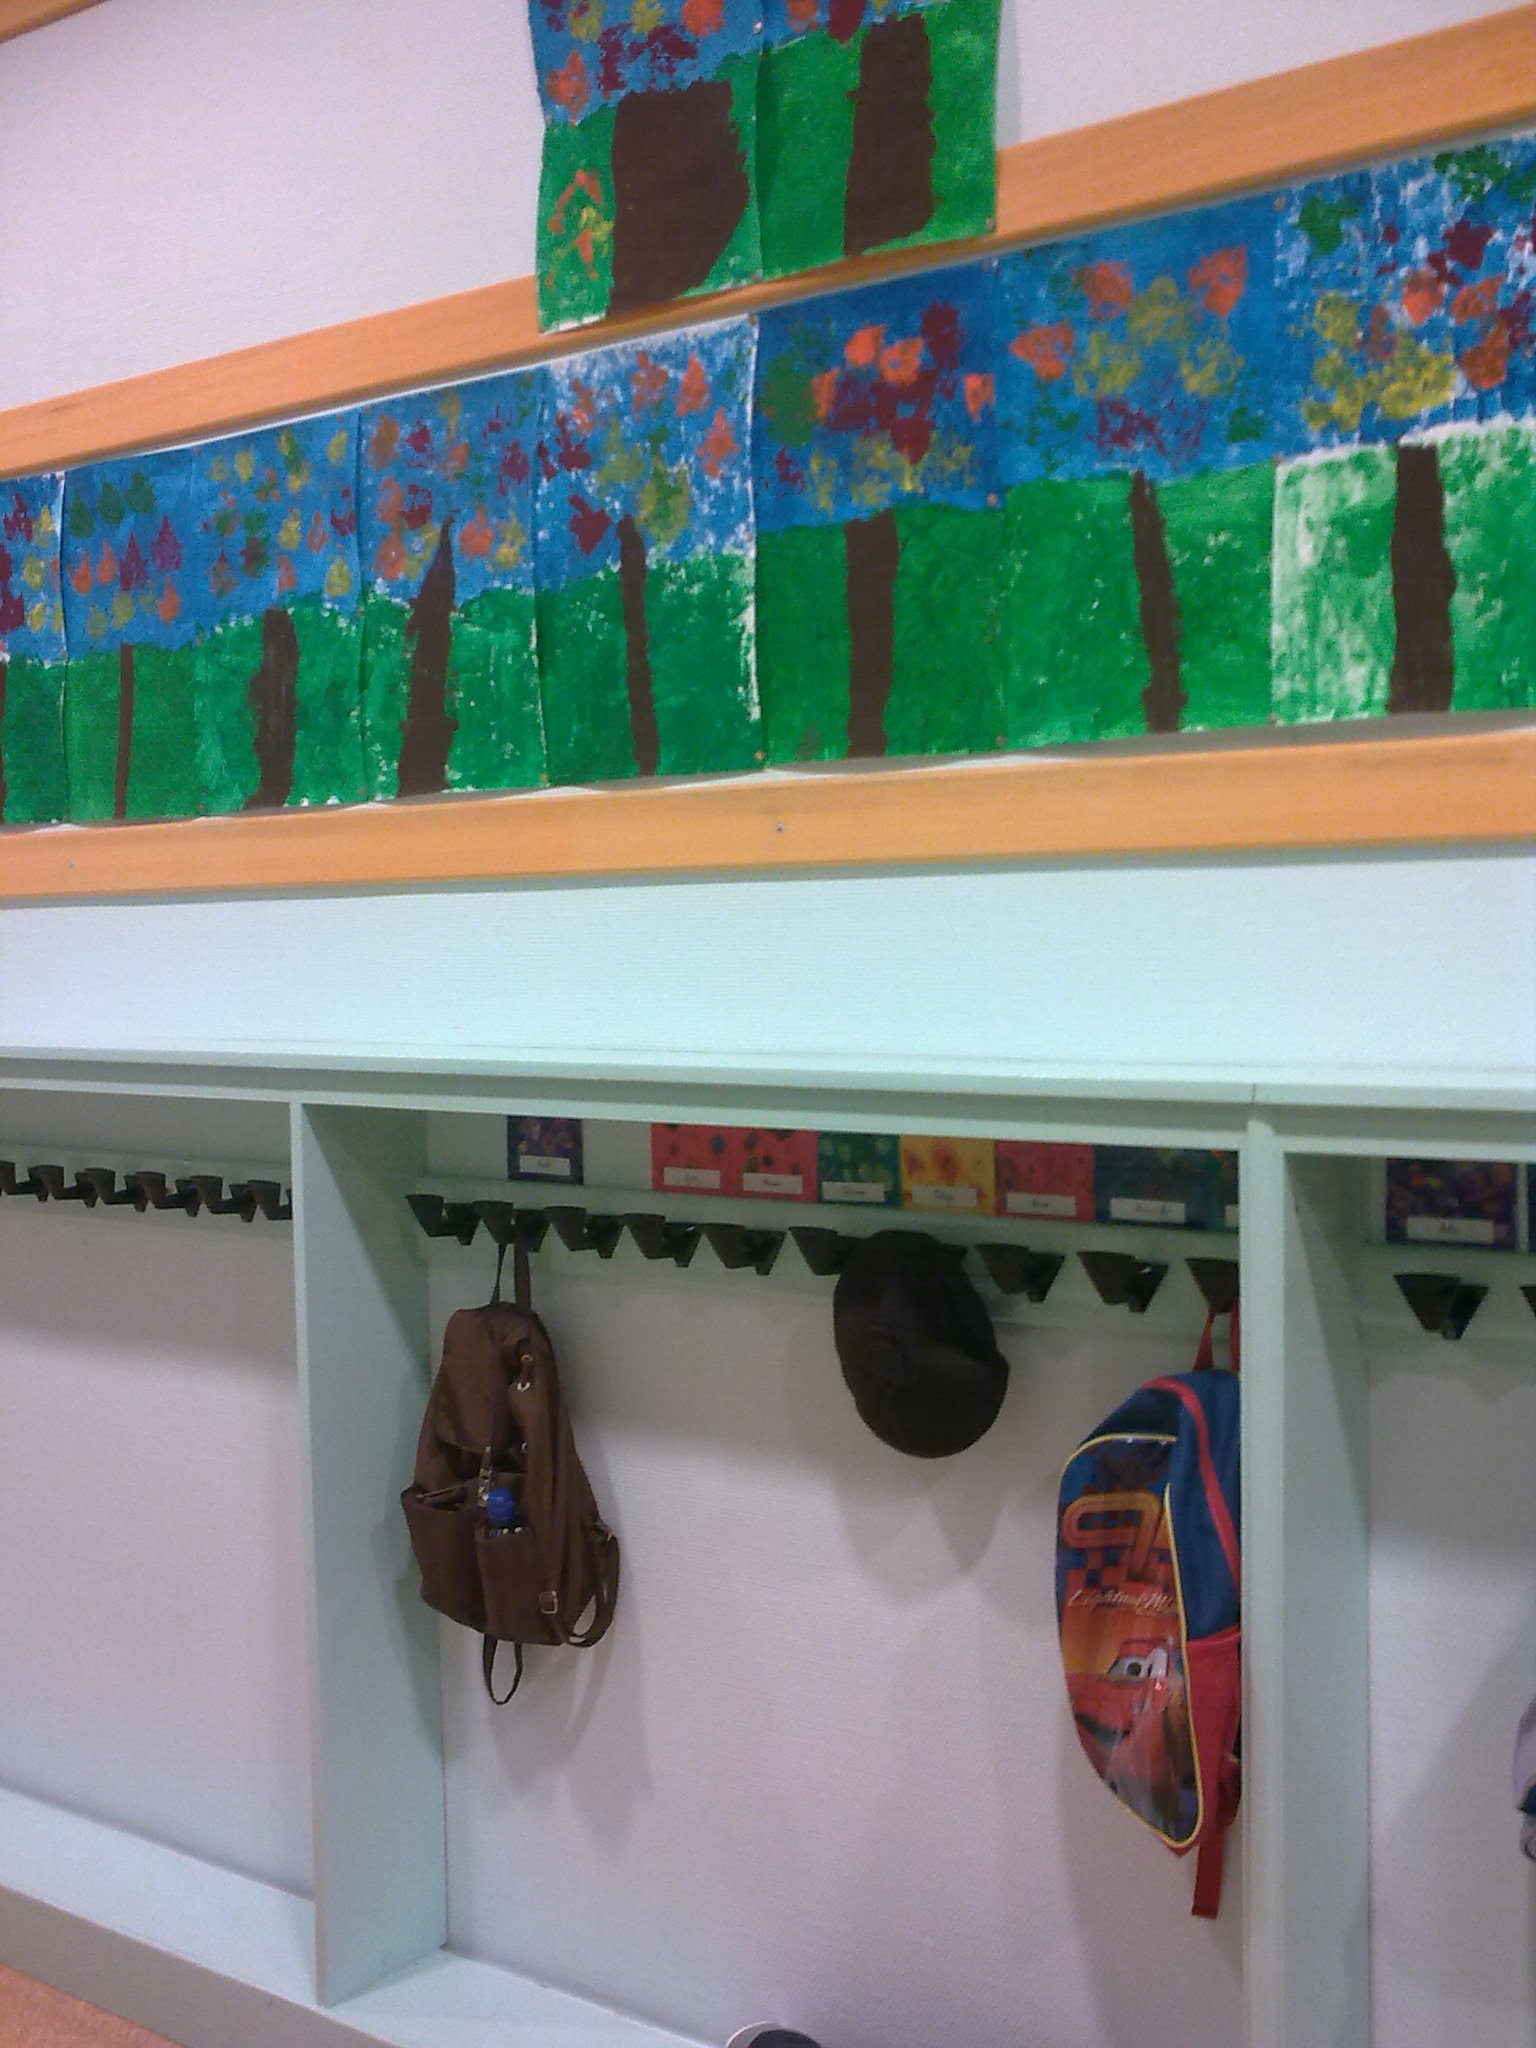
\includegraphics[height = 0.35\textheight]{./fotky/Obr9.jpg}
		\caption{
			Háčky na oblečení, polička na menší věci/šatna (viz.~\ref{prichod}).
		}
		\label{Obr9}
	\end{figure}



	\begin{figure}[tb]
		\centering
		Příloha 10\\
		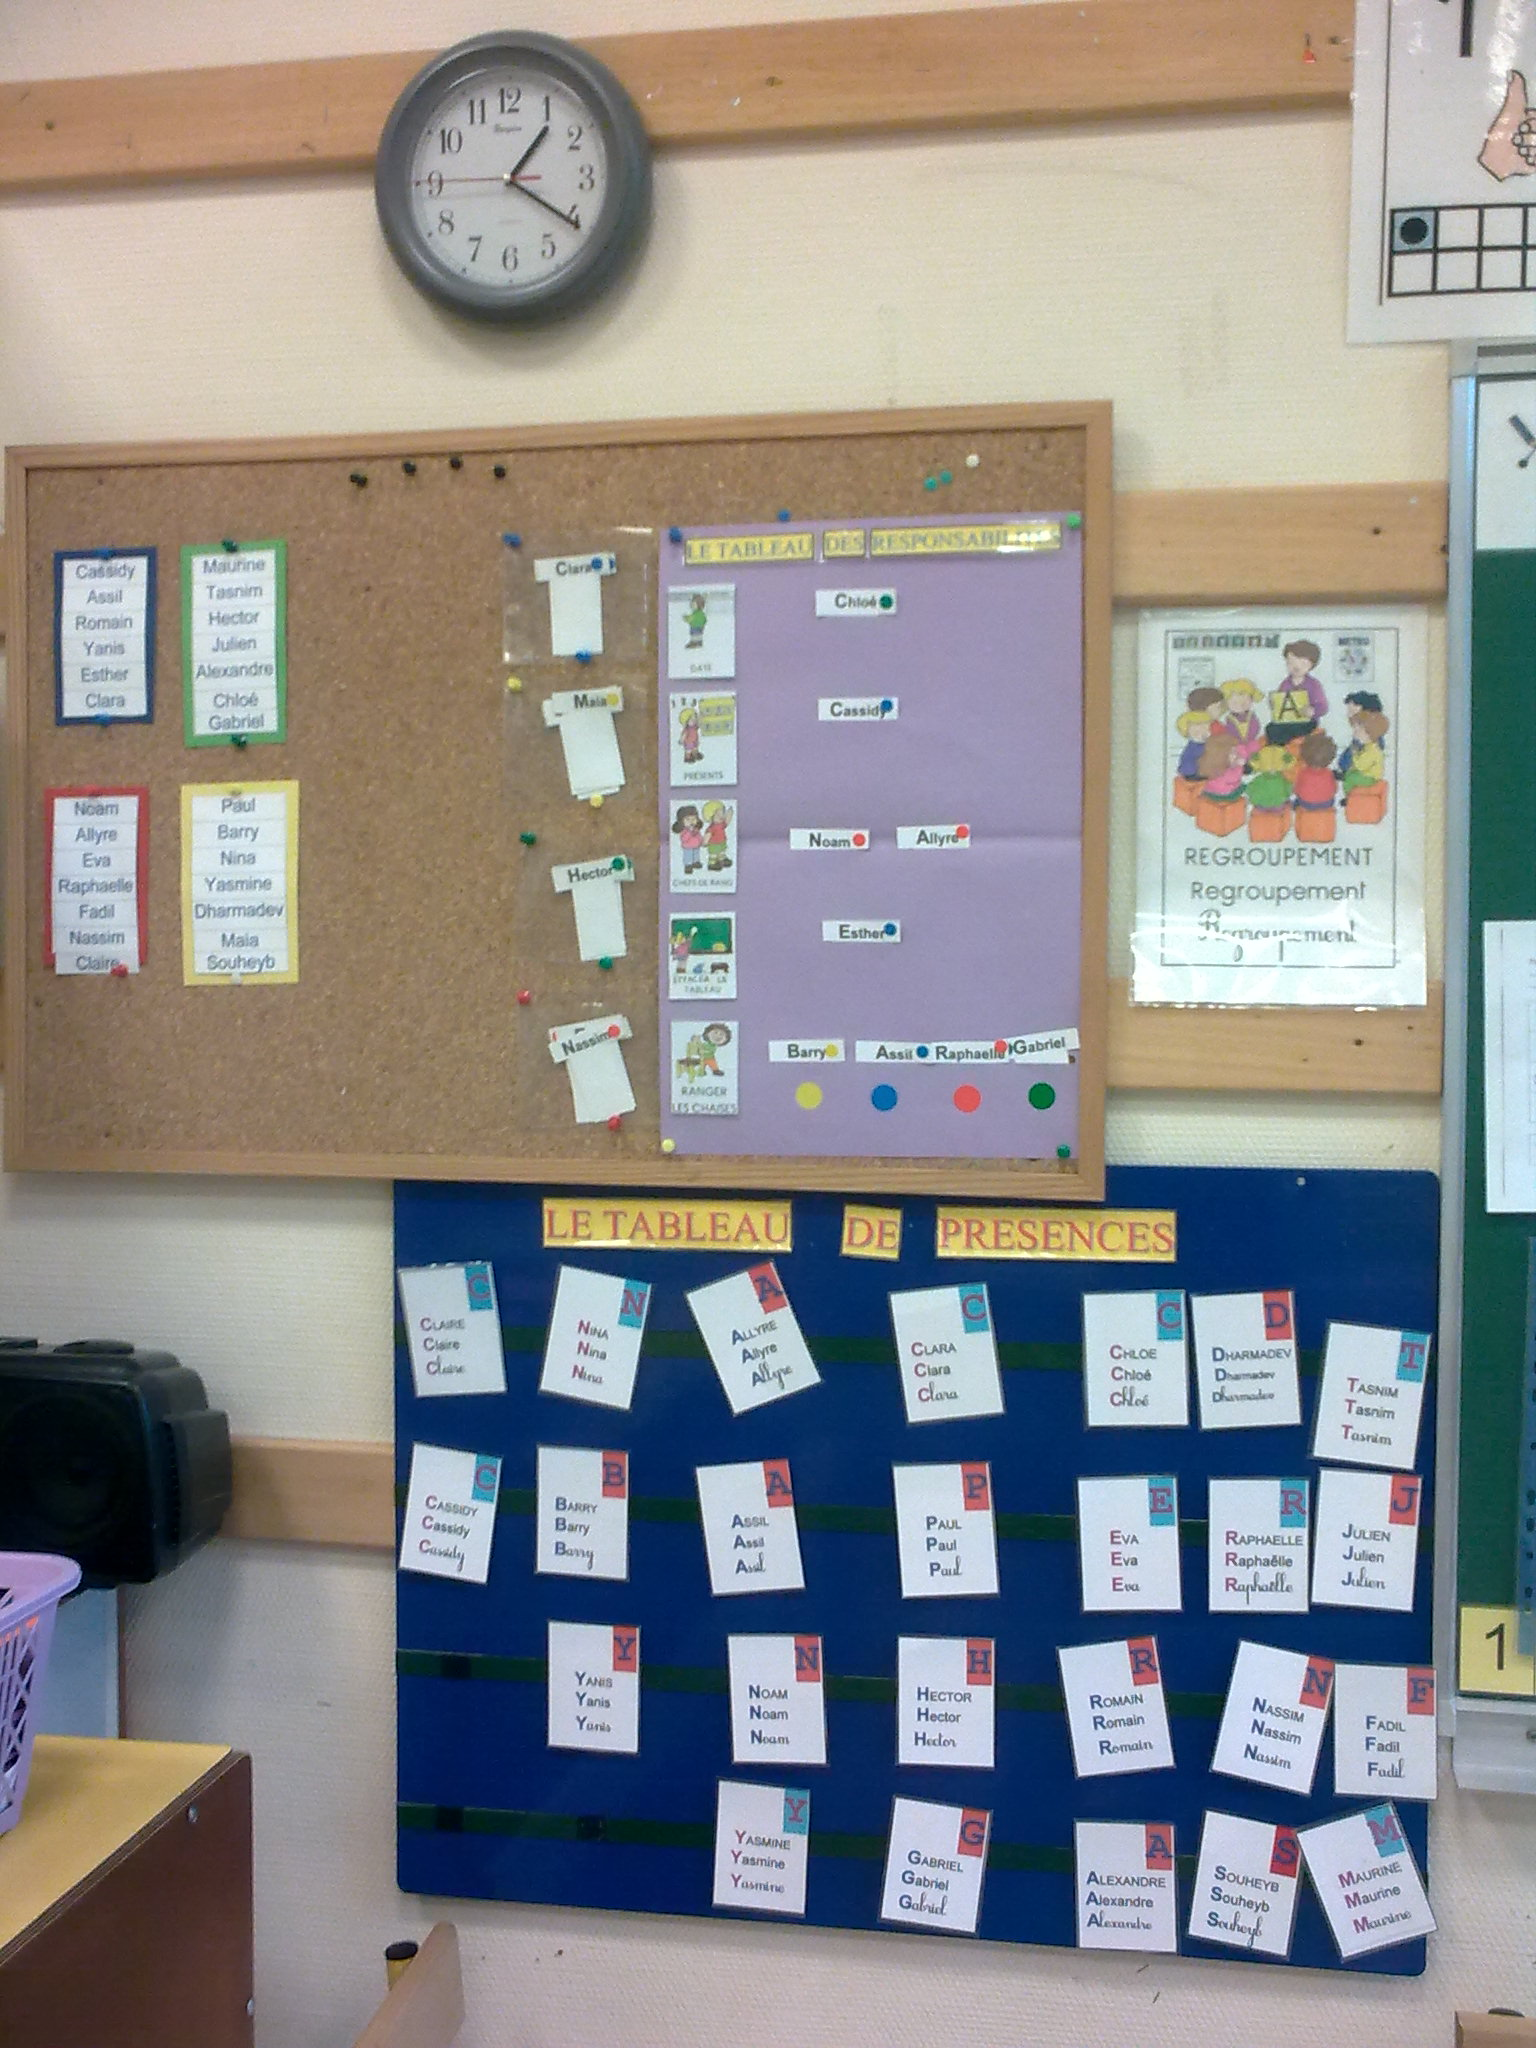
\includegraphics[height=0.35\textheight]{./fotky/Obr10.jpg}
		\caption{
			Prezence a~rozdělení do skupin na dílny (viz~\ref{prichod}).
		}
		\label{Obr10}
	\end{figure}

	\begin{figure}[tb]
		\centering
		Příloha 11\\
		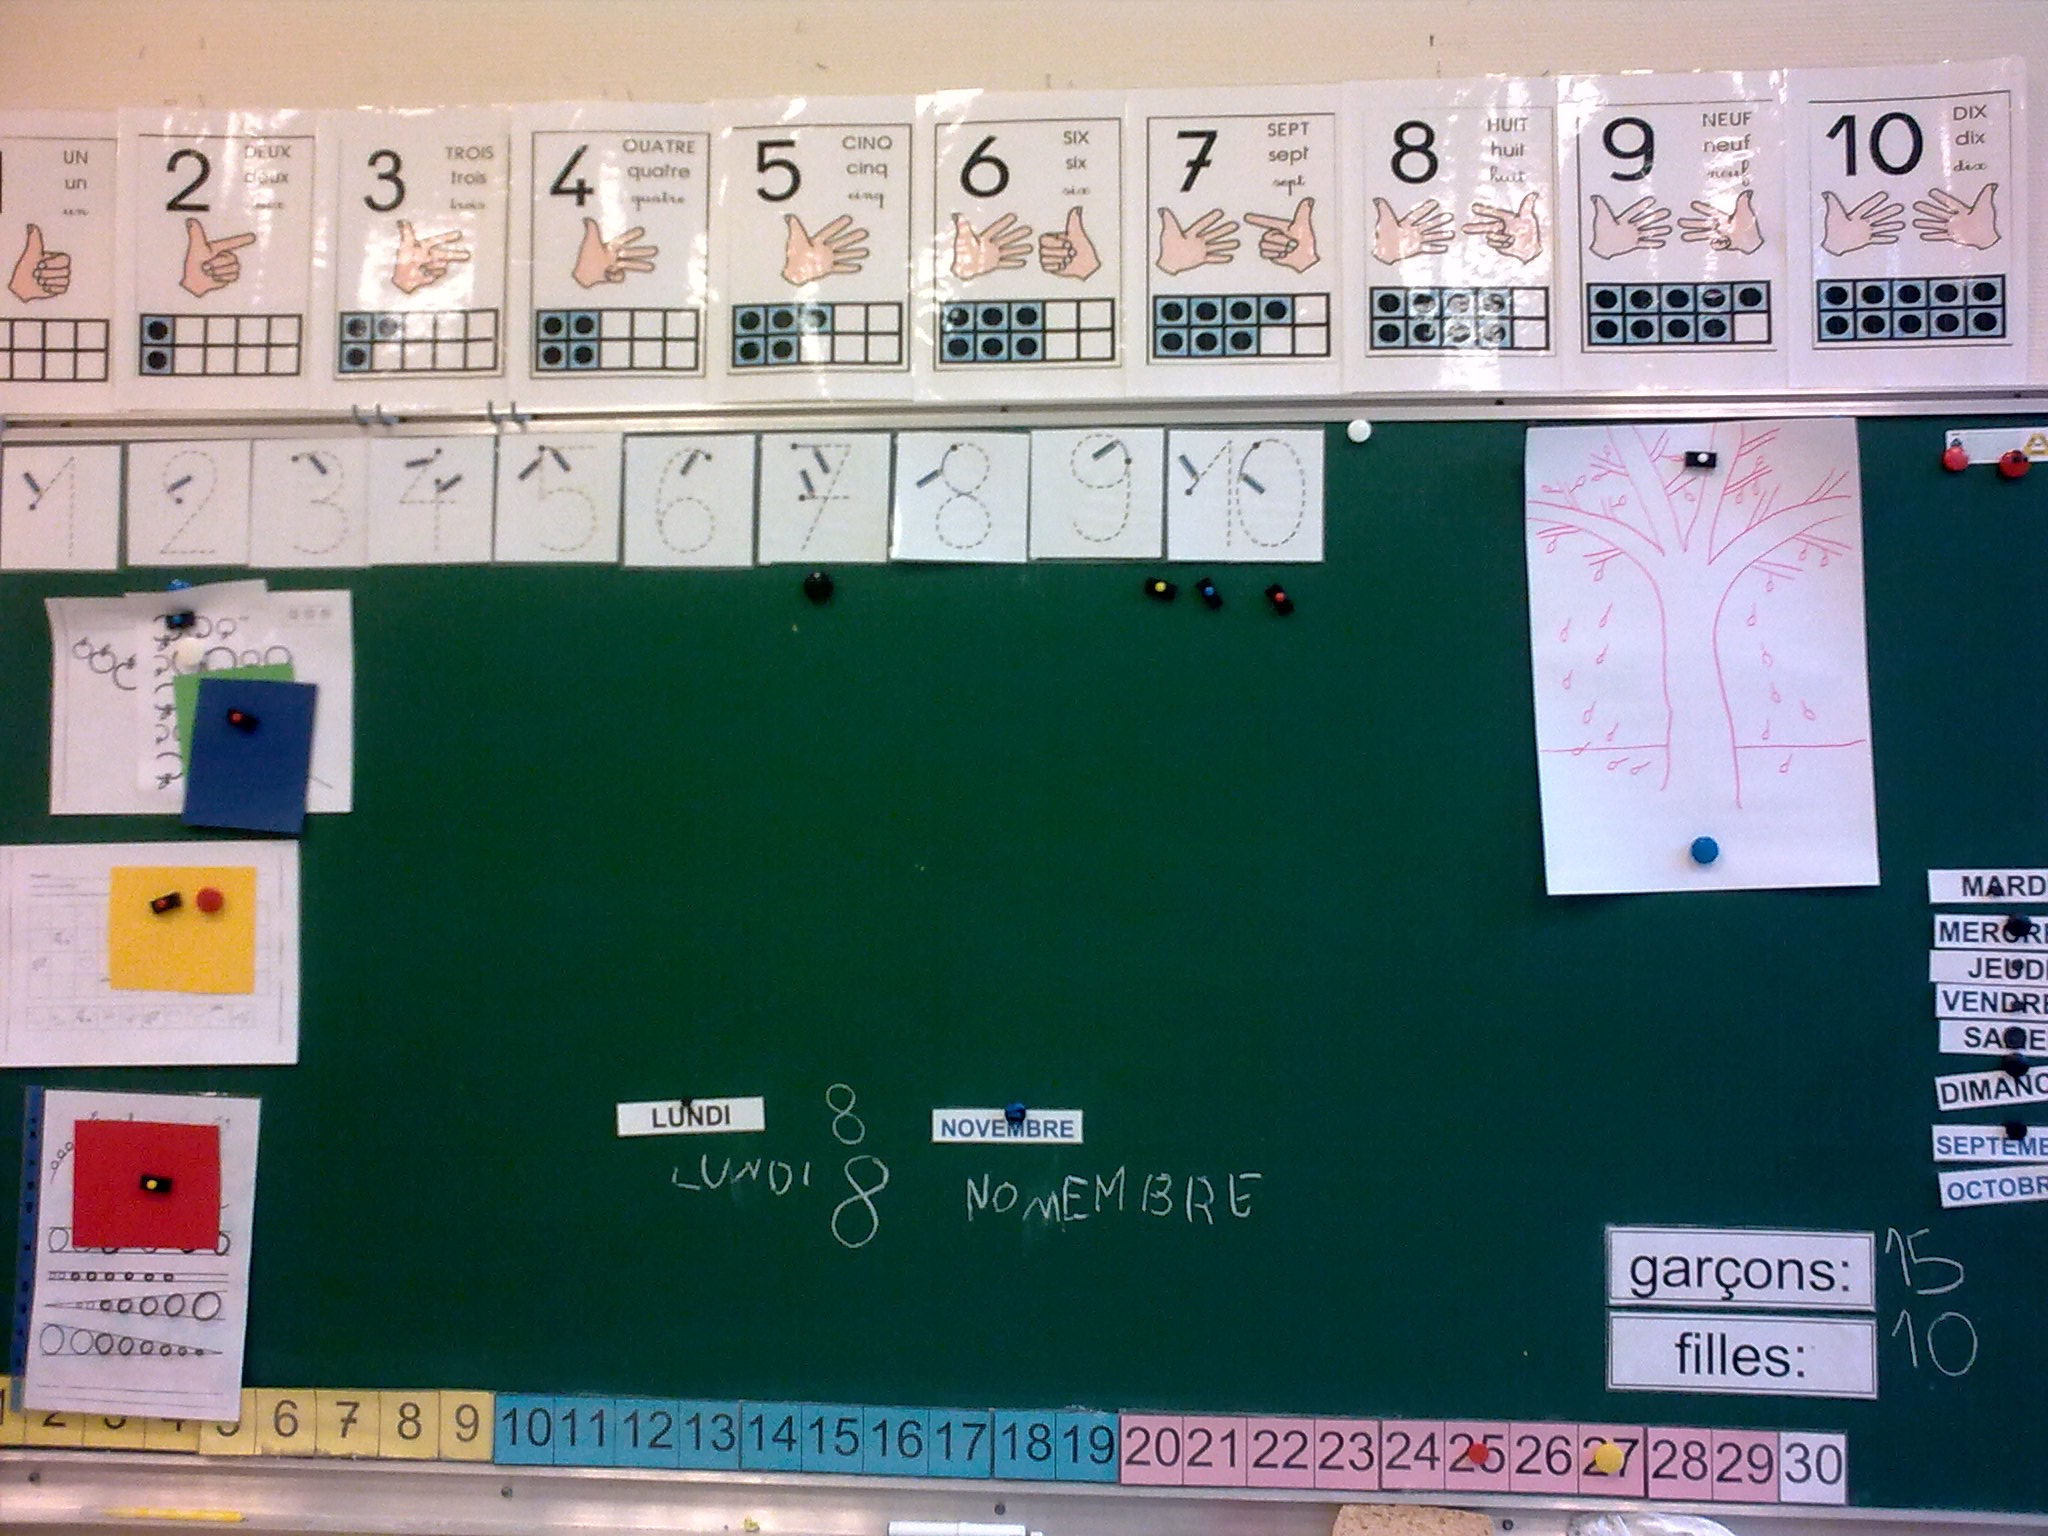
\includegraphics[height=0.35\textheight]{./fotky/Obr11.jpg}
		\caption{
			Detailní pohled na tabuli, psaní data, psaní číslic, charakteristika dílen s~týdenní nabídkou  (viz~\ref{ritualy}).
		}
		\label{Obr11}
	\end{figure}

	\begin{figure}[tb]
		\centering
		Příloha 12\\
		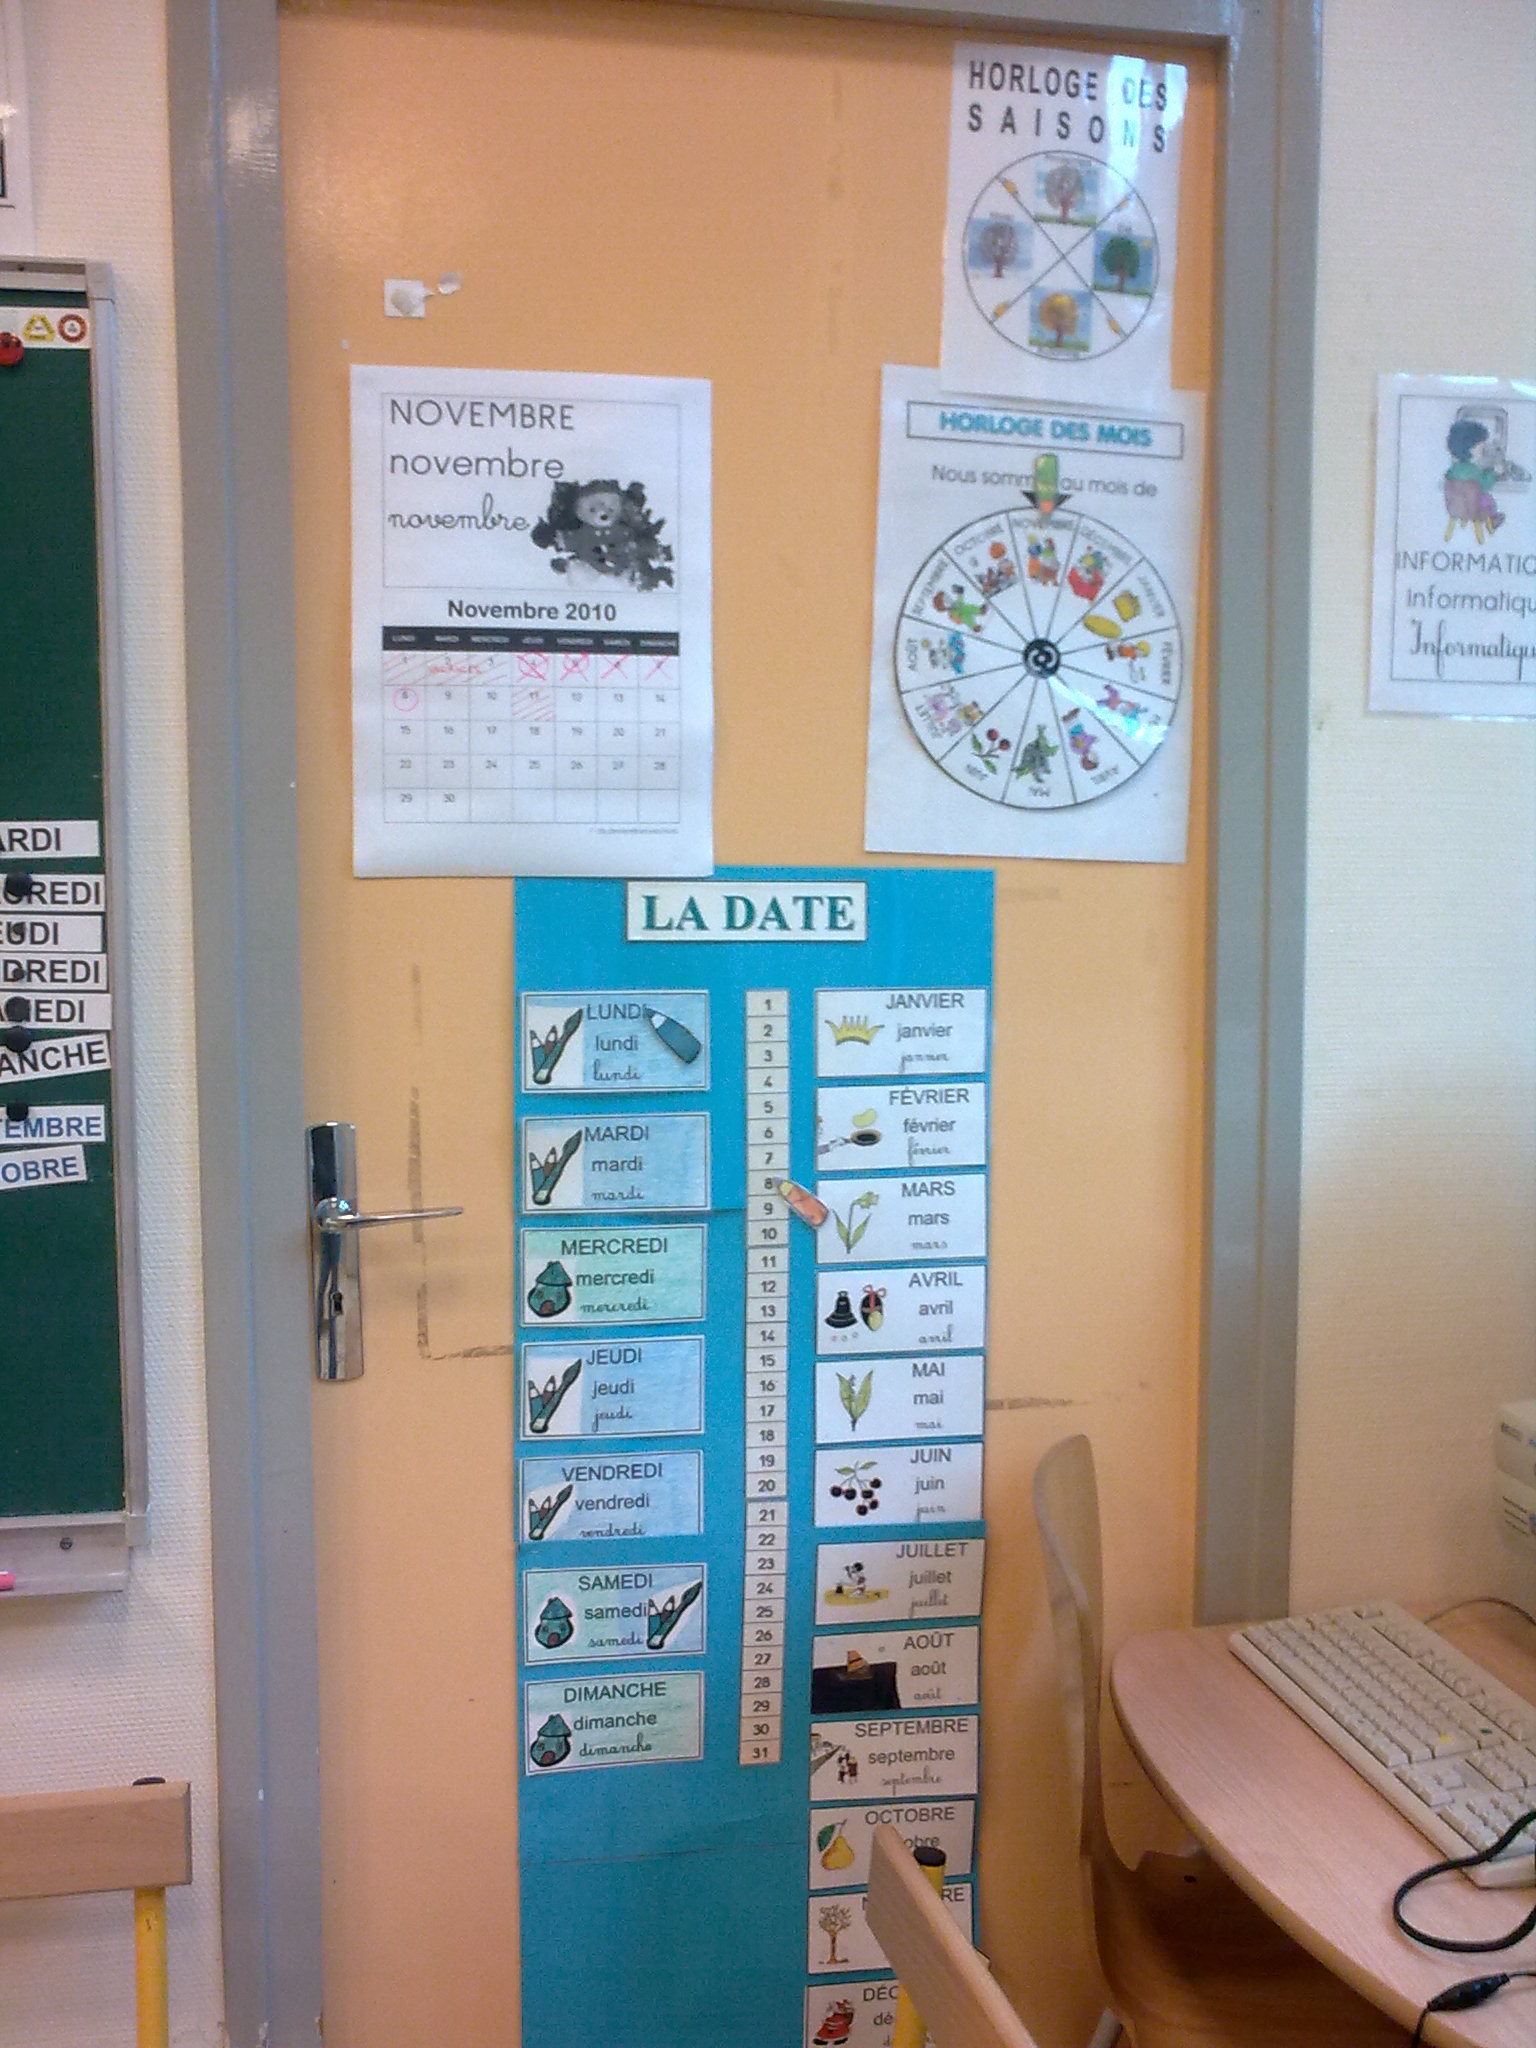
\includegraphics[height=0.35\textheight]{./fotky/Obr12.jpg}
		\caption{
			Kalendář, měsíce v~roce a~roční období (viz~\ref{ritualy}).
		}
		\label{Obr12}
	\end{figure}

	\begin{figure}[tb]
		\centering
		Příloha 13\\
		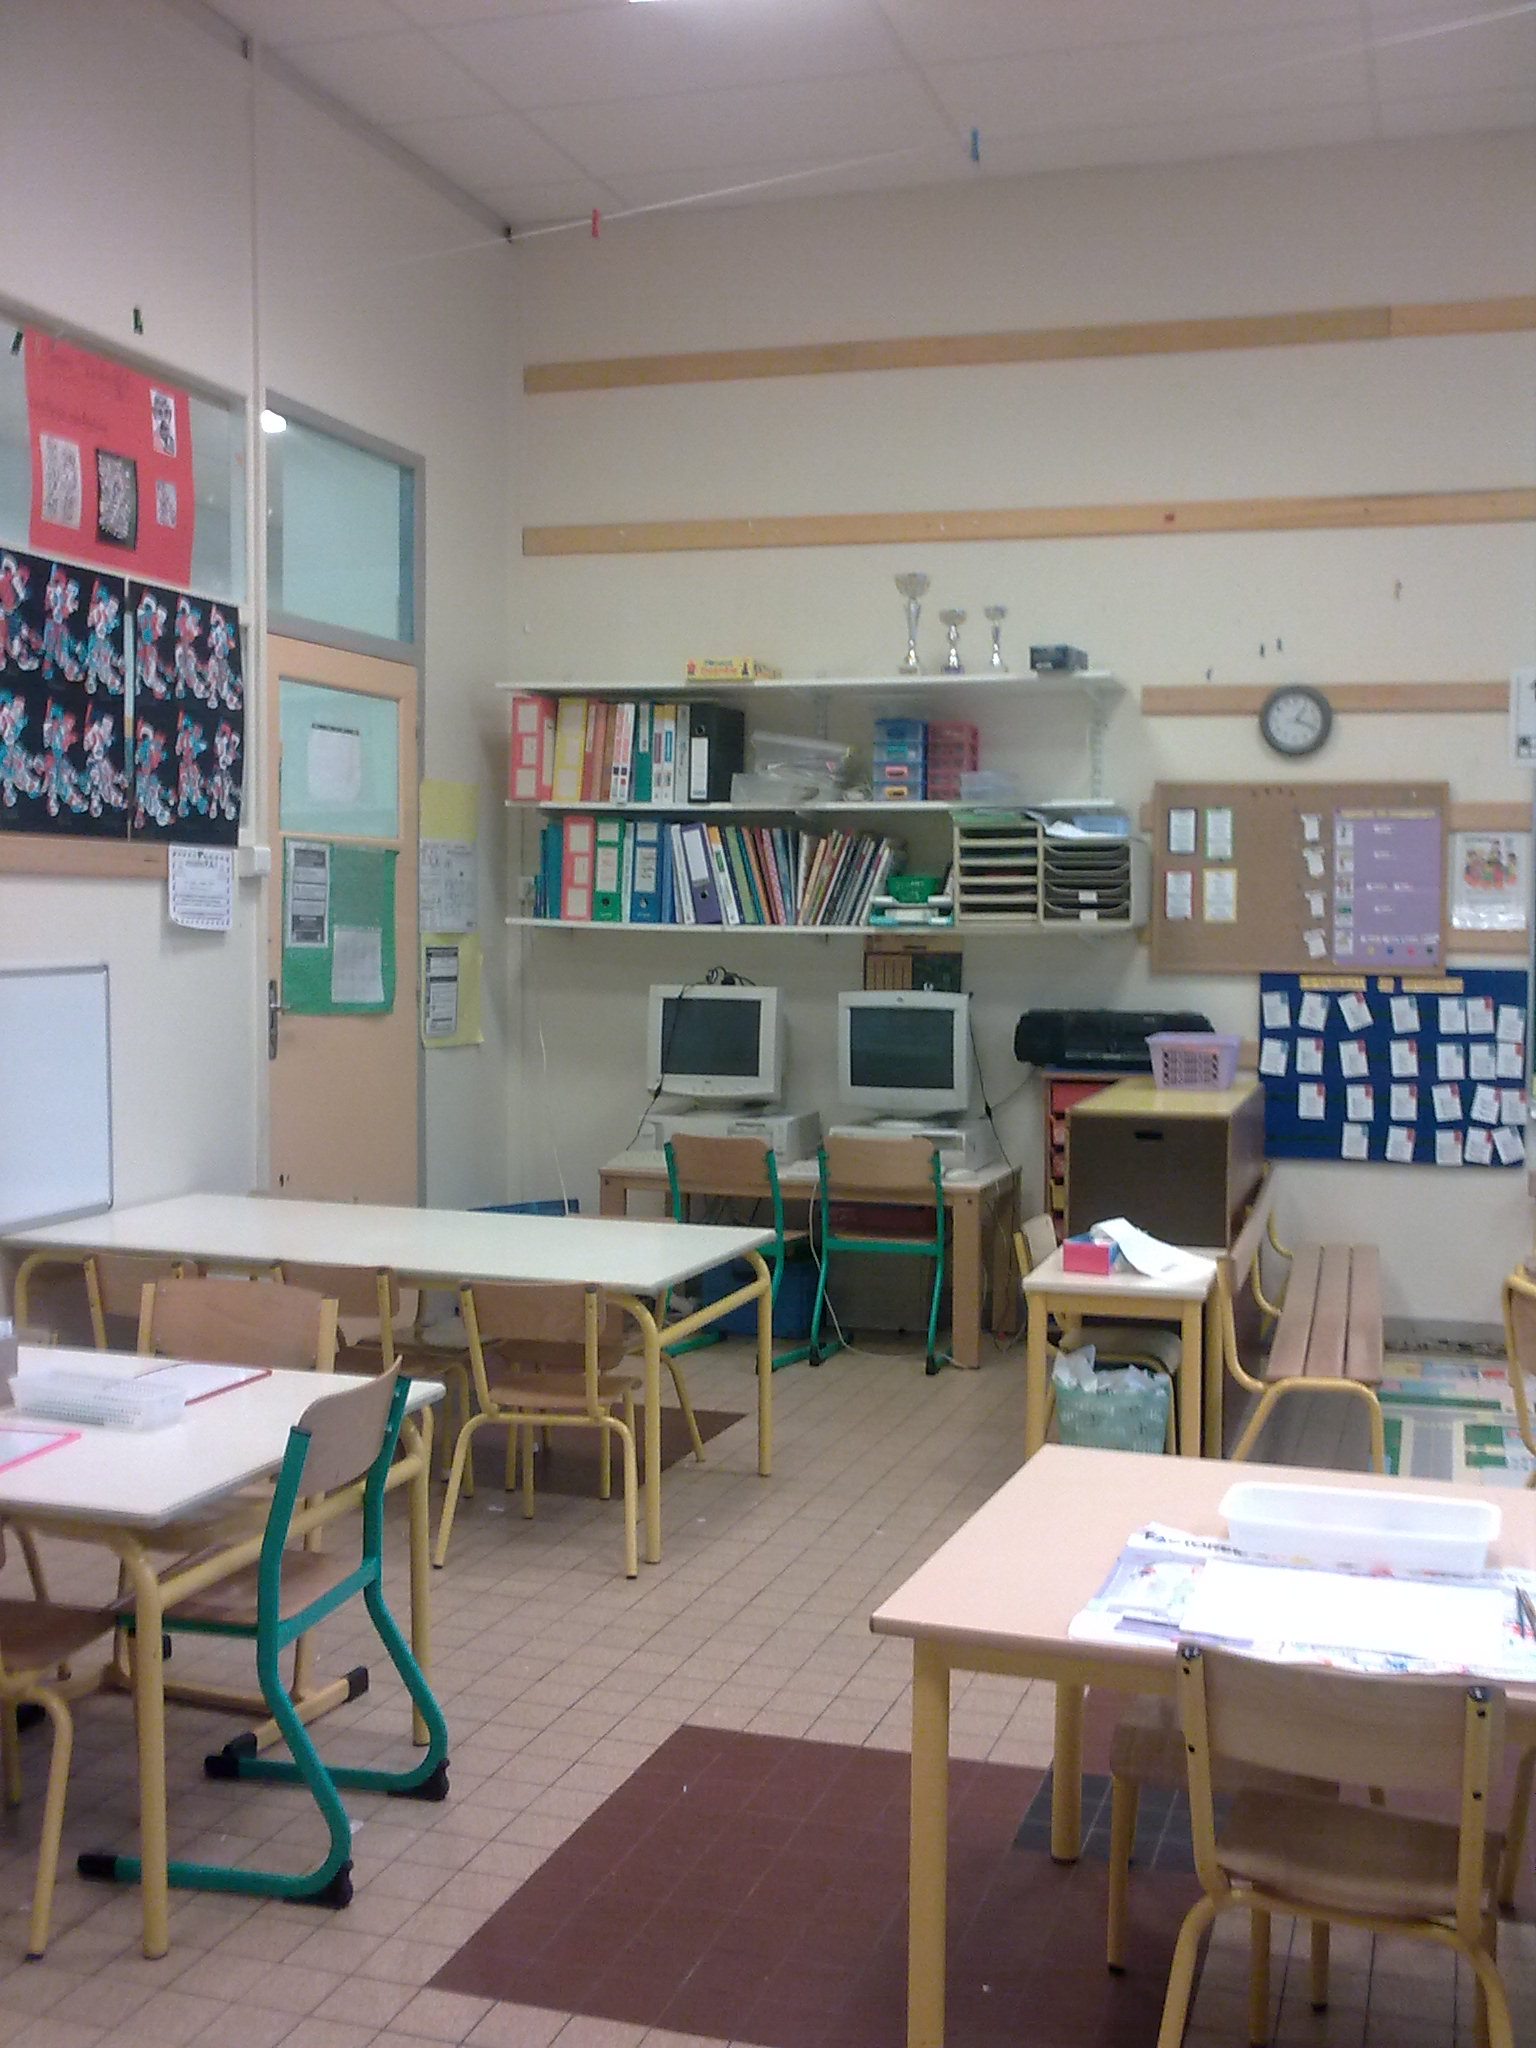
\includegraphics[height=0.35\textheight]{./fotky/Obr13.jpg}
		\caption{
			Stoly na práci při dílnách (viz~\ref{dilny}).
		}
		\label{Obr13}
	\end{figure}
	\begin{figure}[tb]
		\centering
		Příloha 14\\
		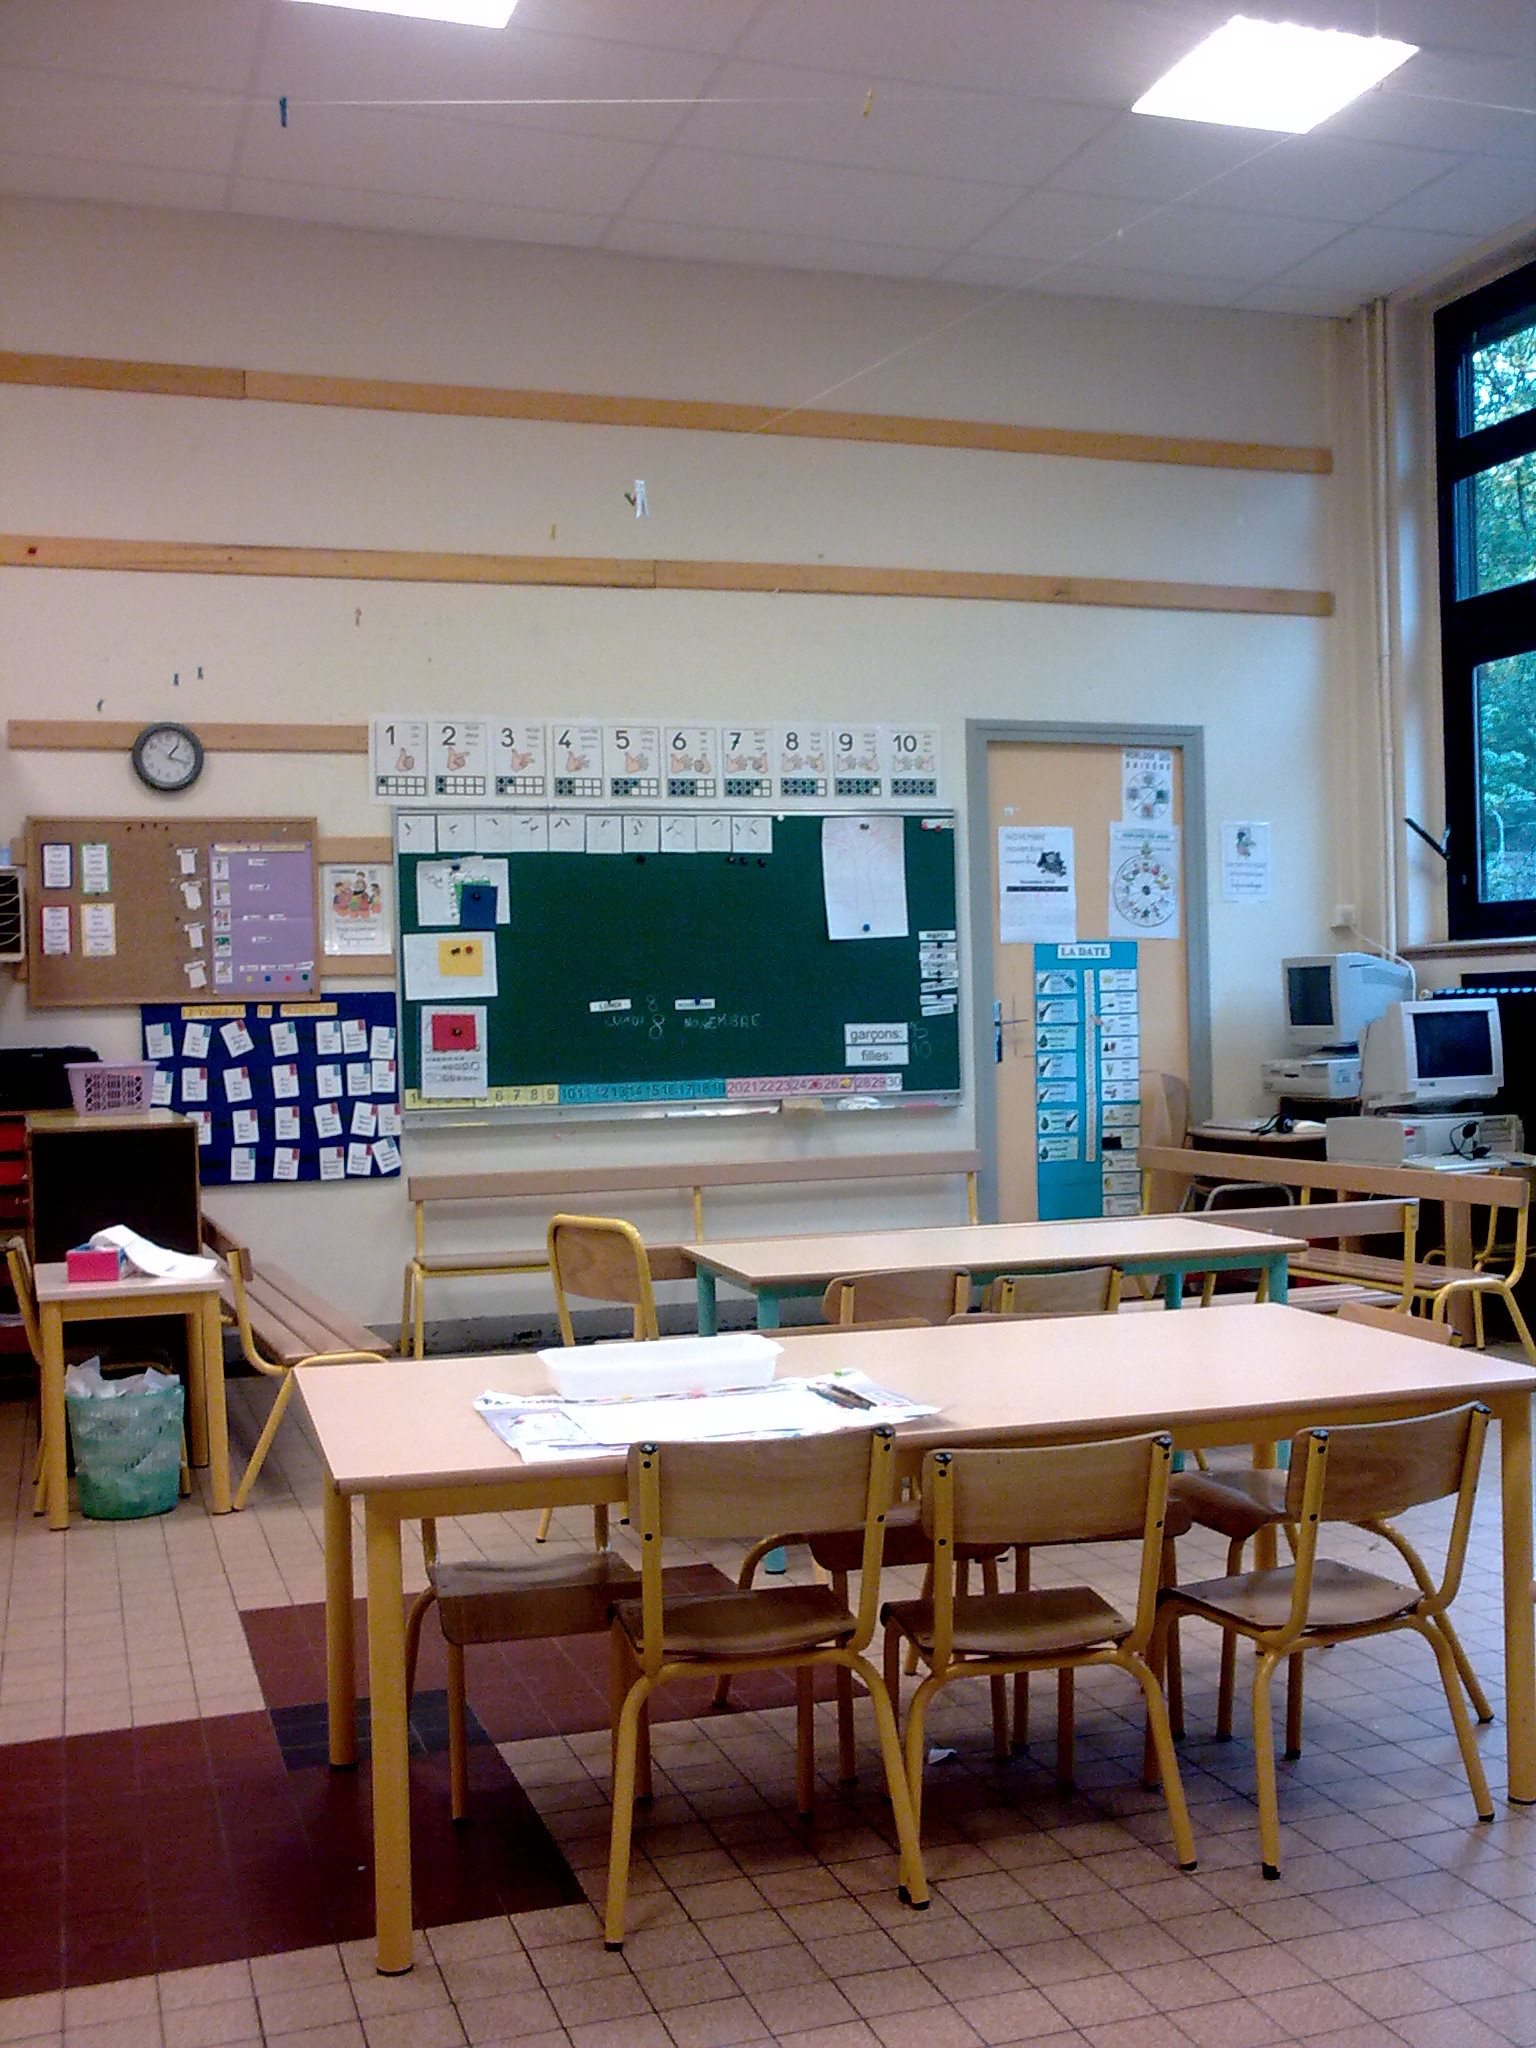
\includegraphics[height=0.35\textheight]{./fotky/Obr14.jpg}
		\caption{
			Pohled na třídu (viz~\ref{dilny}).
		}
		\label{Obr14}
	\end{figure}

	\begin{figure}[tb]
		\centering
		Příloha 15\\
		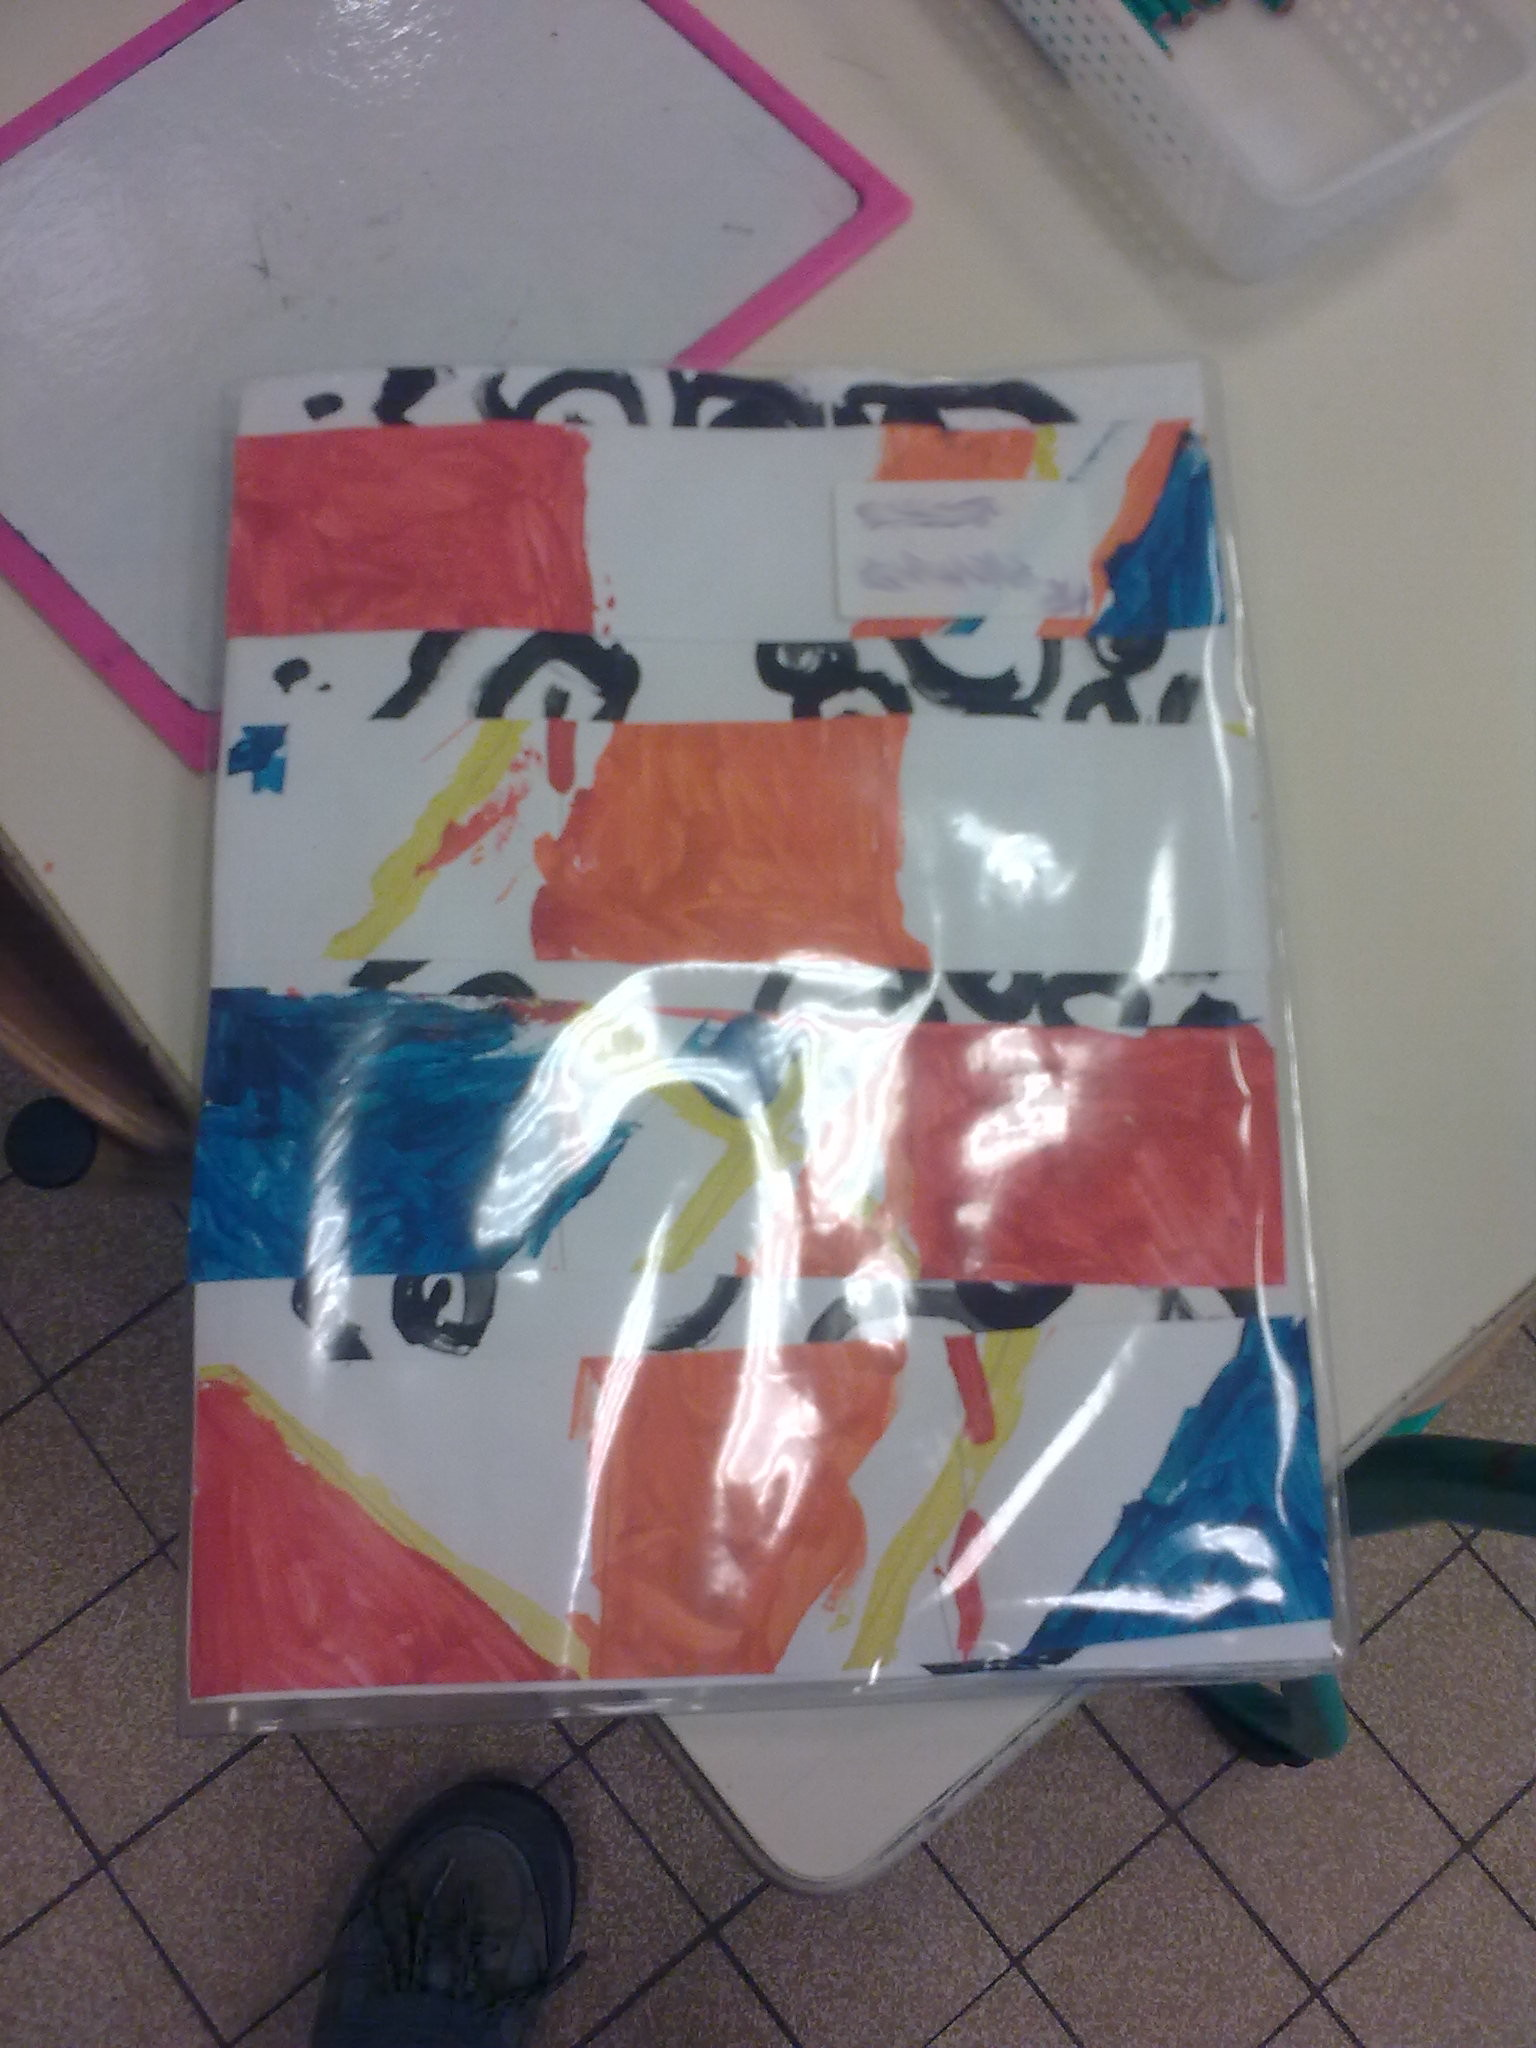
\includegraphics[height=0.35\textheight]{./fotky/Obr15.jpg}
		\caption{
			Sešit, kam si děti lepí své práce = základ portfolia (viz~\ref{dilny}).
		}
		\label{Obr15}
	\end{figure}

	\begin{figure}[tb]
		\centering
		Příloha 16\\
		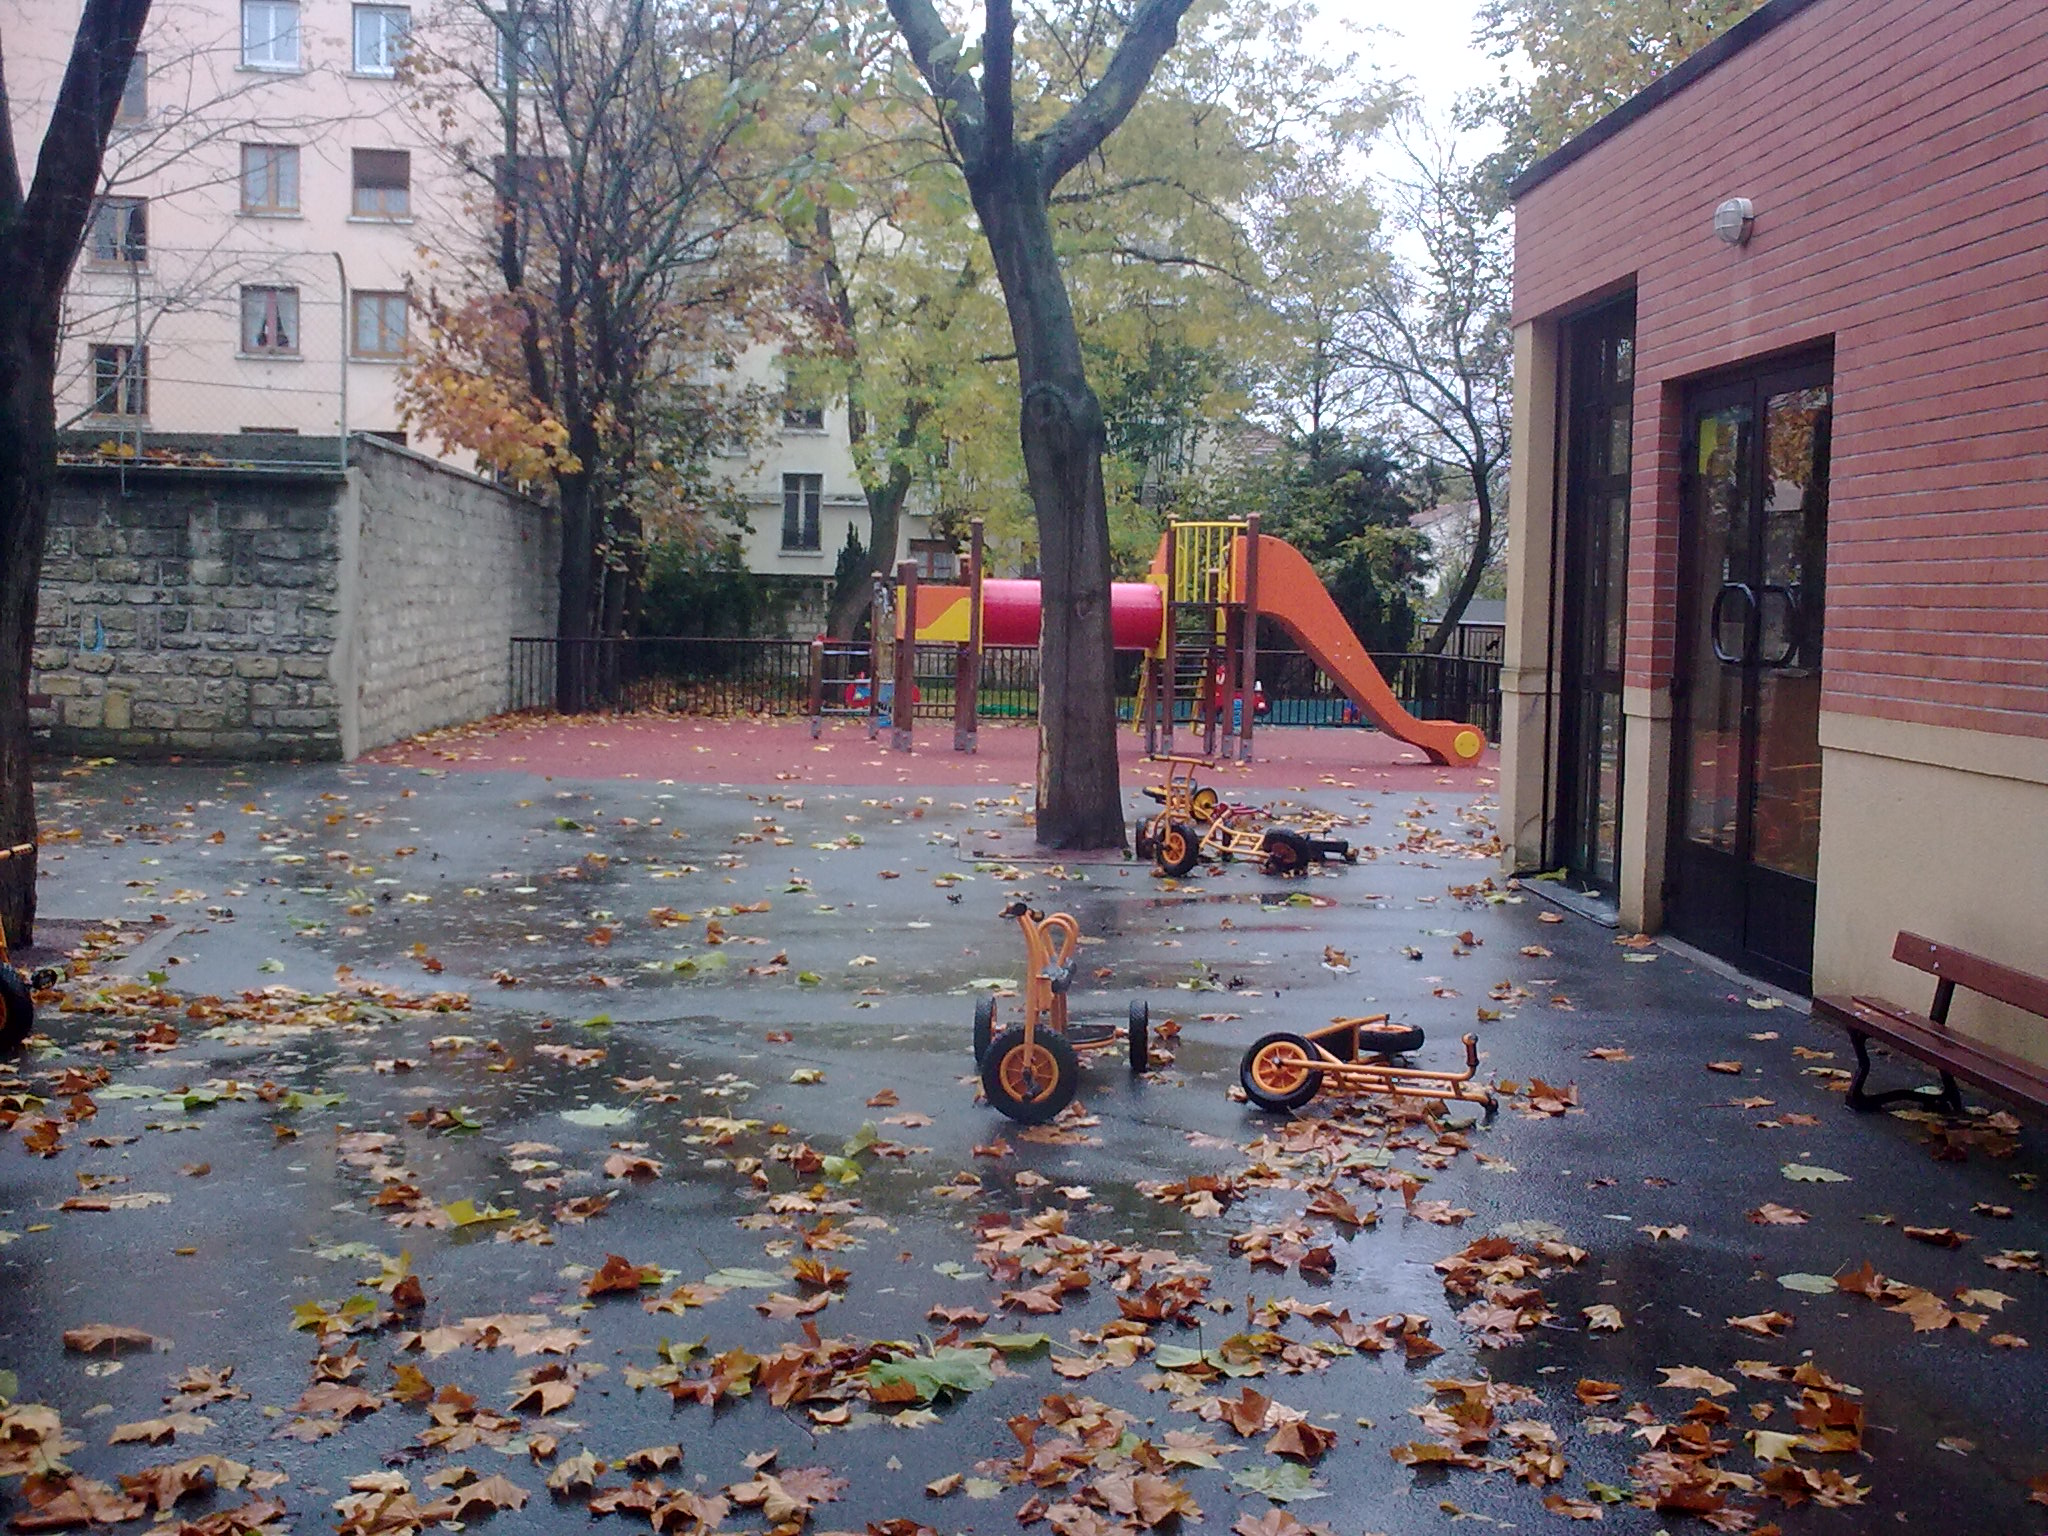
\includegraphics[height=0.35\textheight]{./fotky/Obr16.jpg}
		\caption{
			Pohled na dvůr s~prolézačkou (viz~\ref{prestavka}).
		}
		\label{Obr16}
	\end{figure}

	\begin{figure}[tb]
		\centering
		Příloha 17\\
		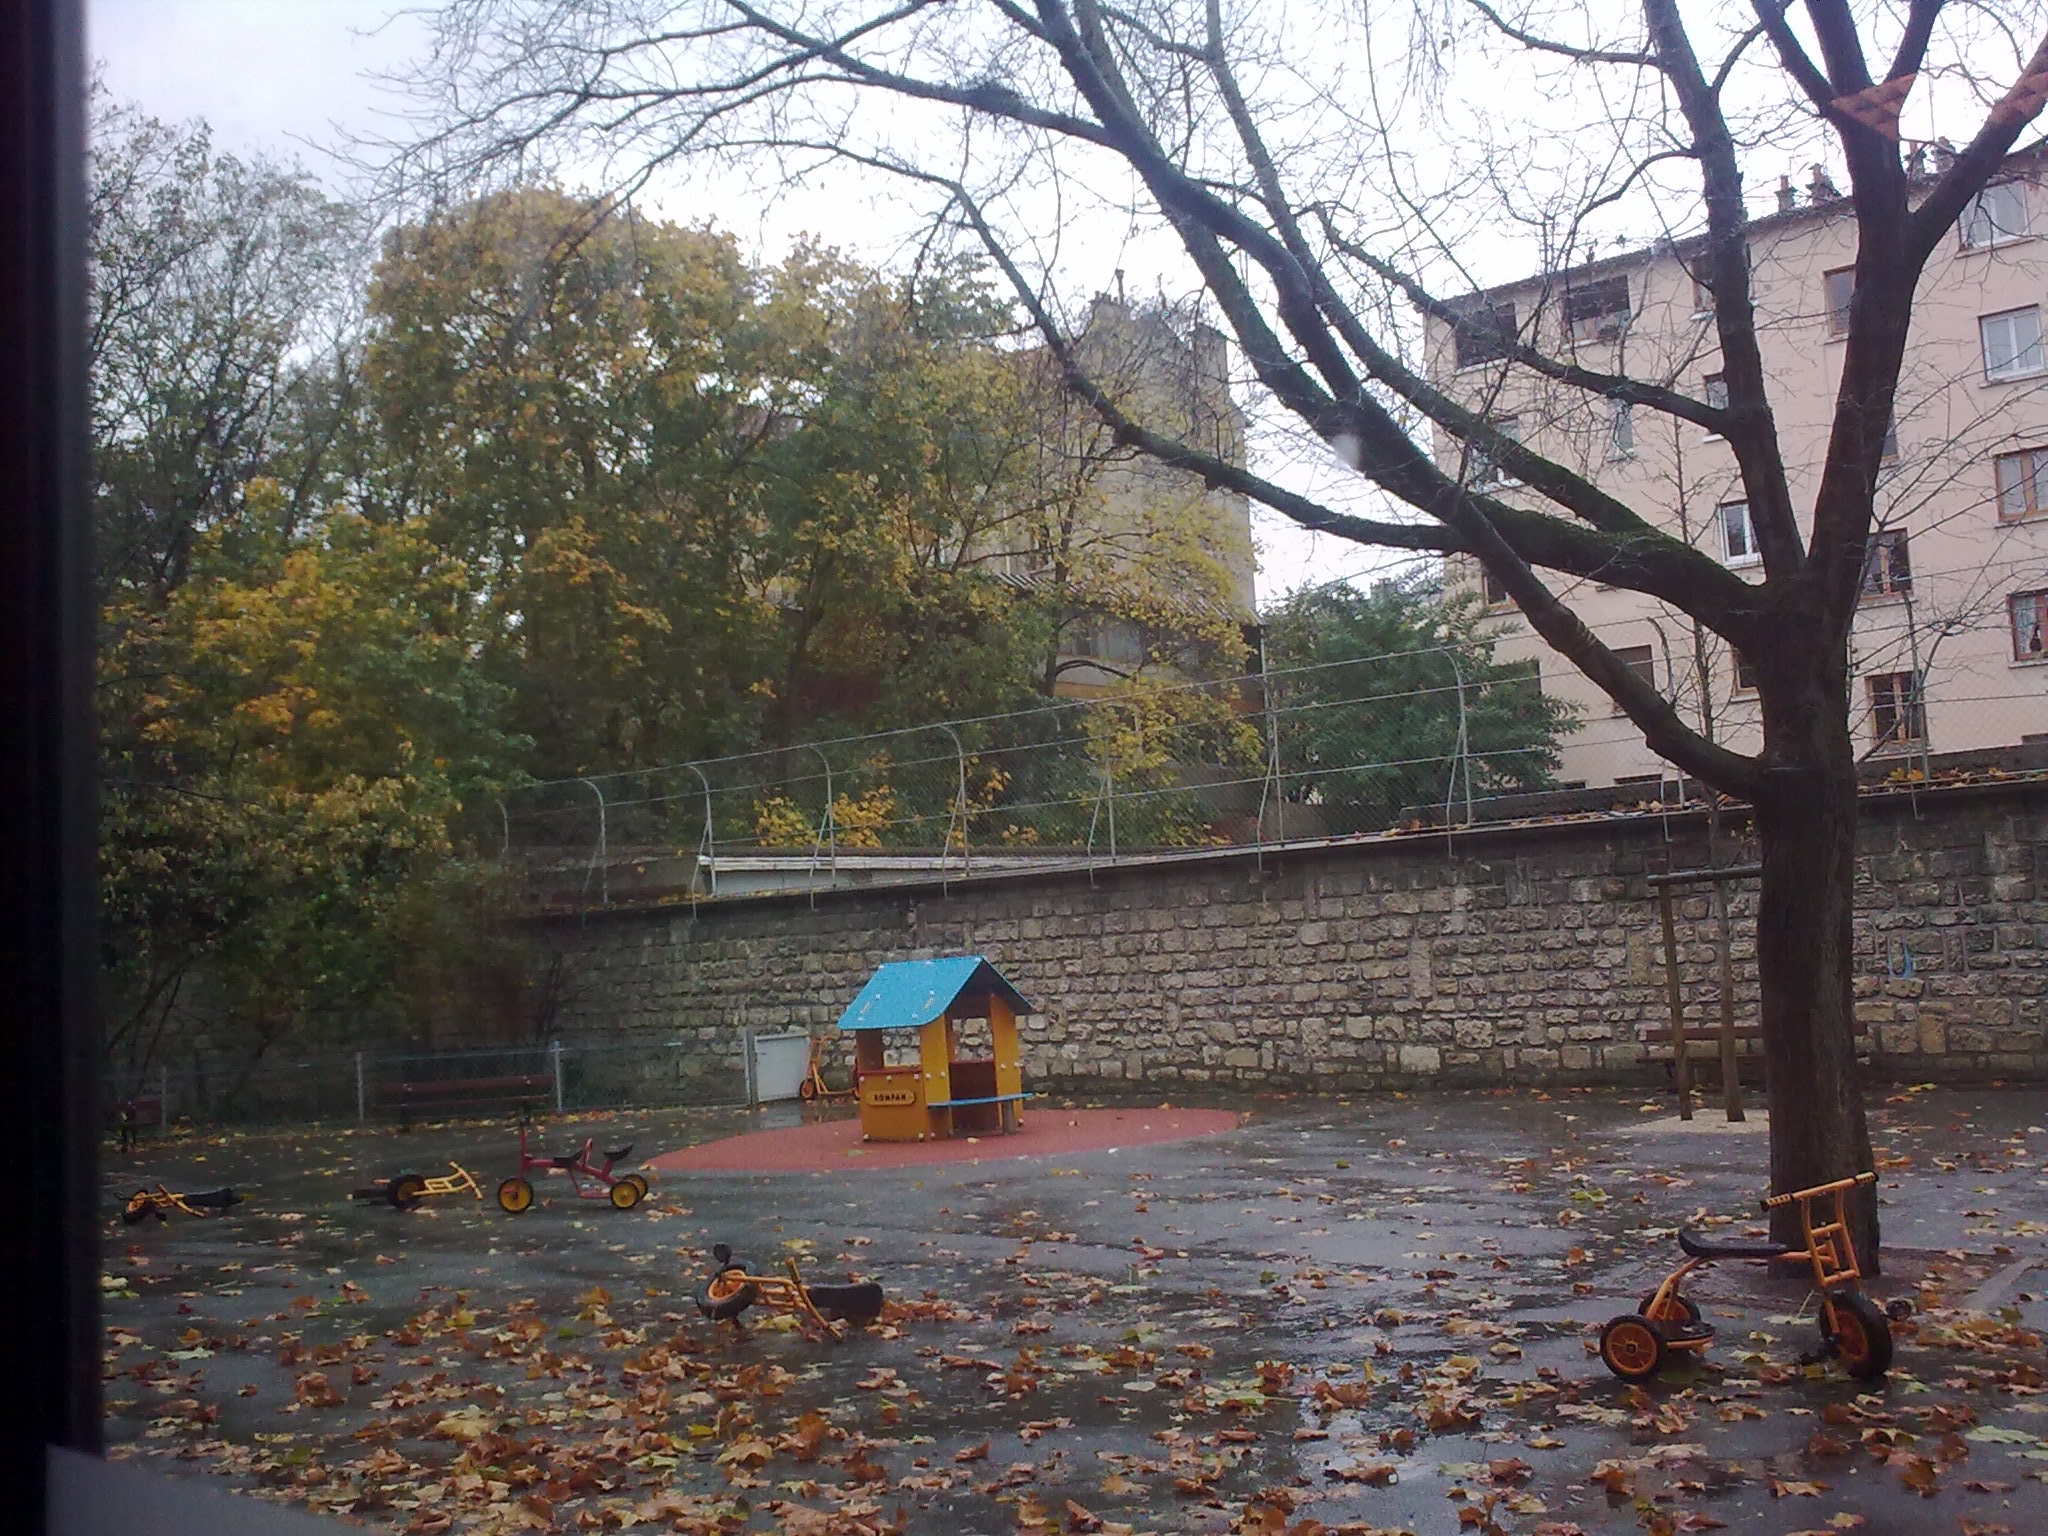
\includegraphics[height=0.35\textheight]{./fotky/Obr17.jpg}
		\caption{
			Pohled na dvůr, odstrkovadla a~domek pro děti (viz~\ref{prestavka}).
		}
		\label{Obr17}
	\end{figure}
	
	\begin{figure}[tb]
		\centering
		Příloha 19\\
		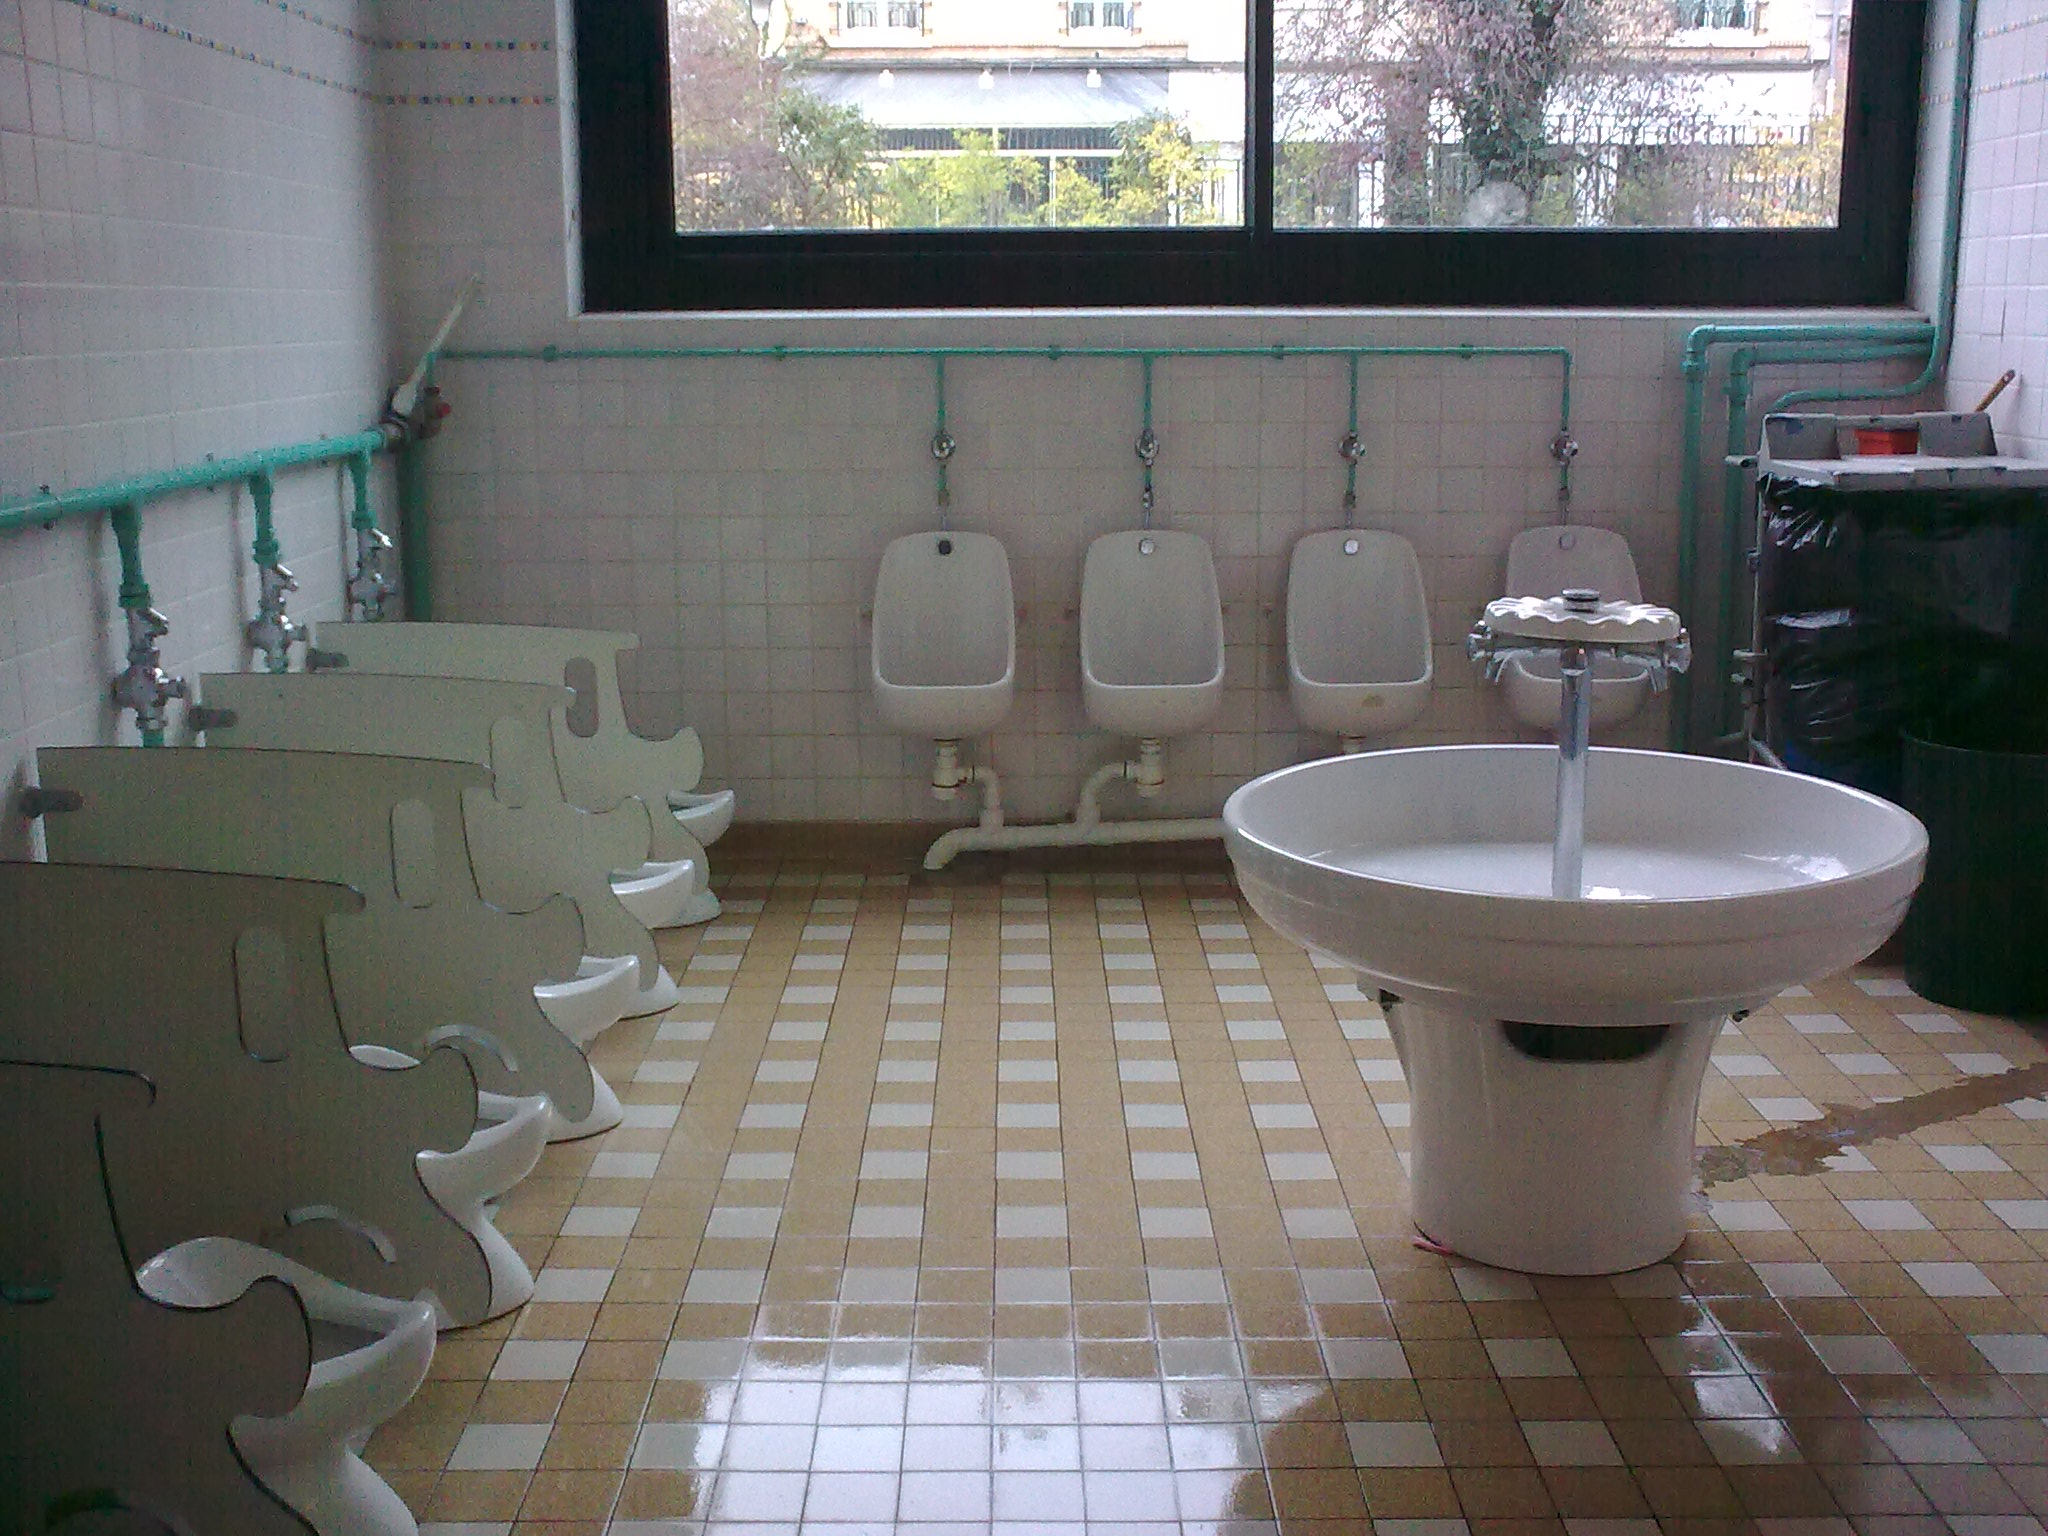
\includegraphics[height=0.35\textheight]{./fotky/Obr19.jpg}
		\caption{
			Hygienické zázemí (viz~\ref{zachody}).
		}
		\label{Obr18}
	\end{figure}


\openright
\end{document}
